\documentclass[11pt,a4paper]{article}
\usepackage[latin1]{inputenc}
\usepackage{amsmath}
\usepackage{graphicx}
\usepackage{listings}
\usepackage{tabularx, booktabs}
\newcolumntype{Y}{>{\centering\arraybackslash}X}
\usepackage{array}
\usepackage{amsfonts}
\usepackage{subfig}
\usepackage{amssymb}
\usepackage{hyperref}
\usepackage{float}
\usepackage{verbatim}
\usepackage{microtype}
\usepackage{cite}
\usepackage[parfill]{parskip} % REMOVE INDENTS
\usepackage{wrapfig}
\usepackage{textcomp}
\setcounter{secnumdepth}{5}
\usepackage{longtable}
\usepackage{array}
\usepackage{multirow}
\usepackage{rotating}
\usepackage{lscape}
\usepackage{chngcntr}%per section figure numbers
\usepackage{array}
\counterwithin{table}{section}
\counterwithin{figure}{section}
\usepackage[margin=1cm]{geometry}

\begin{document}

\section{Sensitivity to Position of Cement}

The variation found in the experimentally augmented, scanned, segmented and modelled specimens, regardless of cement volume fill prompts investigation into the effect of the position of the cement.
Table XX shows the effect of moving a volumes of cement that equals approximately four \% of the total vertebral volume between the anterior, posterior, center, superior and inferior regions of the vertebrl body.
Moving the cement volume to the anterior and centre of the vertebral body makes small differences to the stiffness, while moving the volume to the posterior portion of the vertebral body greatly increased the stiffness.
Similarly moving the volume to the superior and inferior portions of the vertebral body also increase the stiffness significantly.

\begin{landscape}
\begin{longtable}{|m{11cm}|m{11cm}|m{4cm}|}
   \\ \hline
Stress & Strain & Details \\ \hline
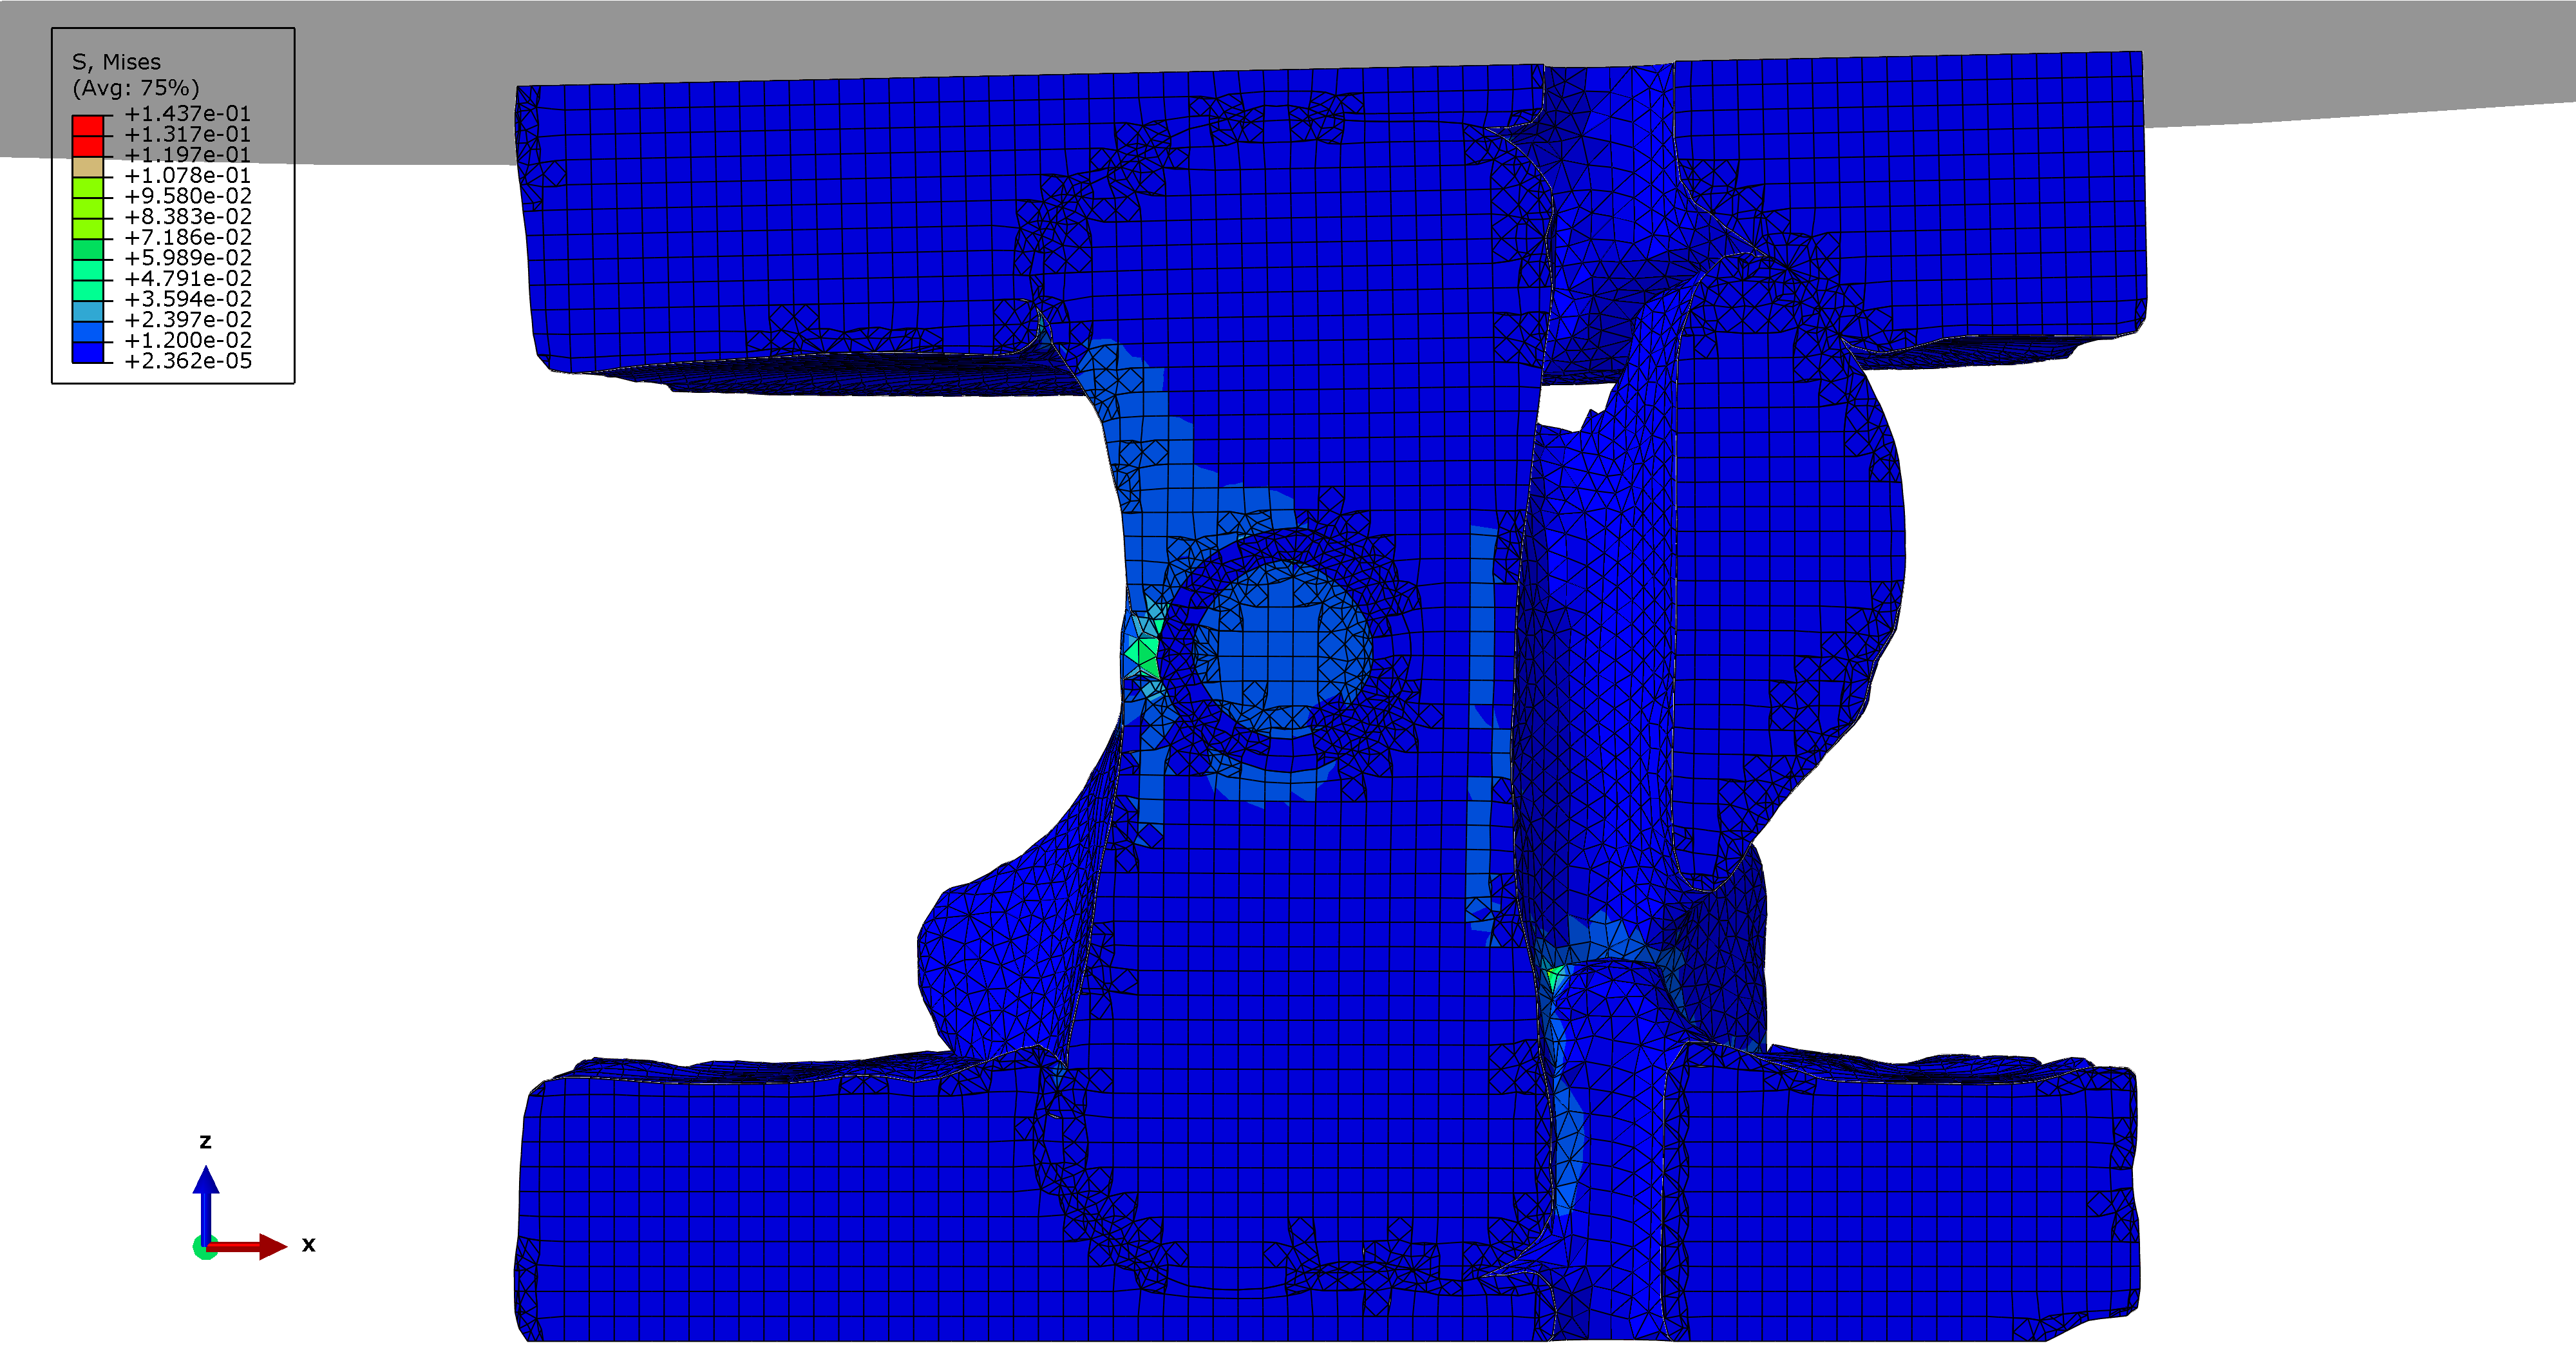
\includegraphics[width=10cm]{images/T2_CC2_intact_MM_cement_Anterior_ABAQUS_Stress.png}   & 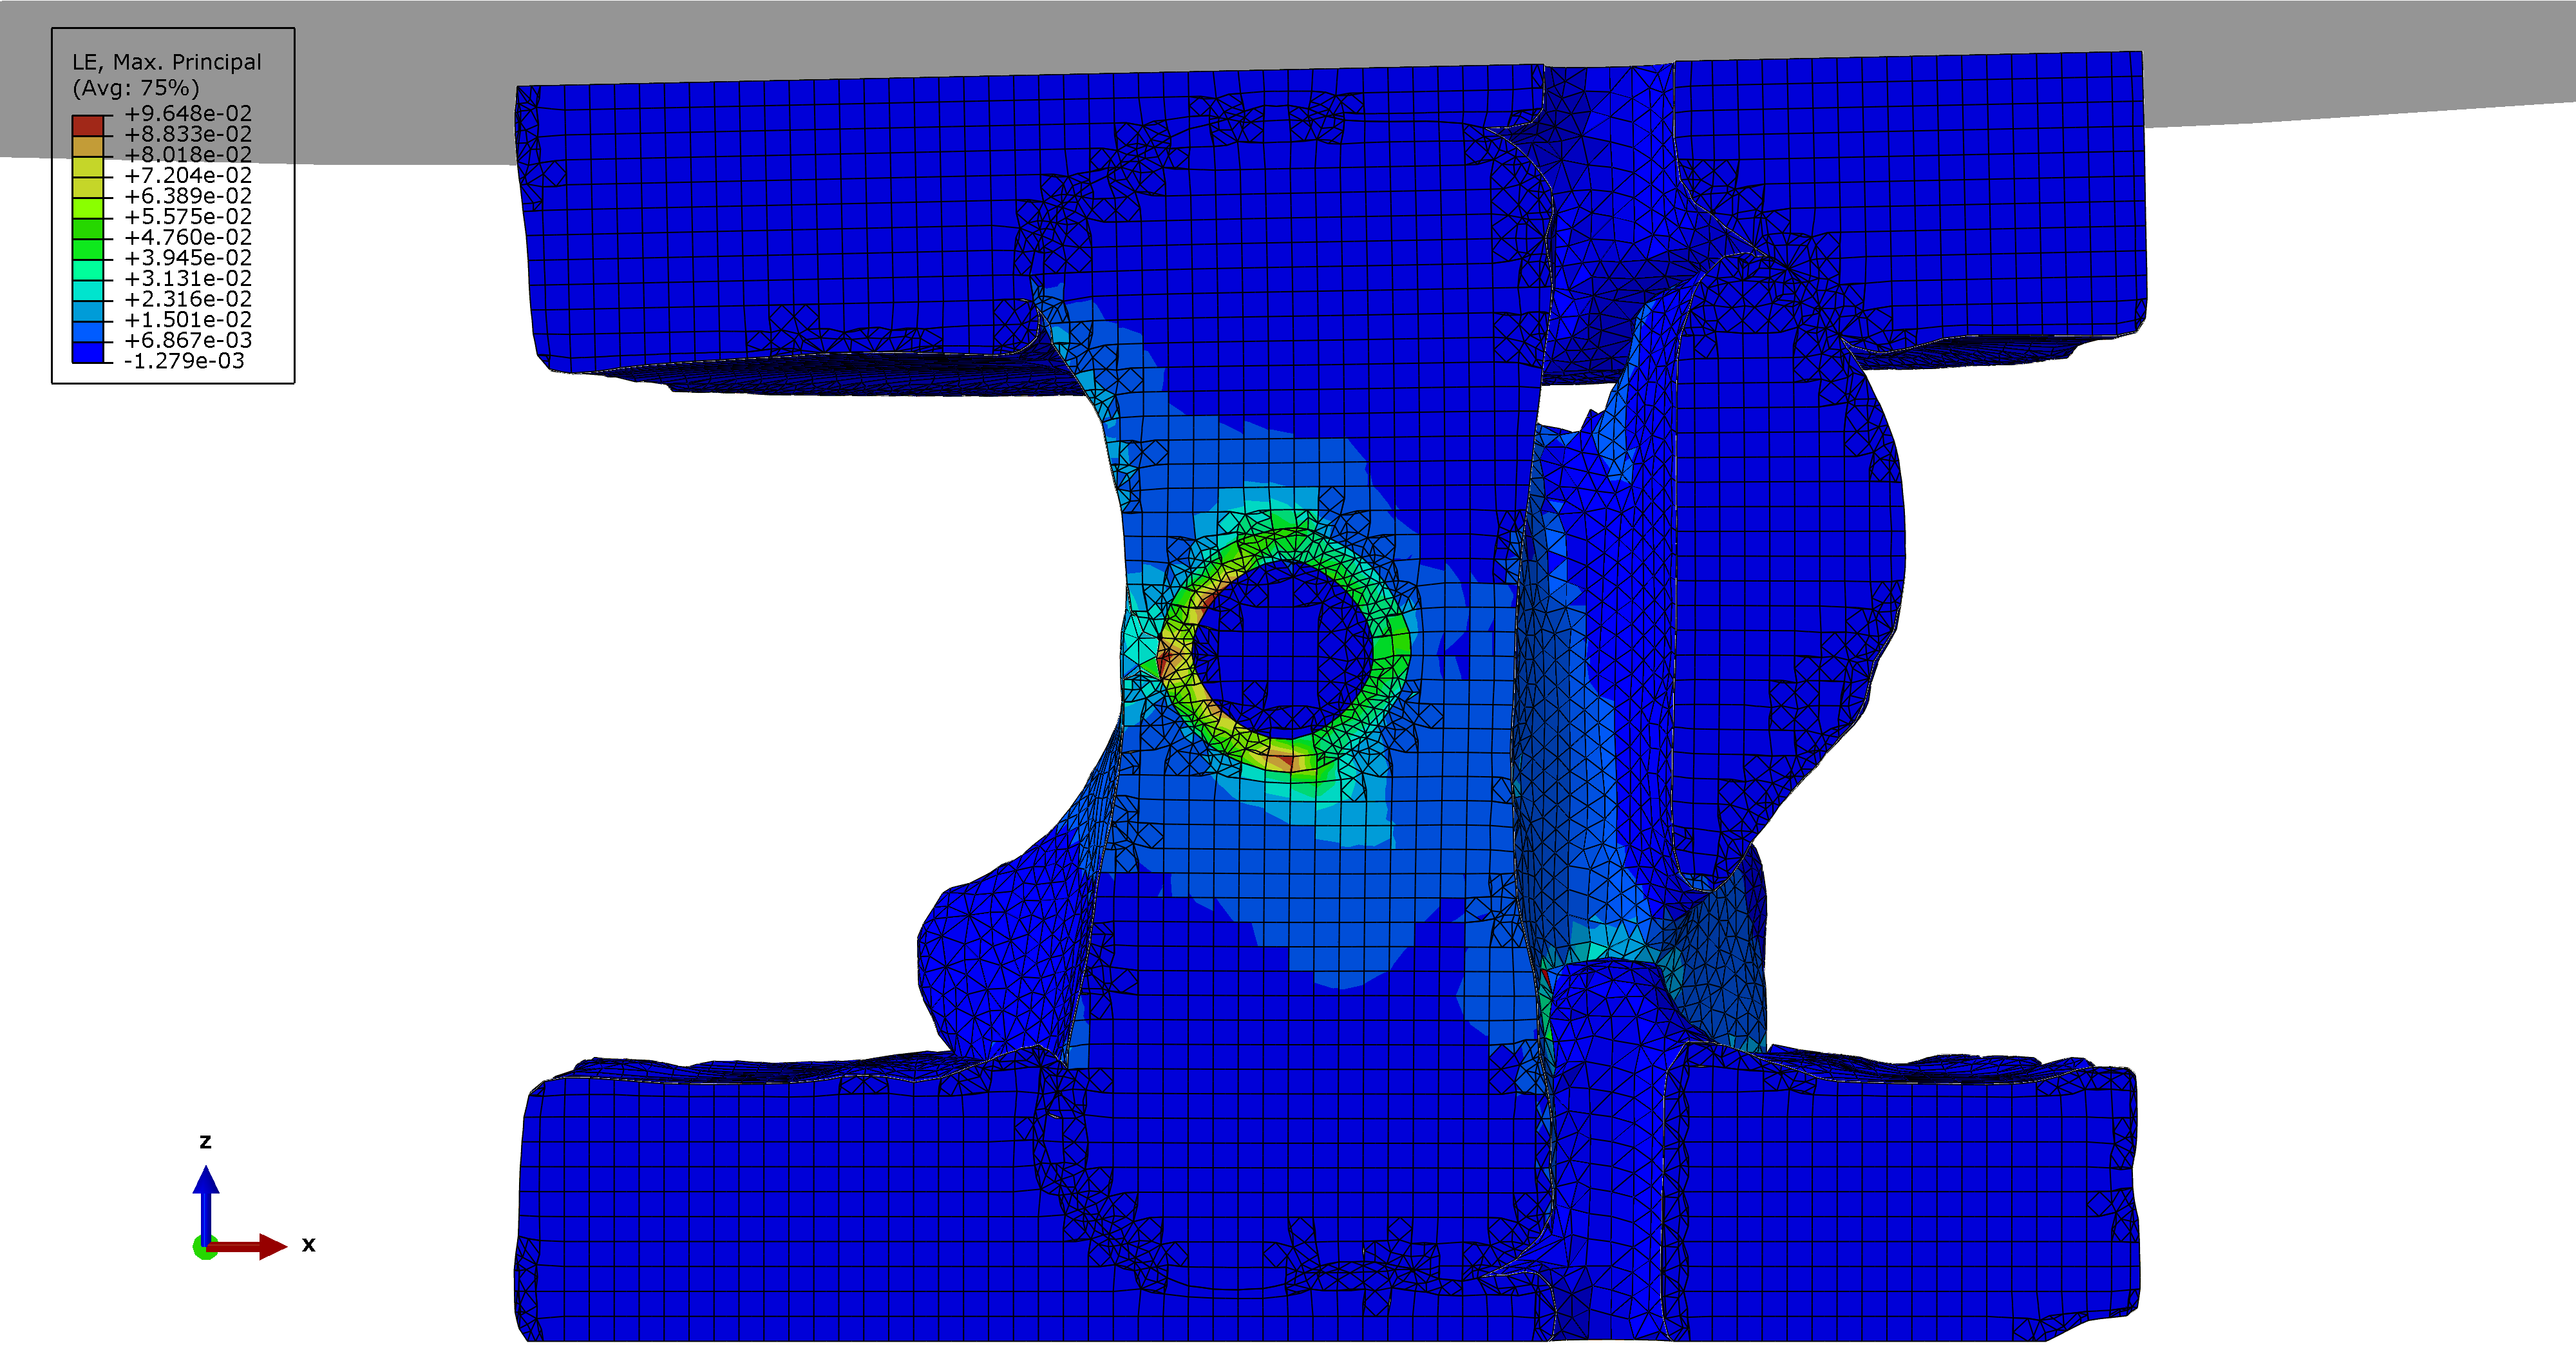
\includegraphics[width=10cm]{images/T2_CC2_intact_MM_cement_Anterior_ABAQUS_Strain.png}   & T2 CC2 \begin{itemize} \item  Computational:	2940 N/mm \item 4 \% Cement Fill \end{itemize} \\ \hline 
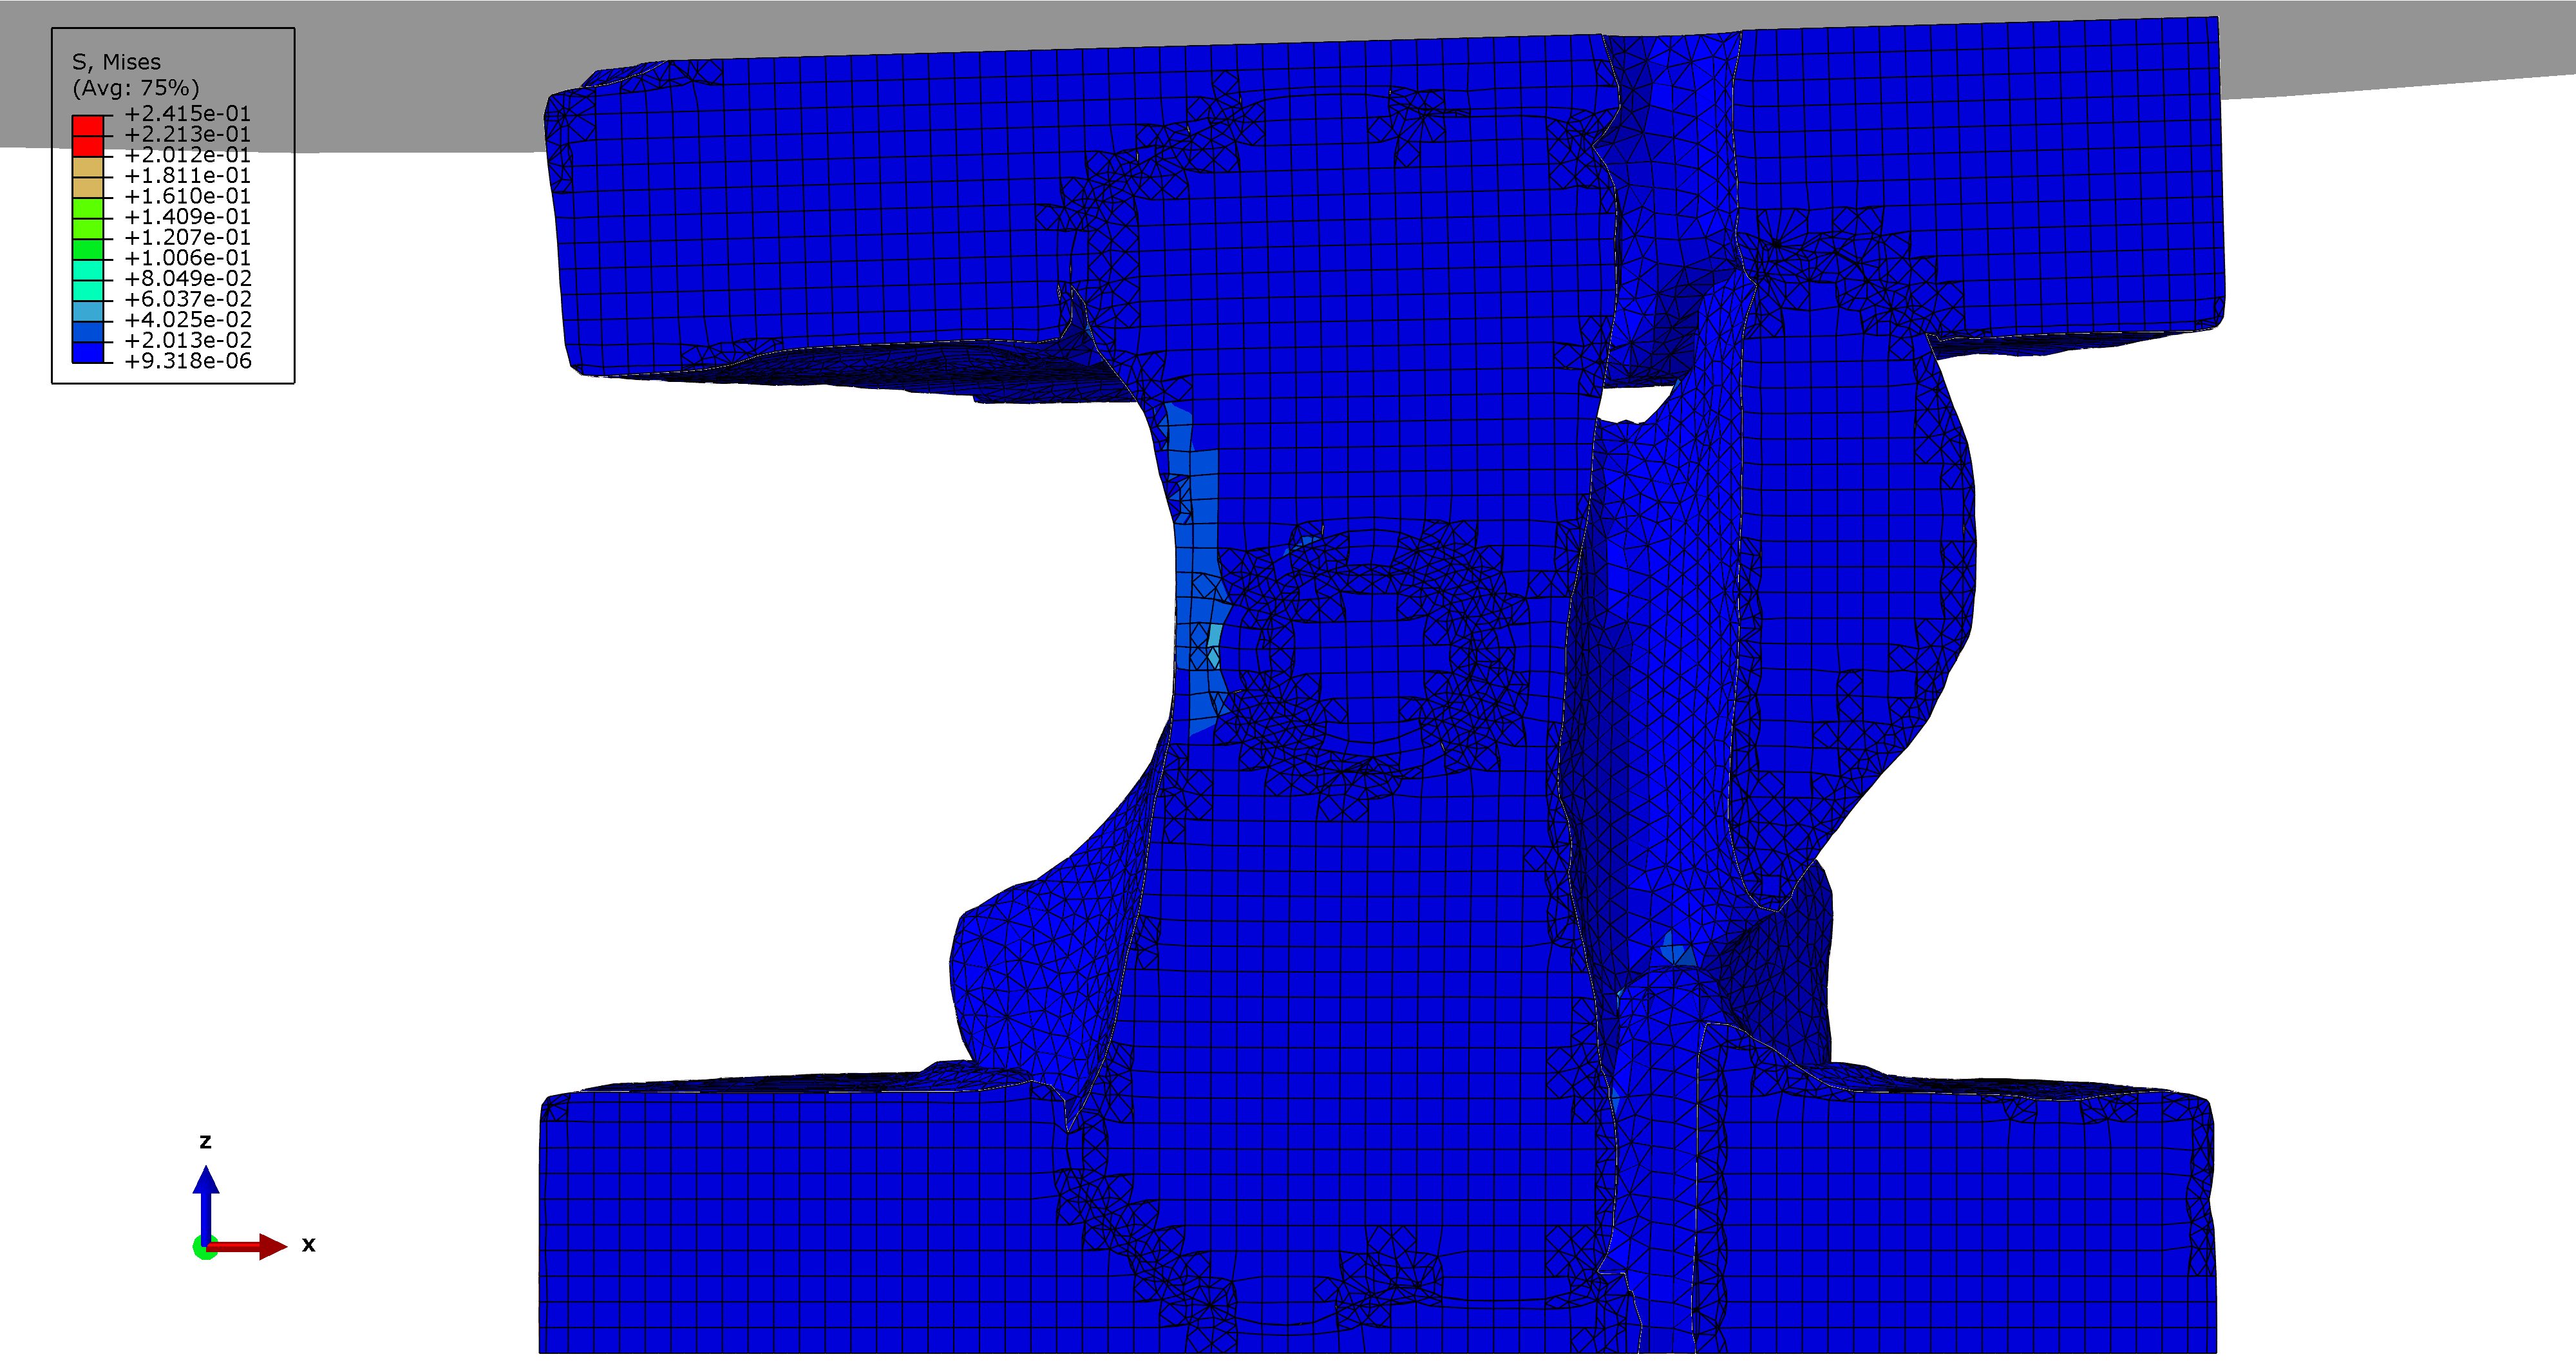
\includegraphics[width=10cm]{images/T2_CC2_intact_MM_cement_Middle_ABAQUS_Stress.png}   & 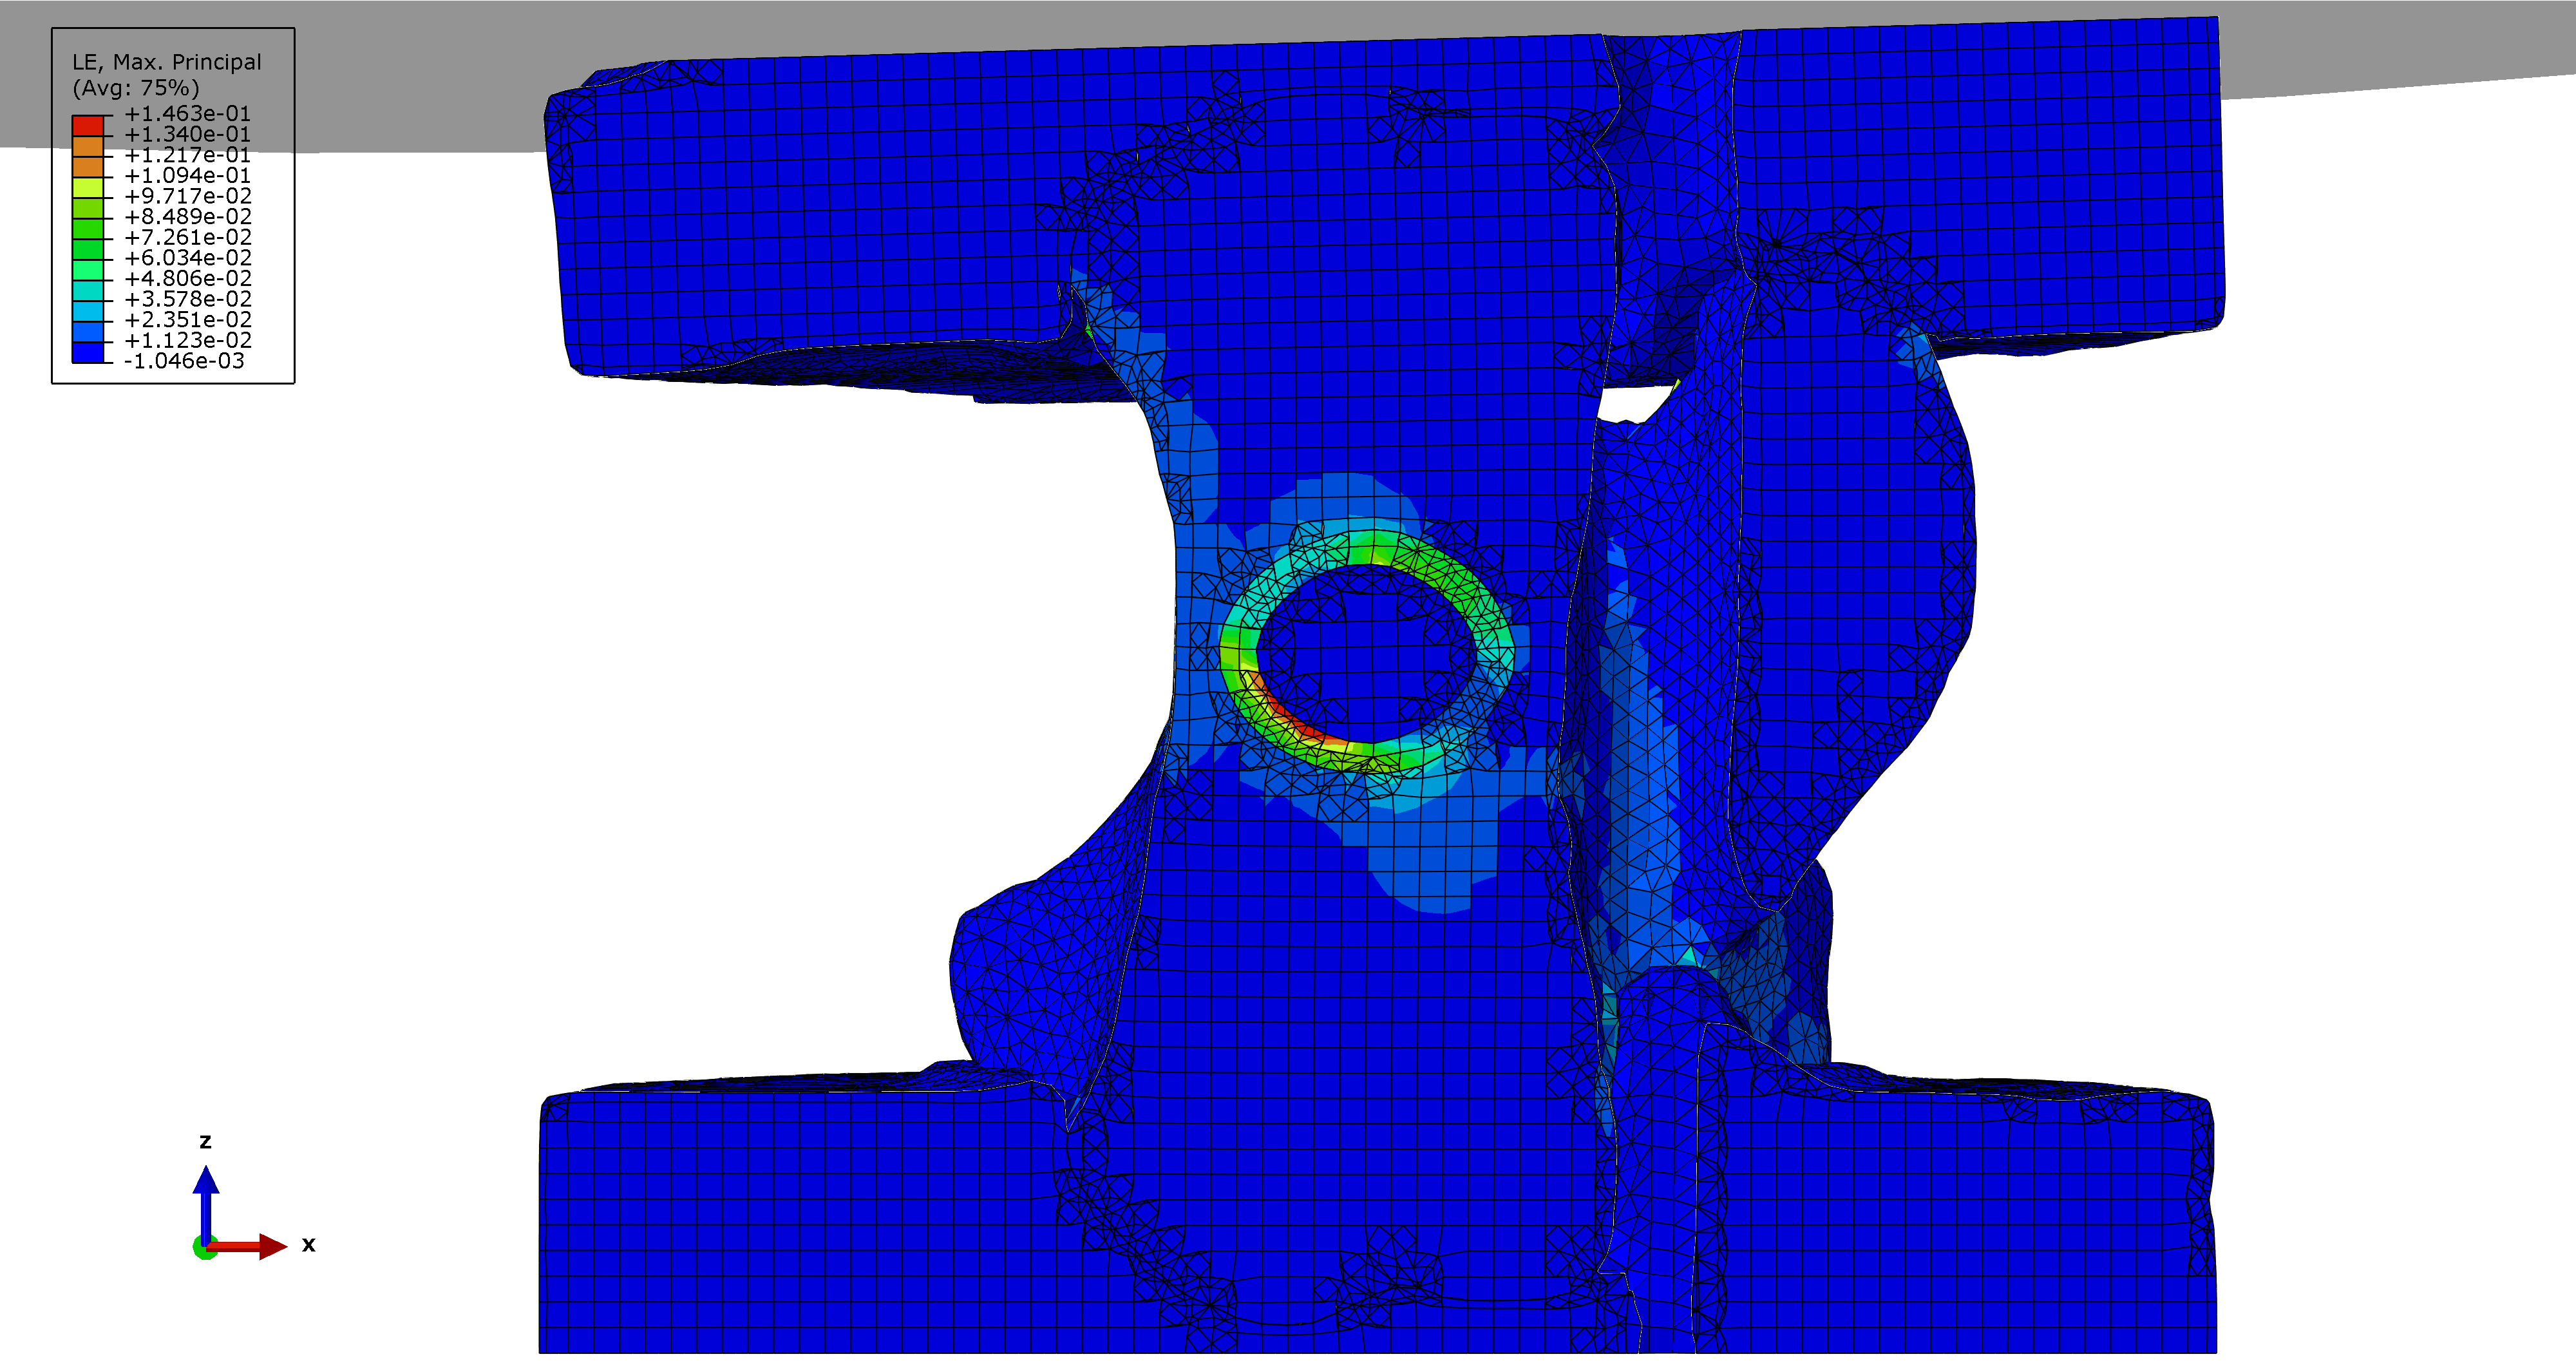
\includegraphics[width=10cm]{images/T2_CC2_intact_MM_cement_Middle_ABAQUS_Strain.png}   & T2 CC2 \begin{itemize} \item  Computational:	2664 N/mm \item 4 \% Cement Fill \end{itemize} \\ \hline 
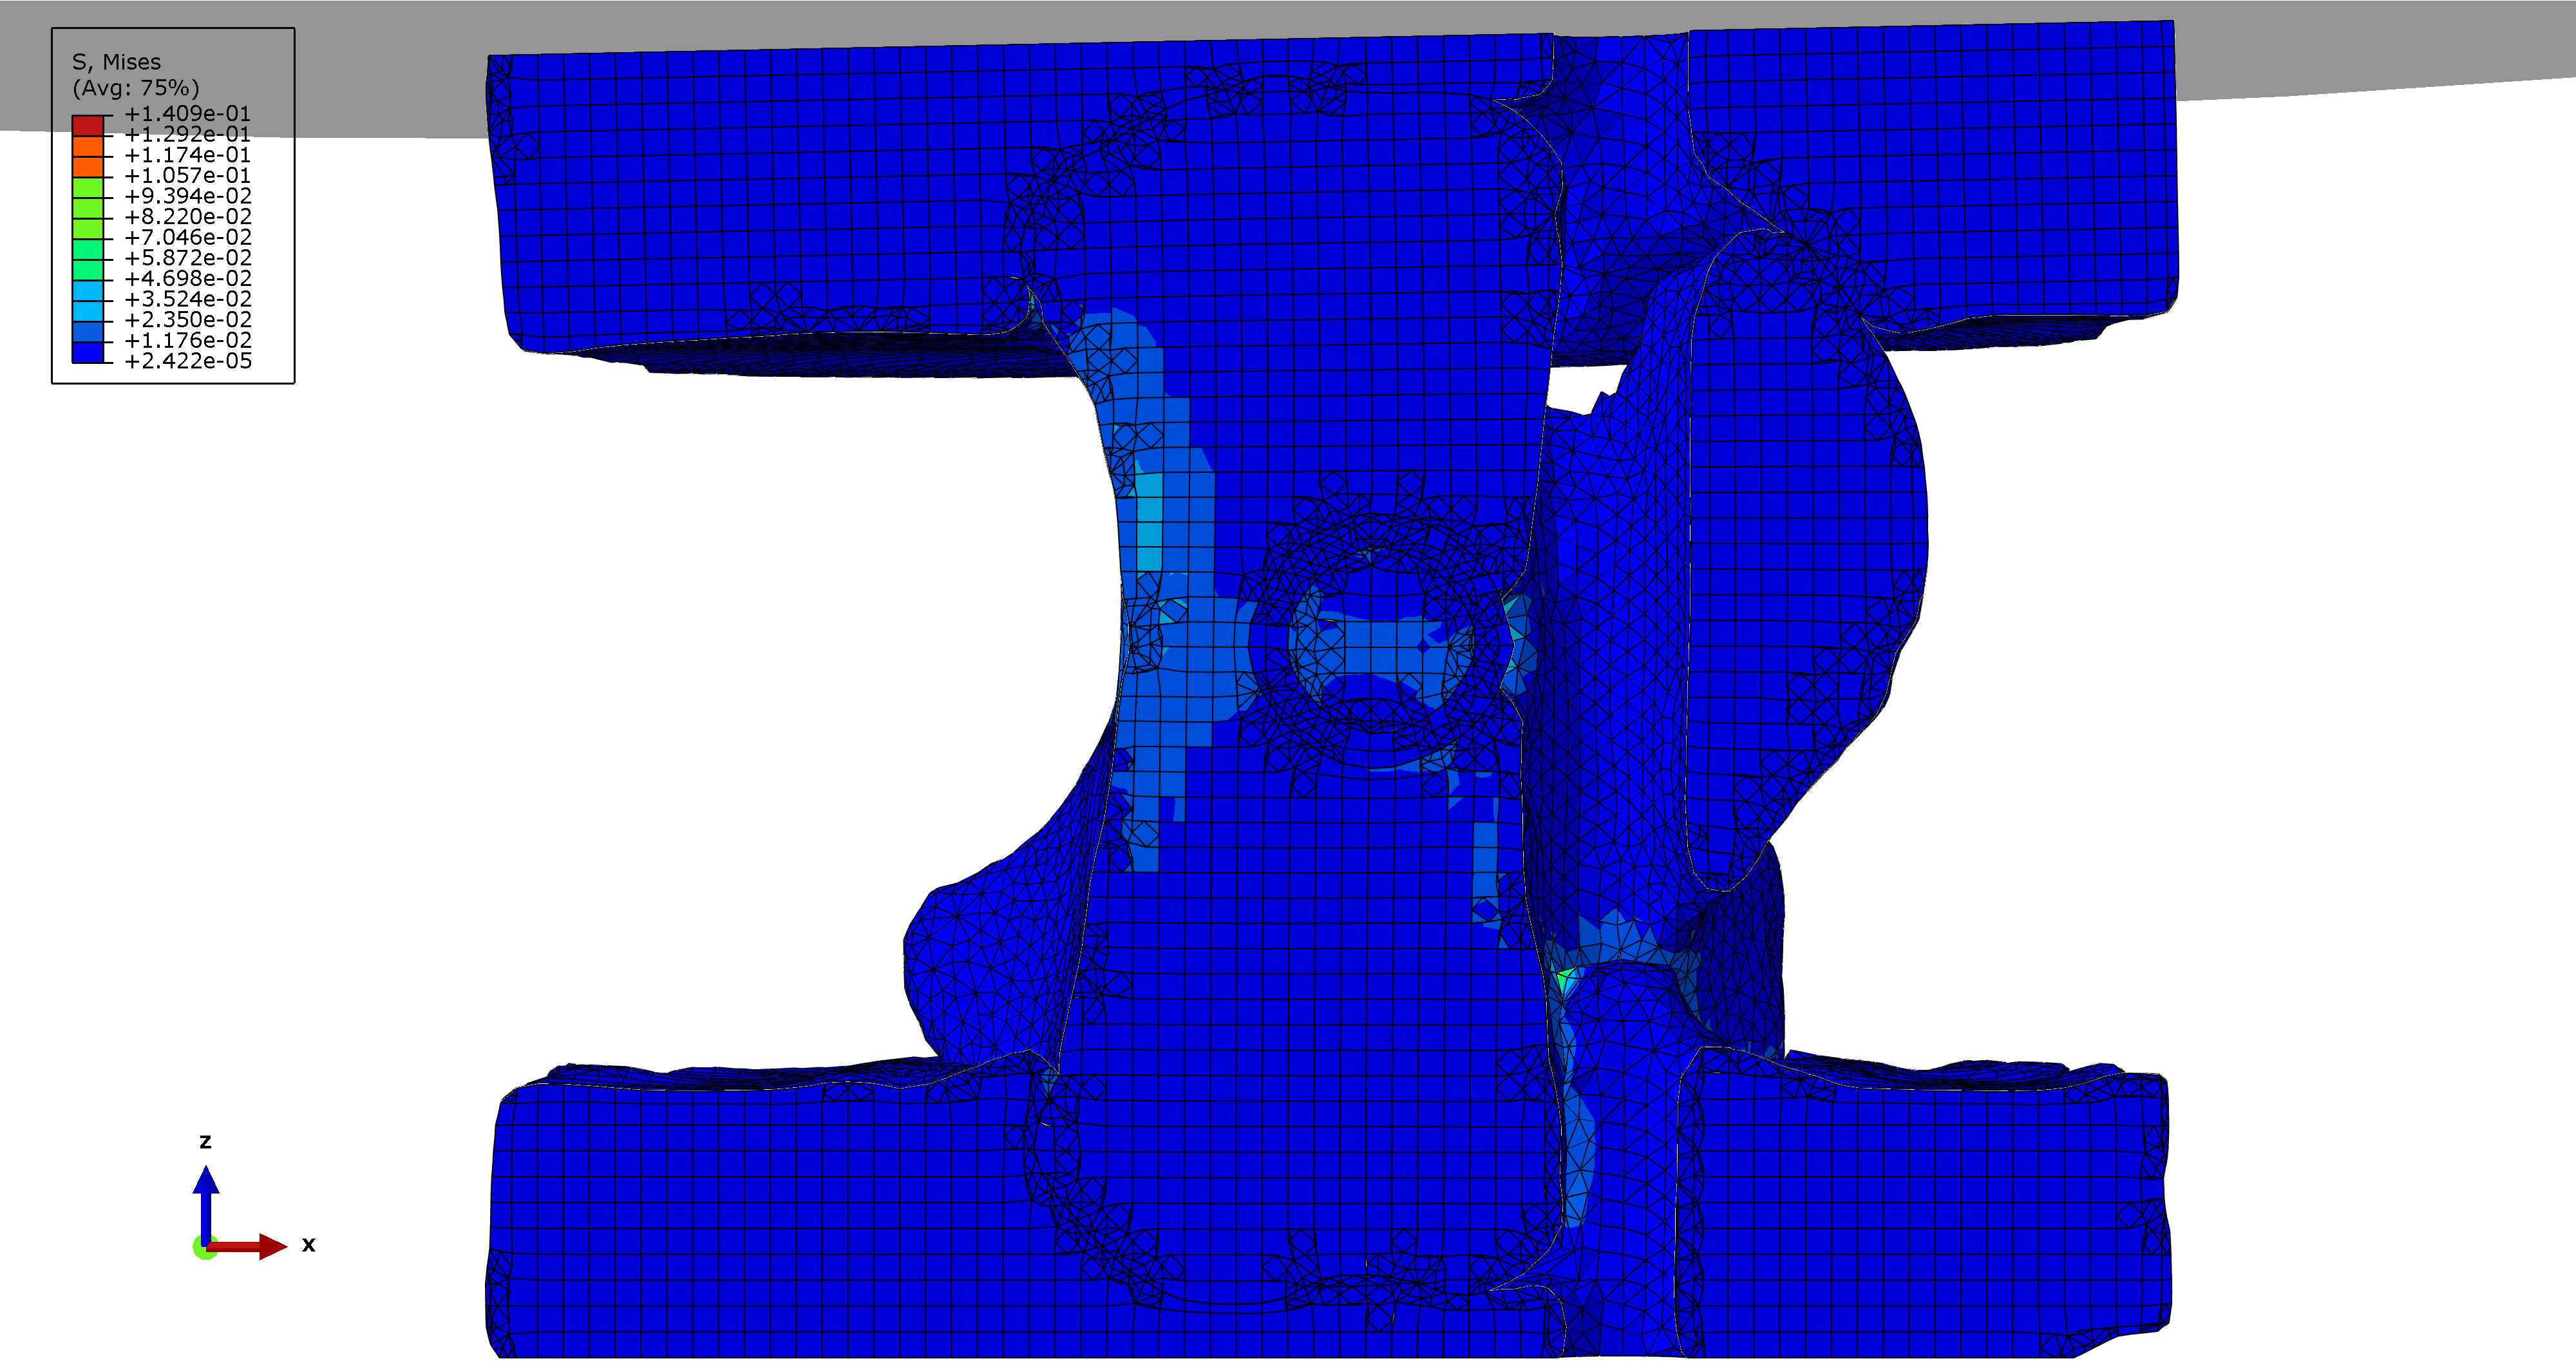
\includegraphics[width=10cm]{images/T2_CC2_intact_MM_cement_Posterior_ABAQUS_Stress.png}   & 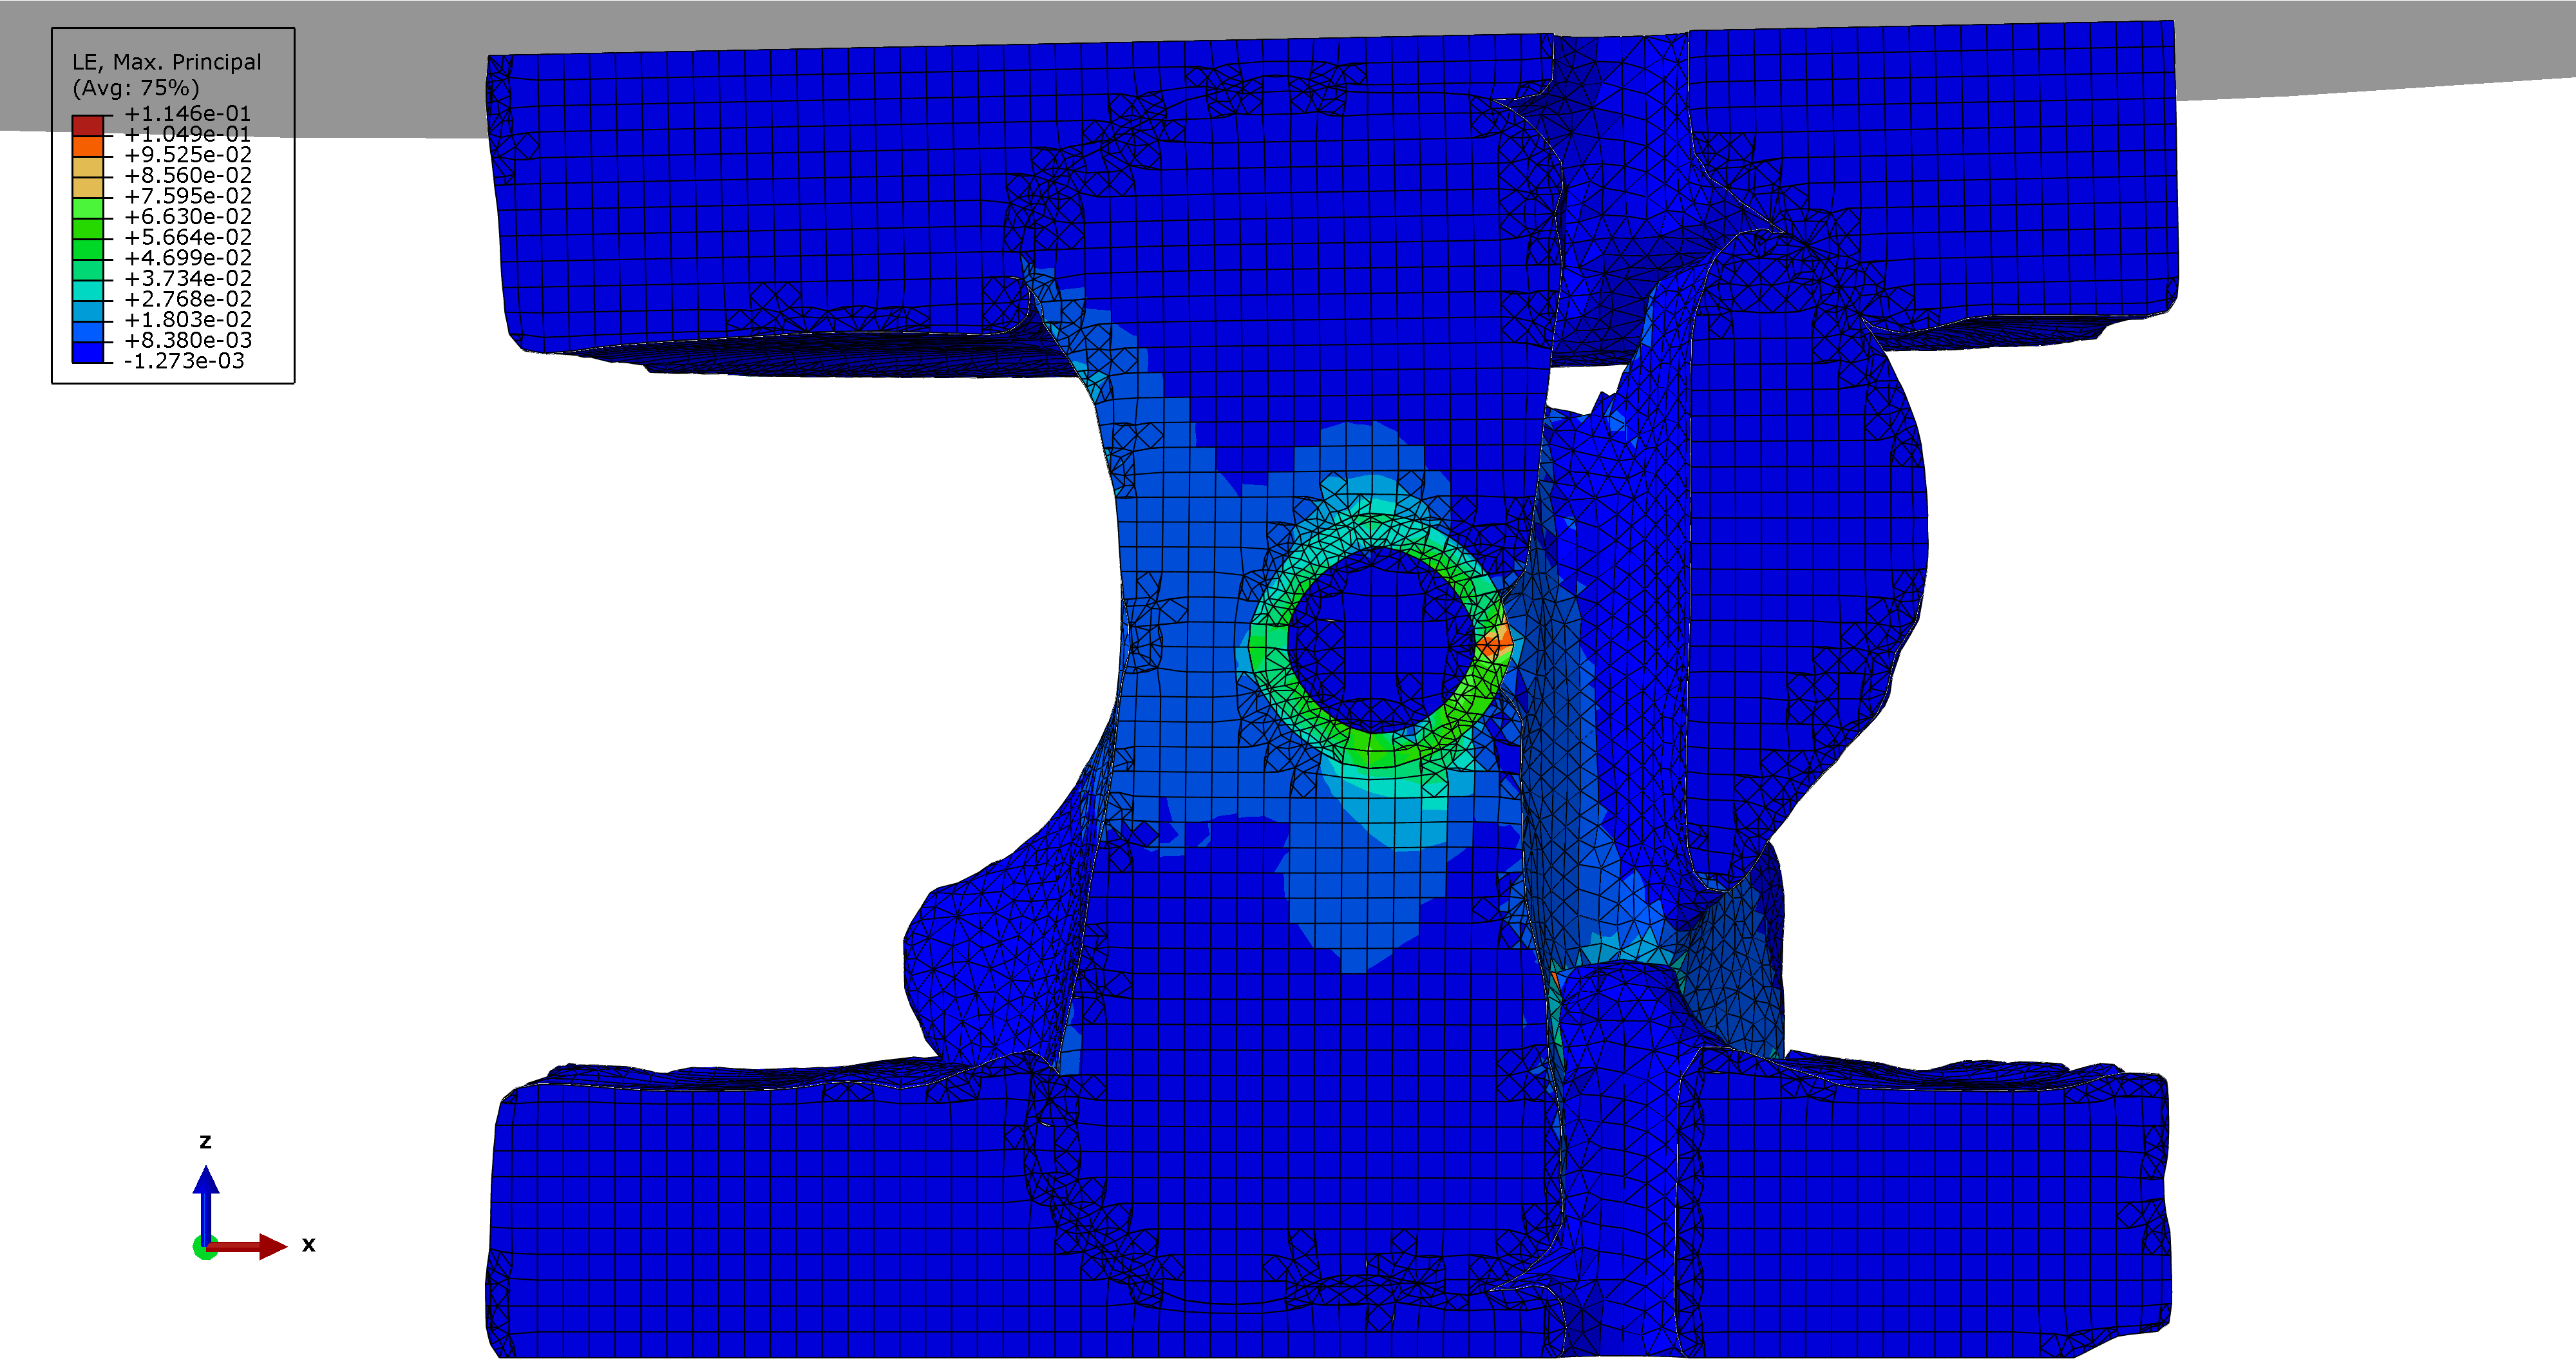
\includegraphics[width=10cm]{images/T2_CC2_intact_MM_cement_Posterior_ABAQUS_Strain.png}   & T2 CC2 \begin{itemize} \item  Computational:	3790  N/mm \end{itemize} \\ \hline 
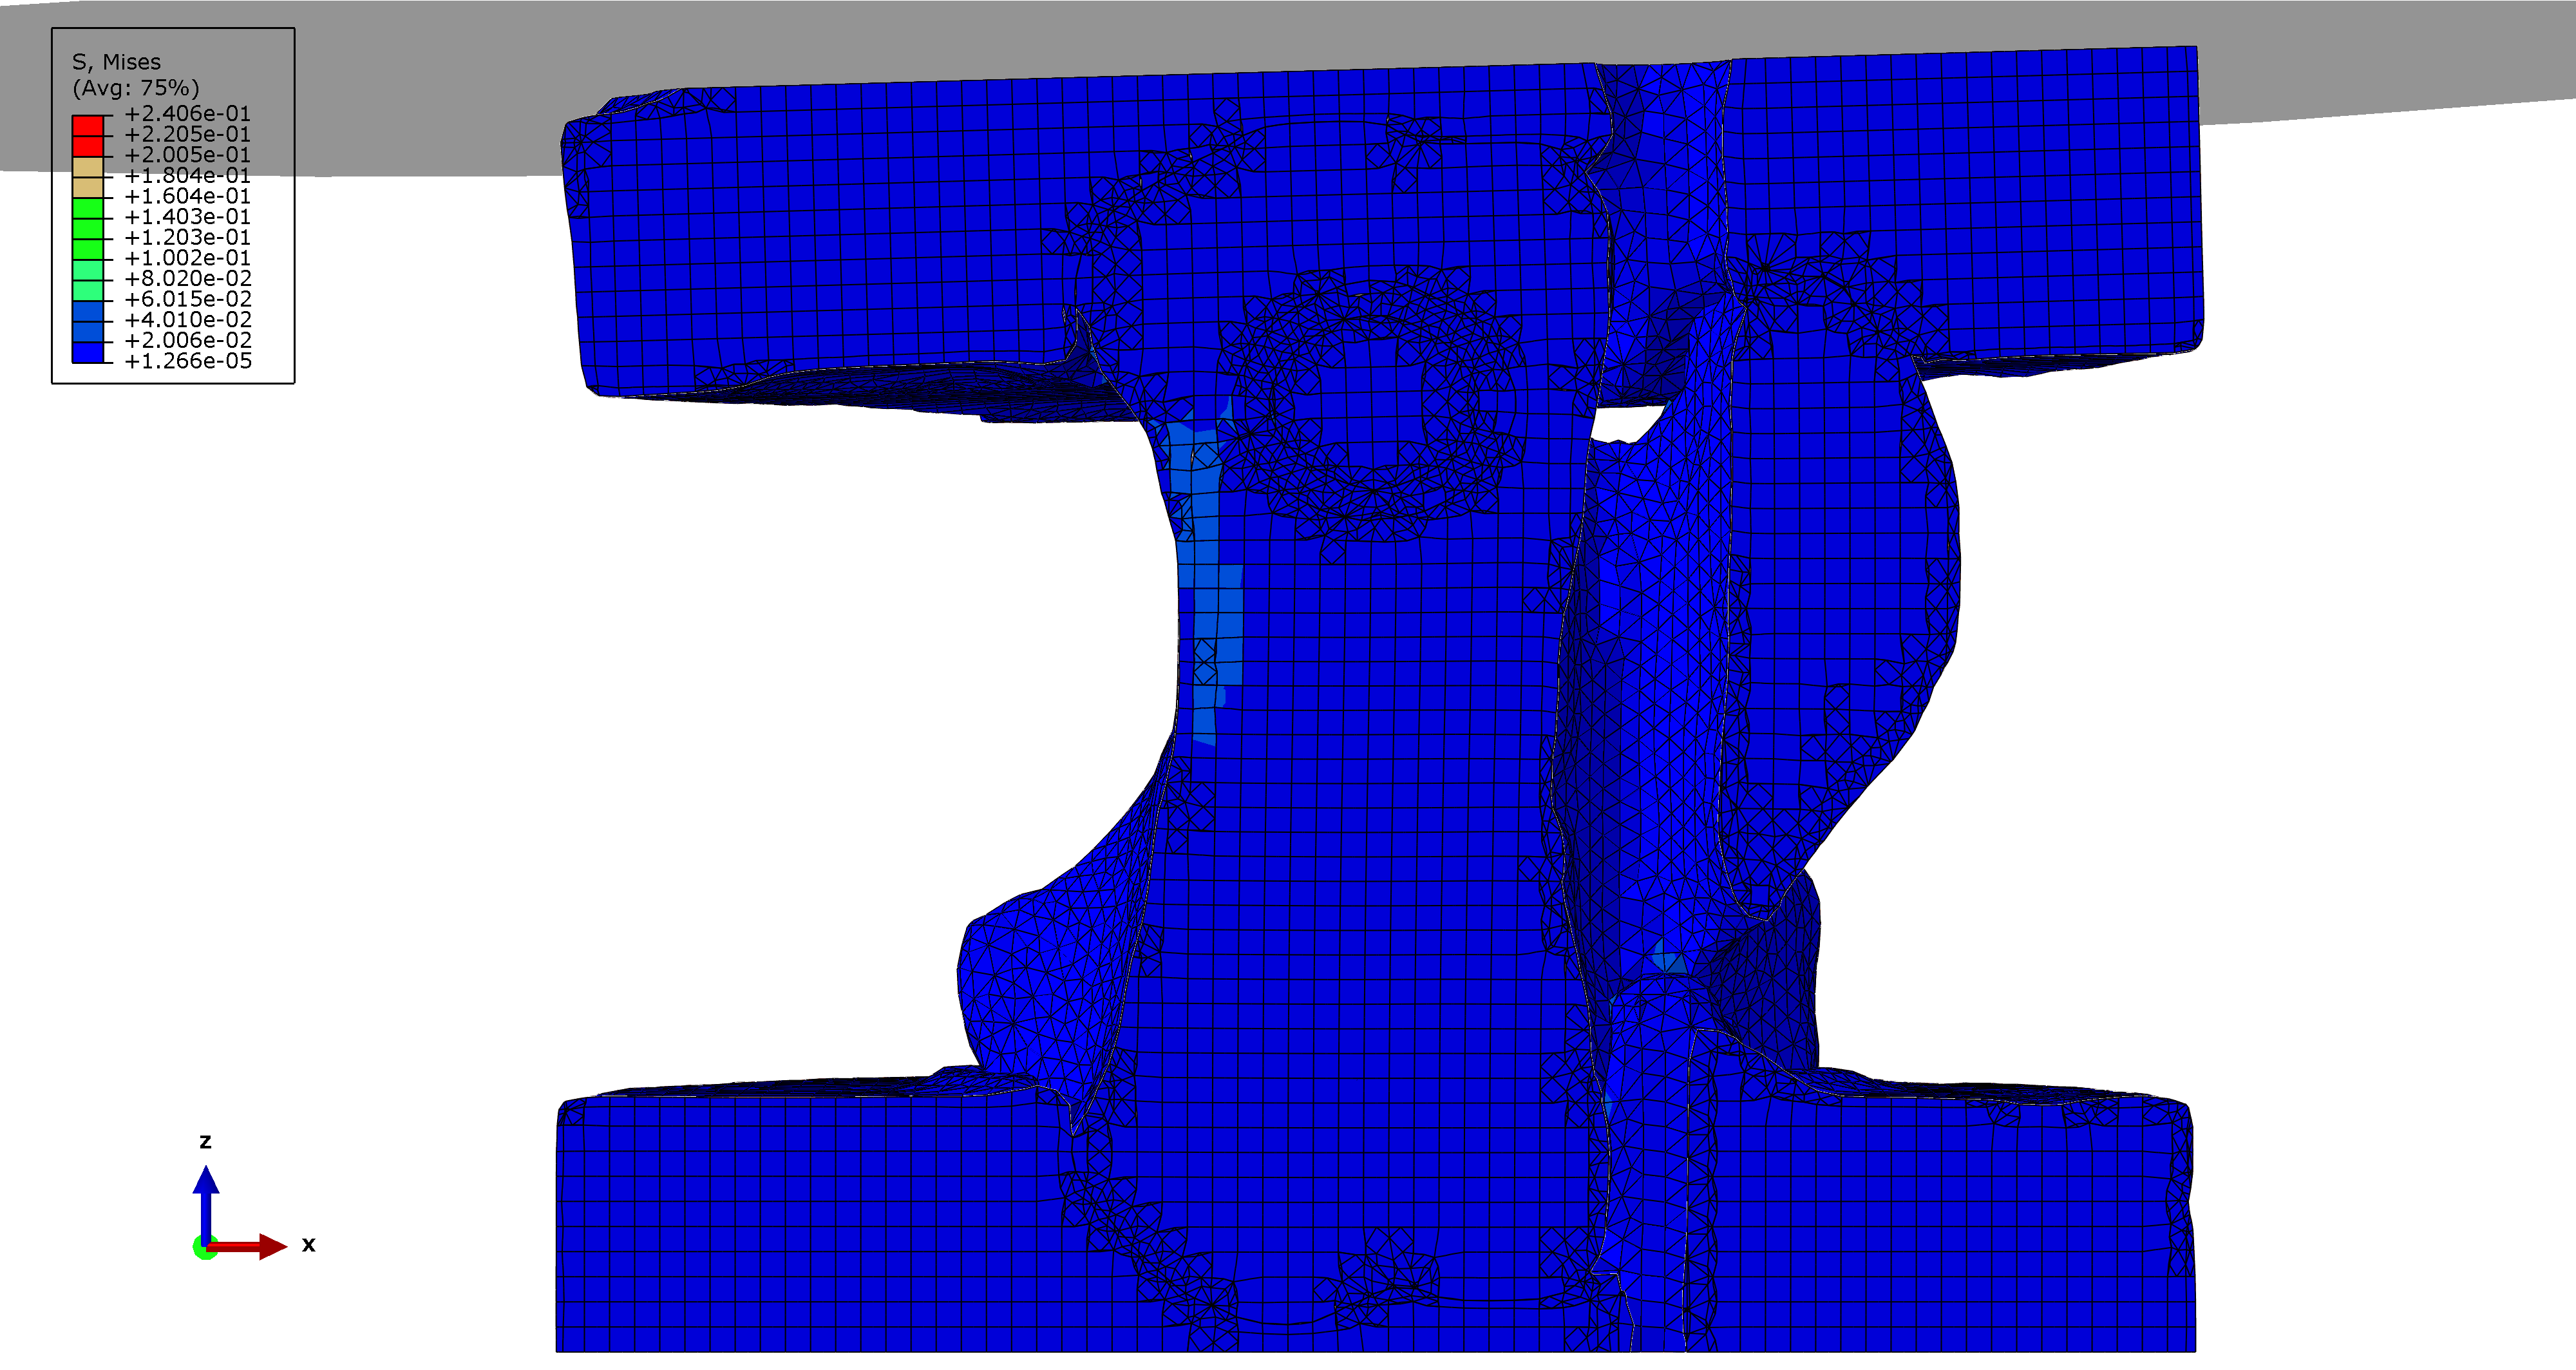
\includegraphics[width=10cm]{images/T2_CC2_intact_MM_cement_Top_ABAQUS_Stress.png}   & 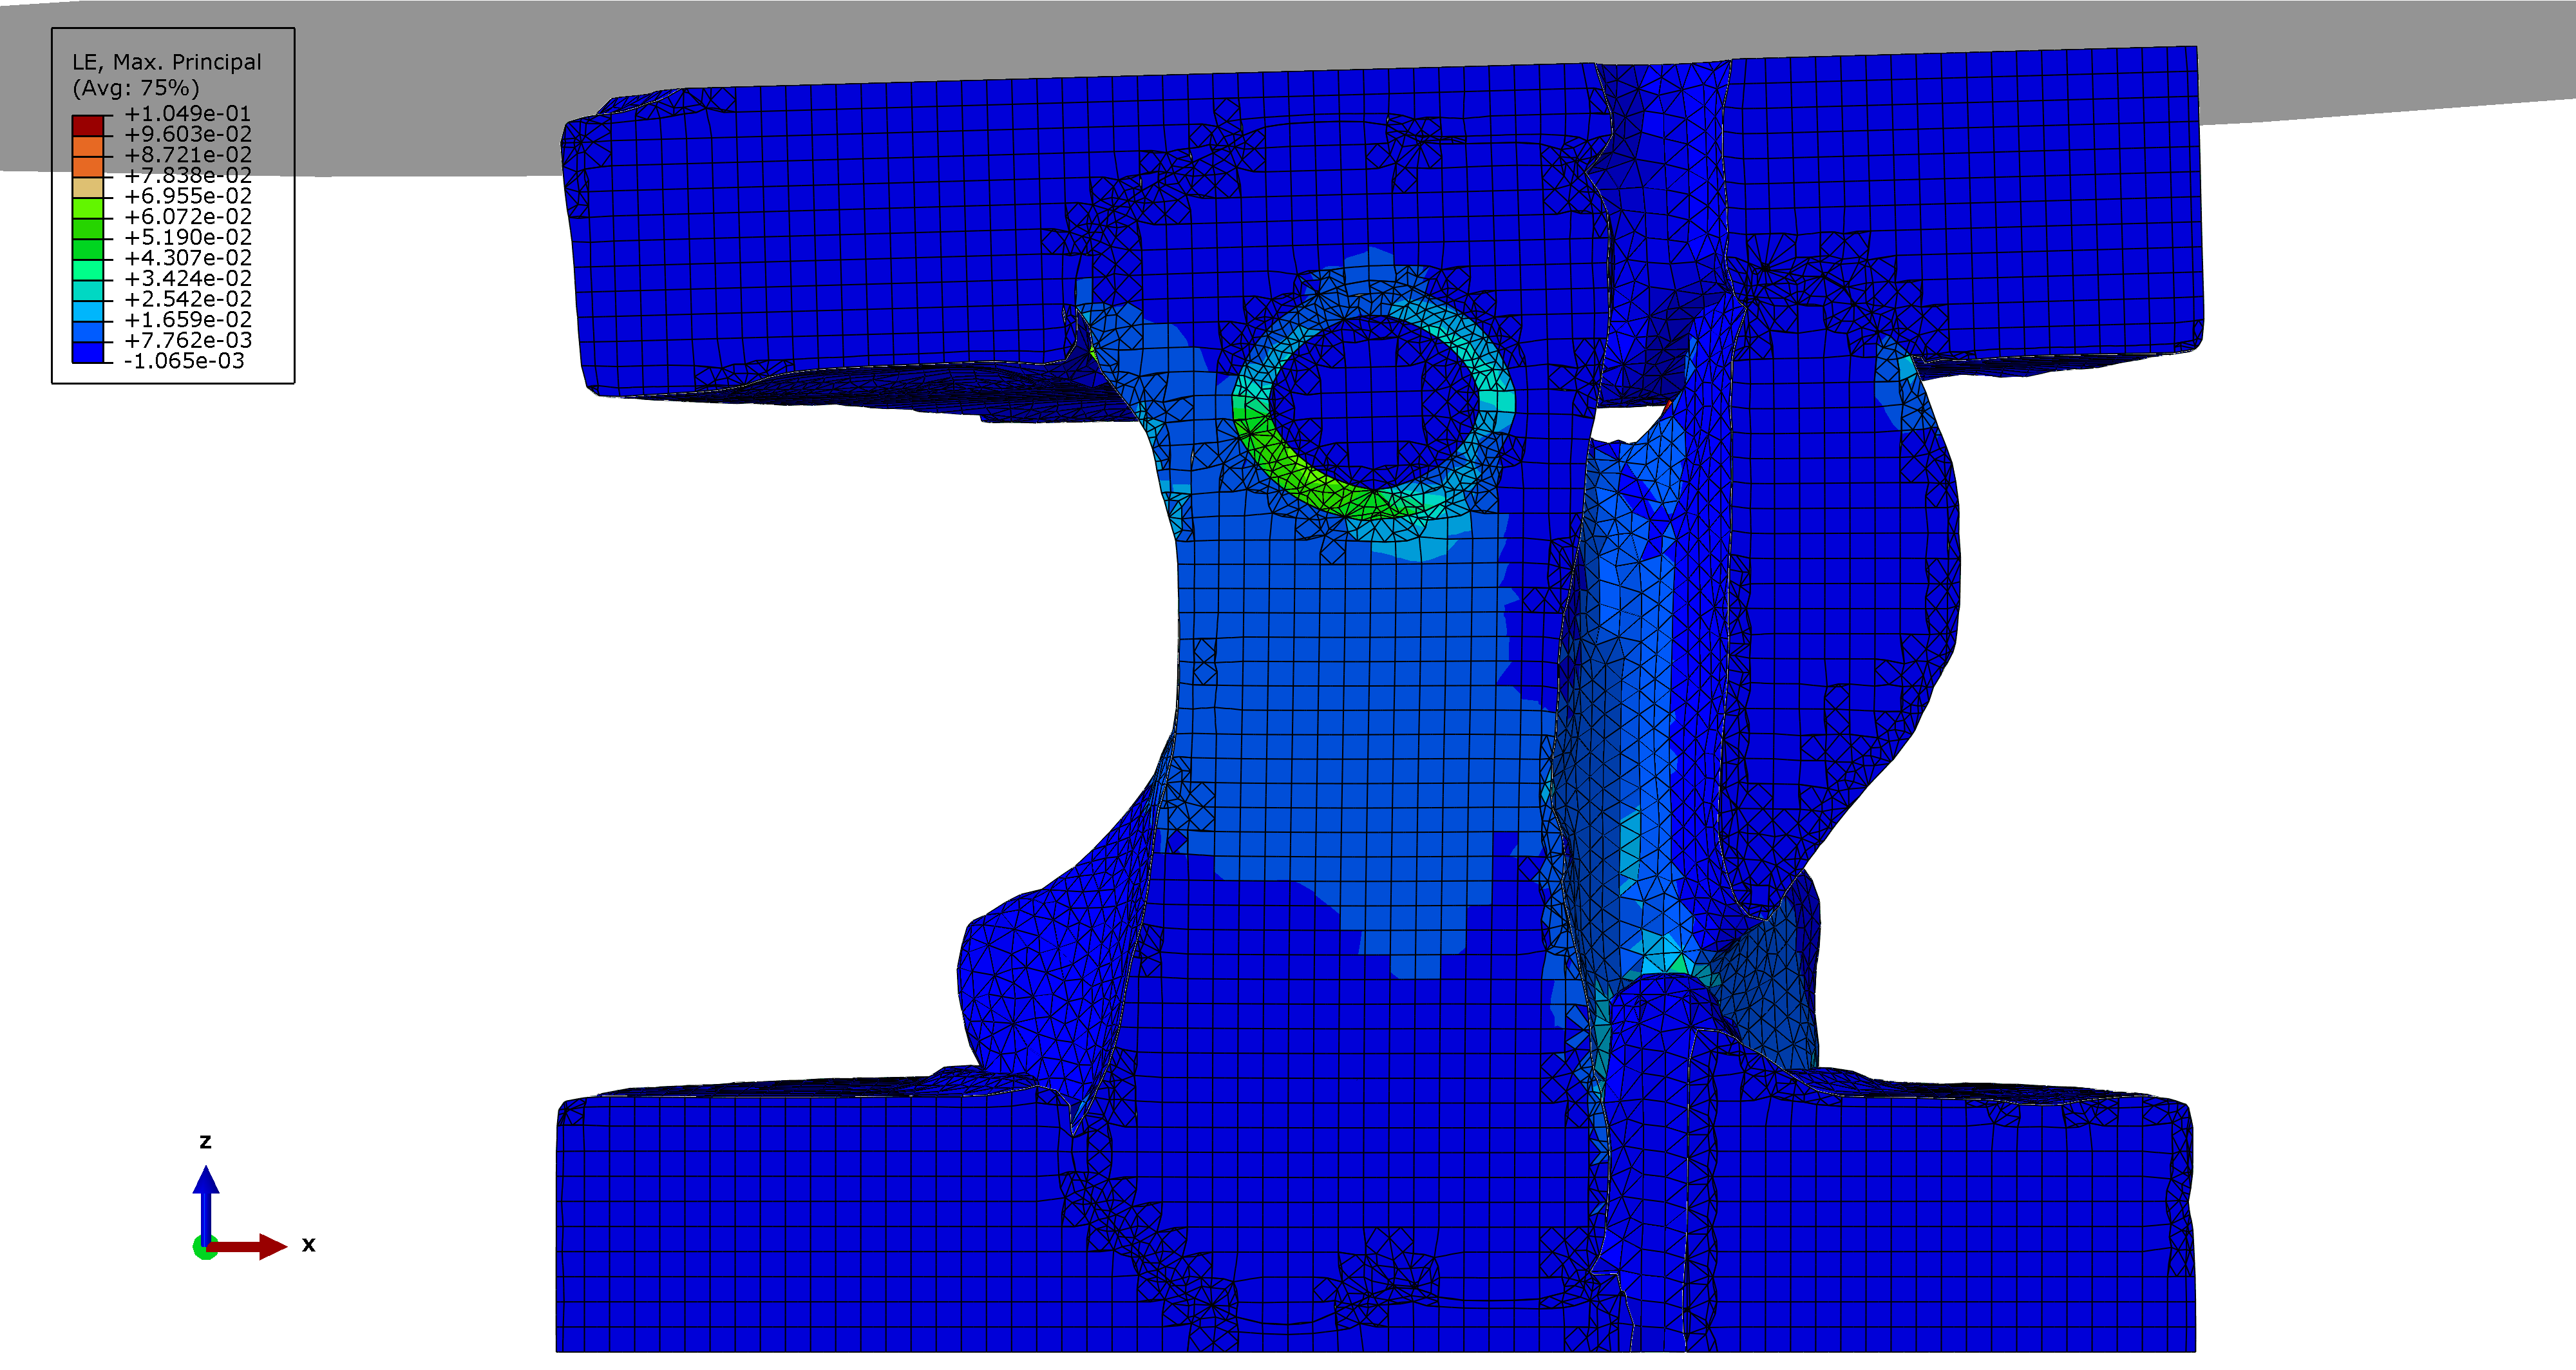
\includegraphics[width=10cm]{images/T2_CC2_intact_MM_cement_Top_ABAQUS_Strain.png}   & T2 CC2 \begin{itemize} \item  Computational:	4370  N/mm \item 4 \% Cement Fill \end{itemize} \\ \hline 
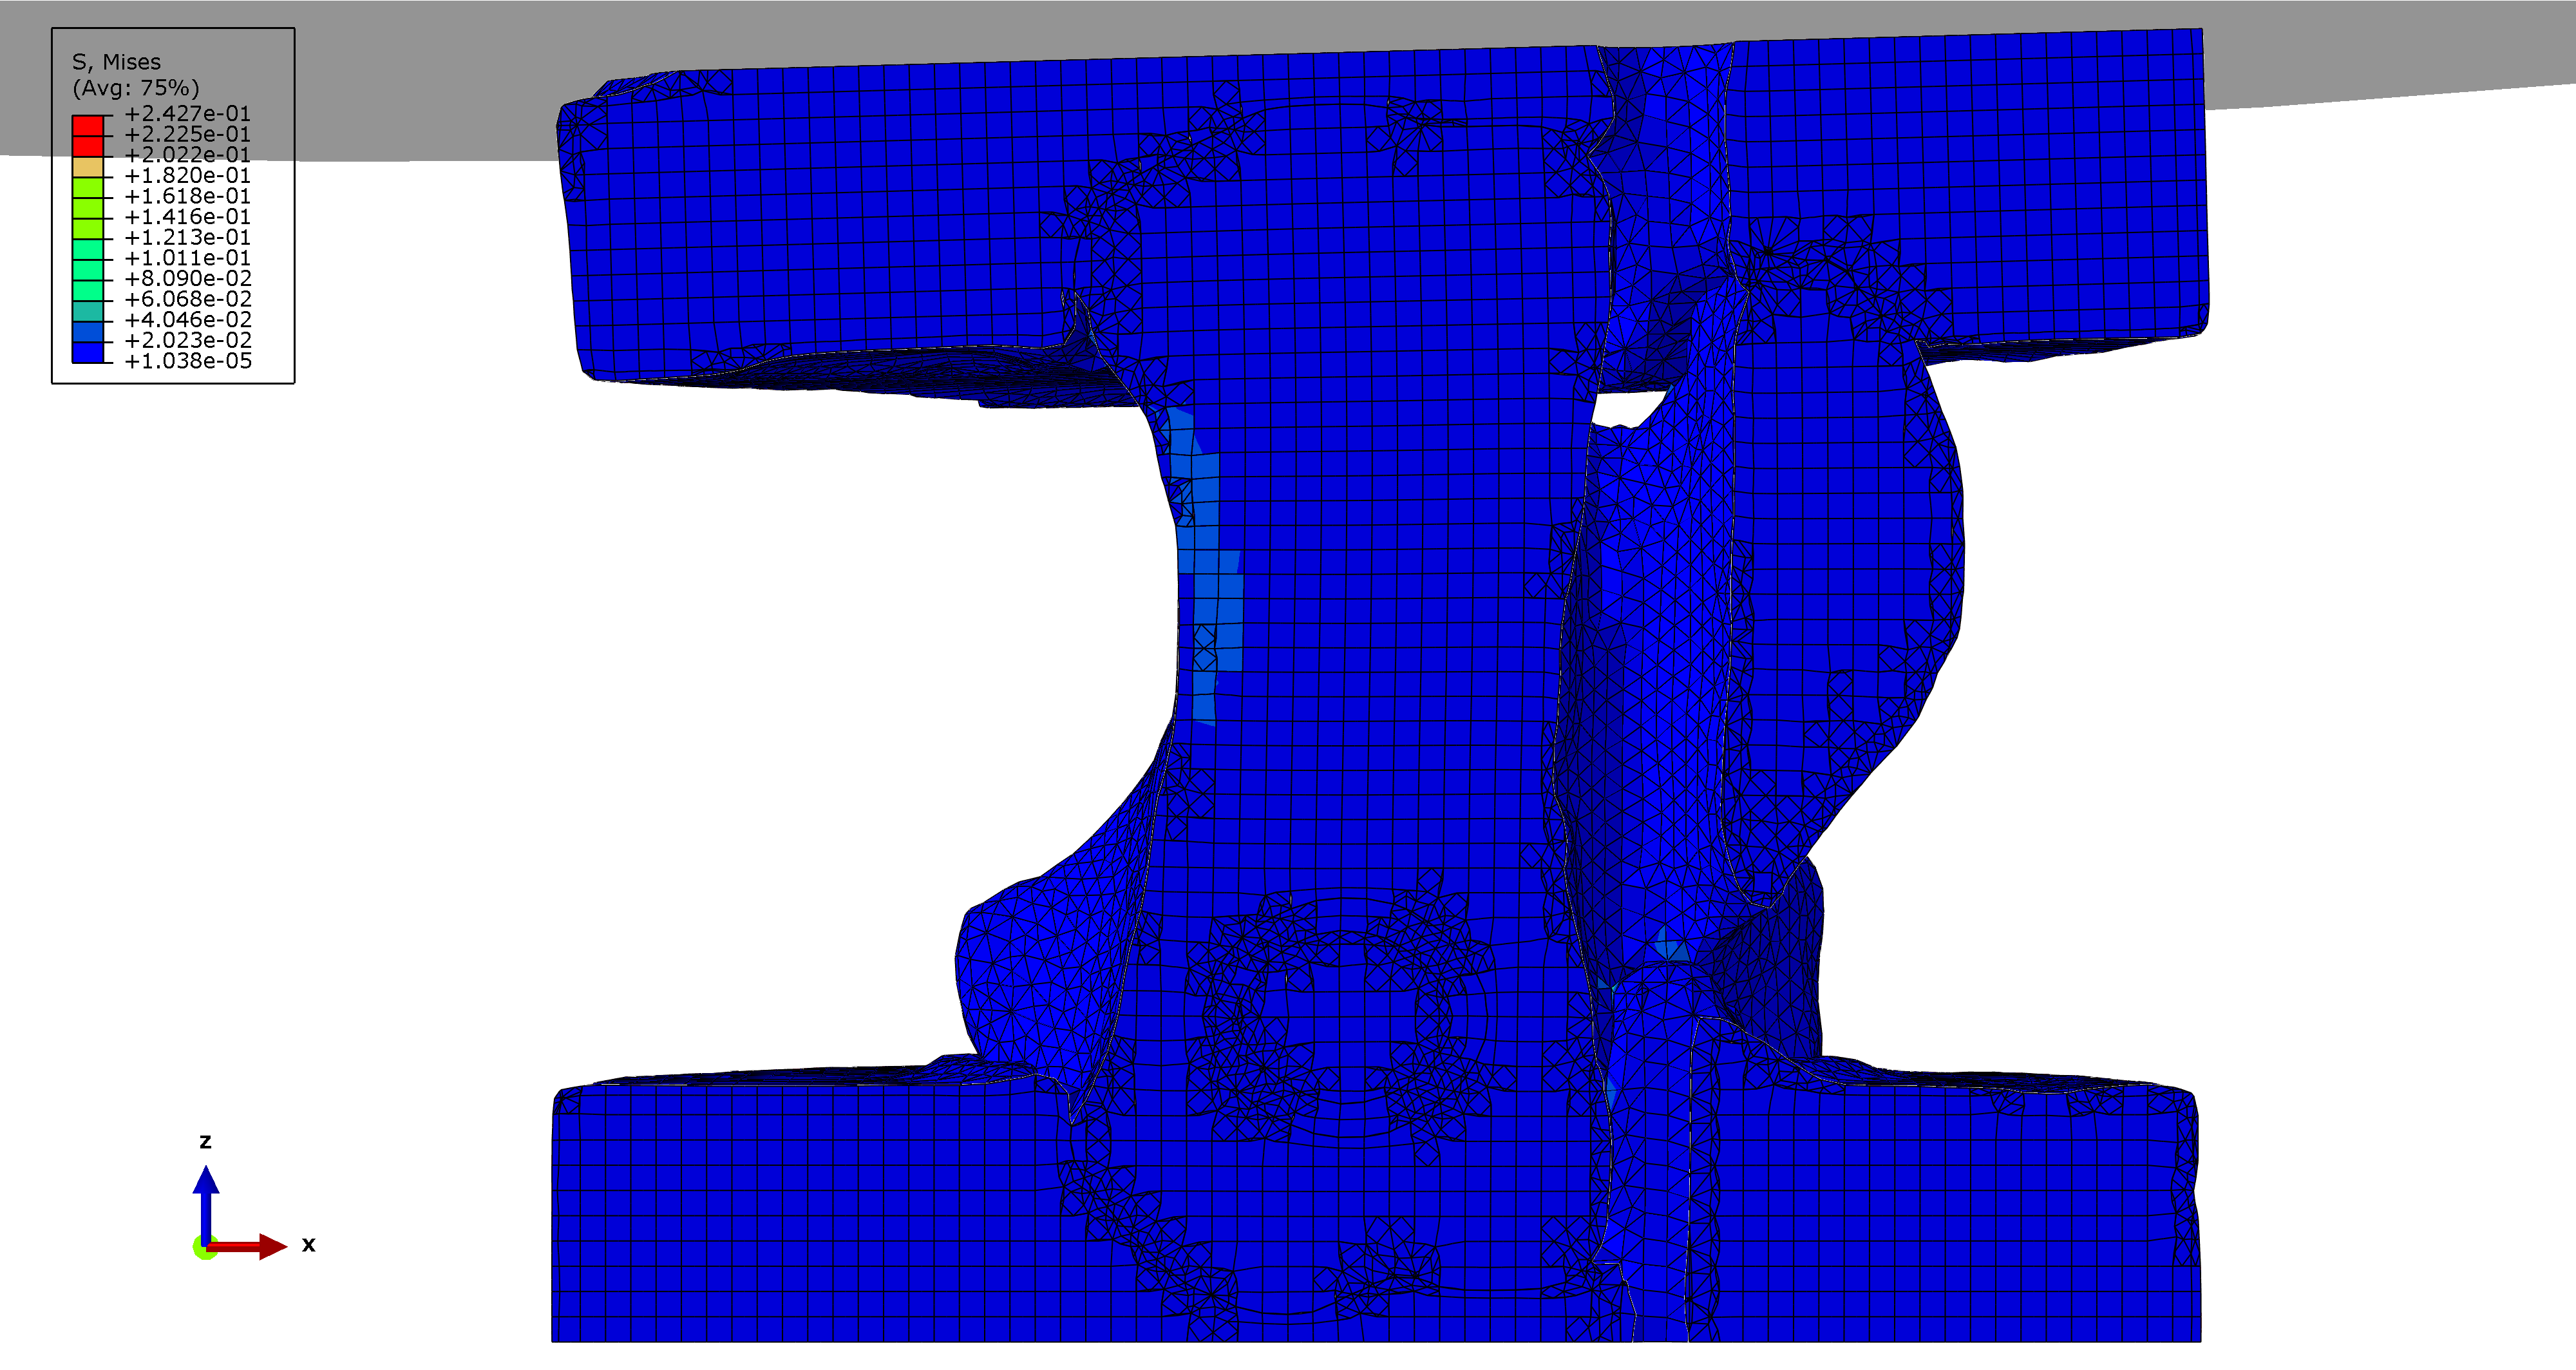
\includegraphics[width=10cm]{images/T2_CC2_intact_MM_cement_Bottom_ABAQUS_Stress.png}   & 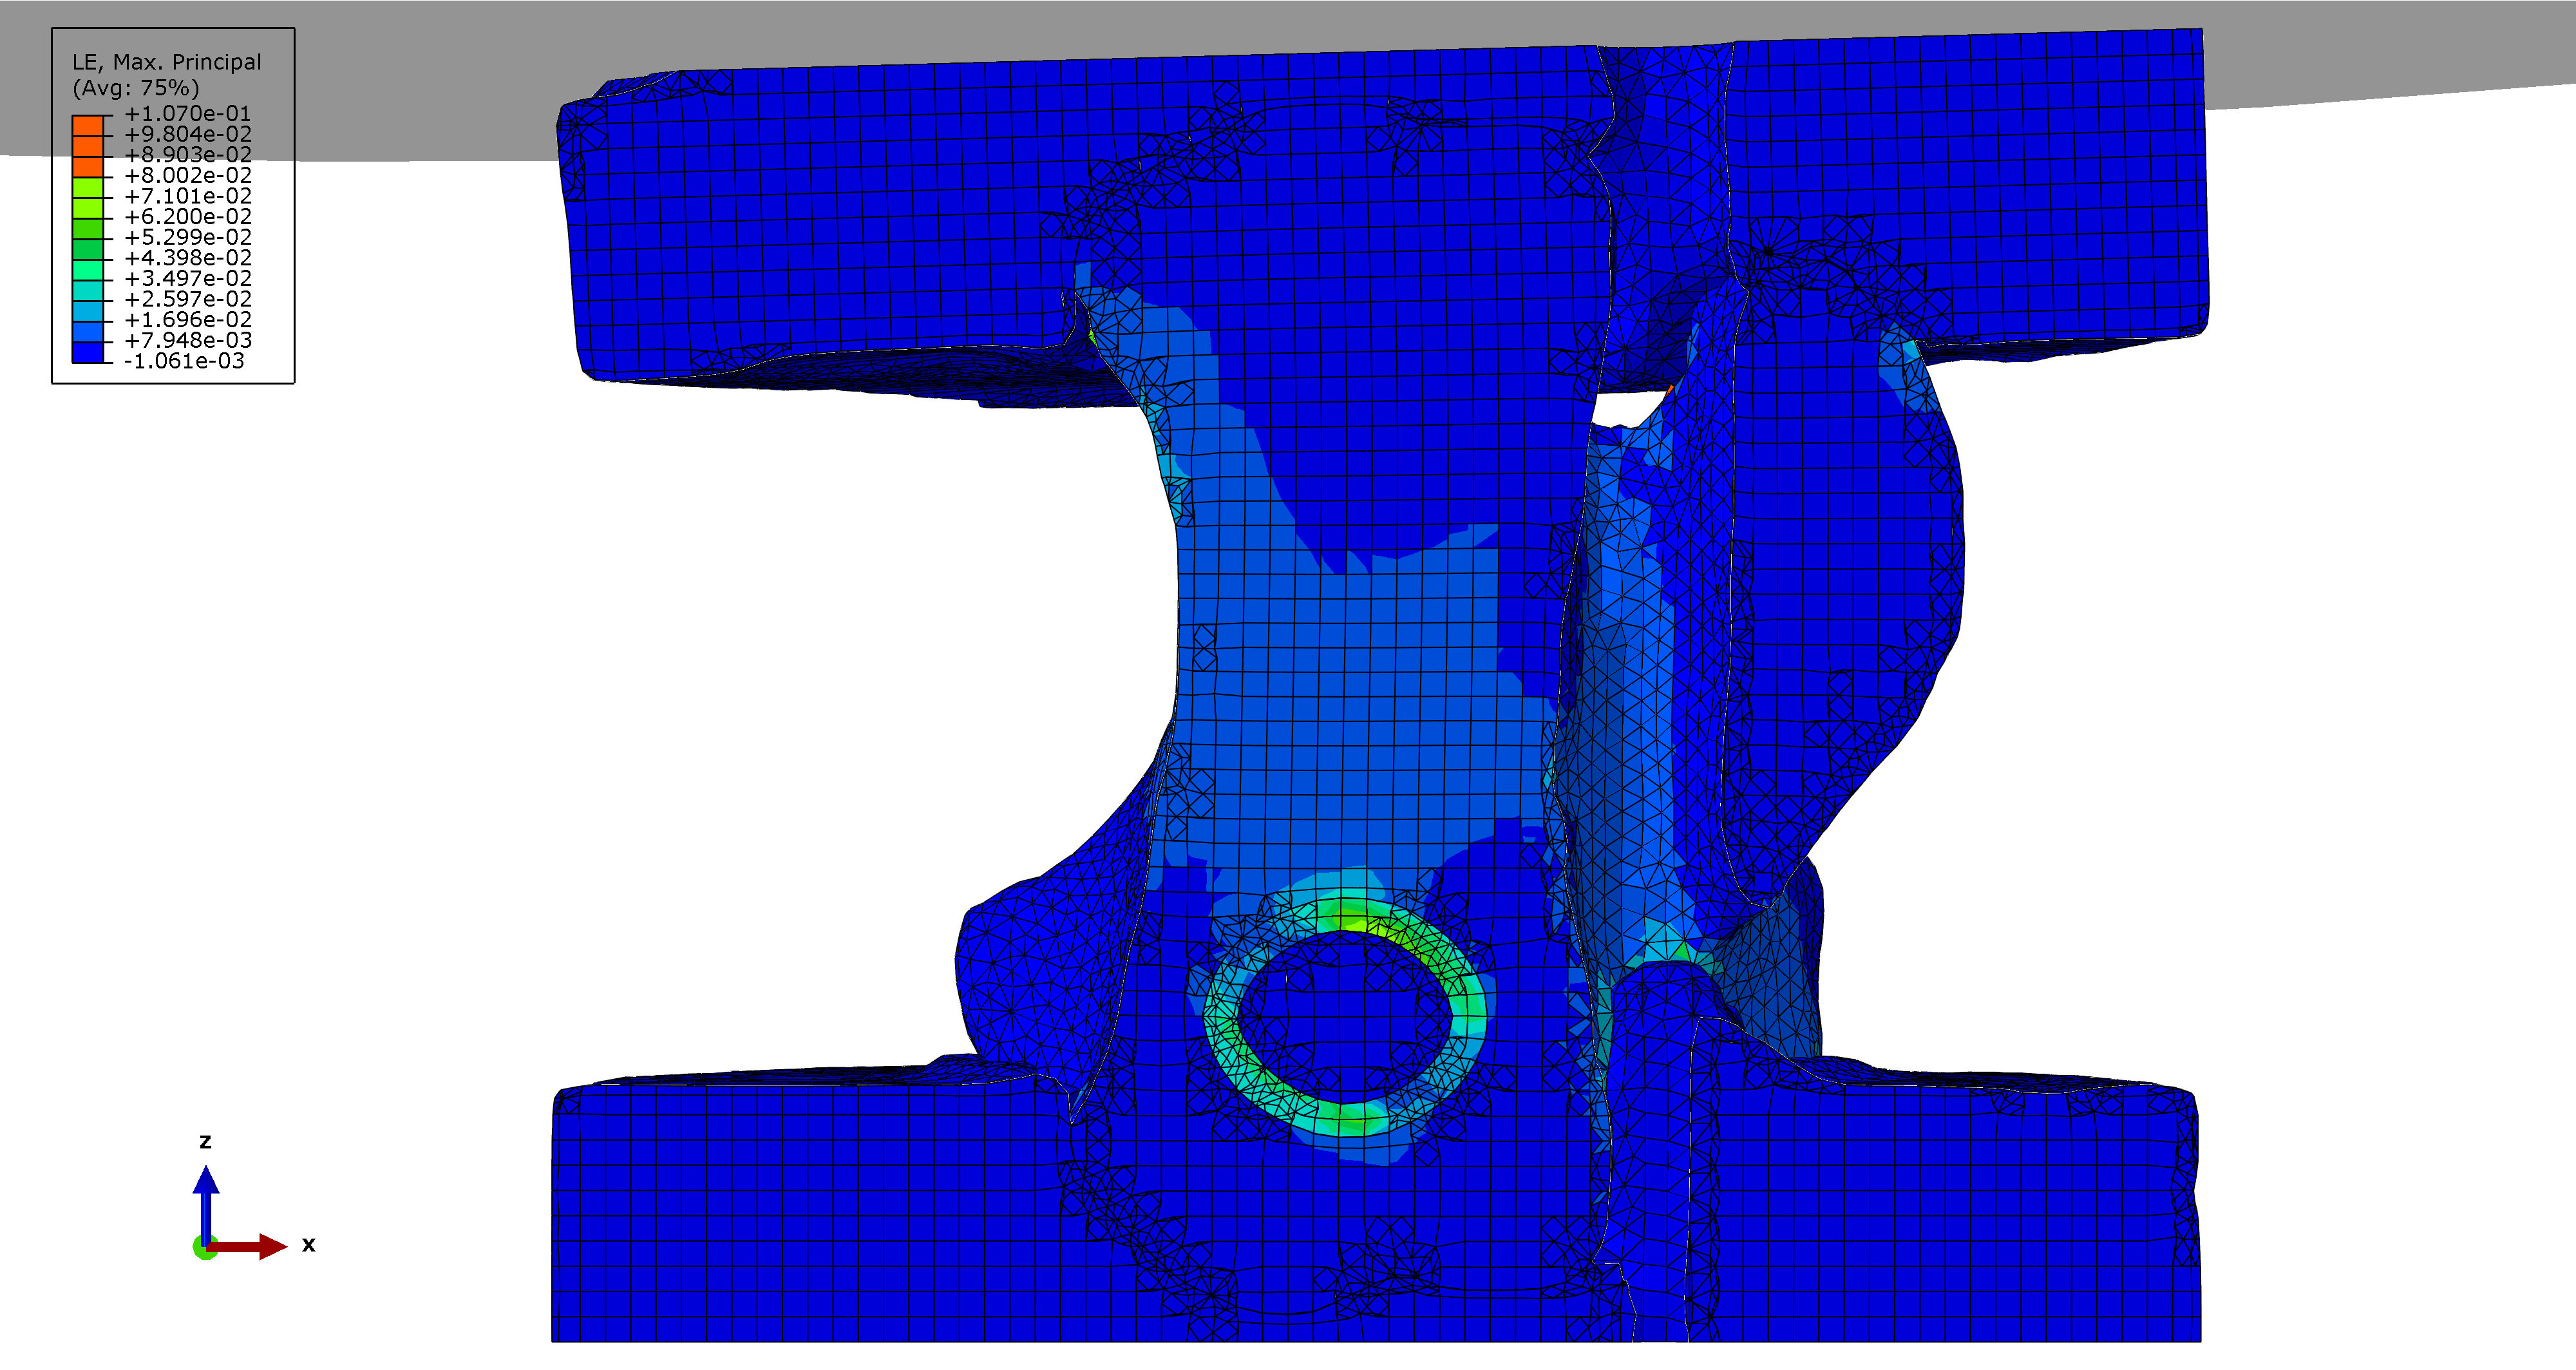
\includegraphics[width=10cm]{images/T2_CC2_intact_MM_cement_Bottom_ABAQUS_Strain.png}   & T2 CC2 \begin{itemize} \item  Computational:	4366  N/mm \item 4 \% Cement Fill \end{itemize} \\ \hline 
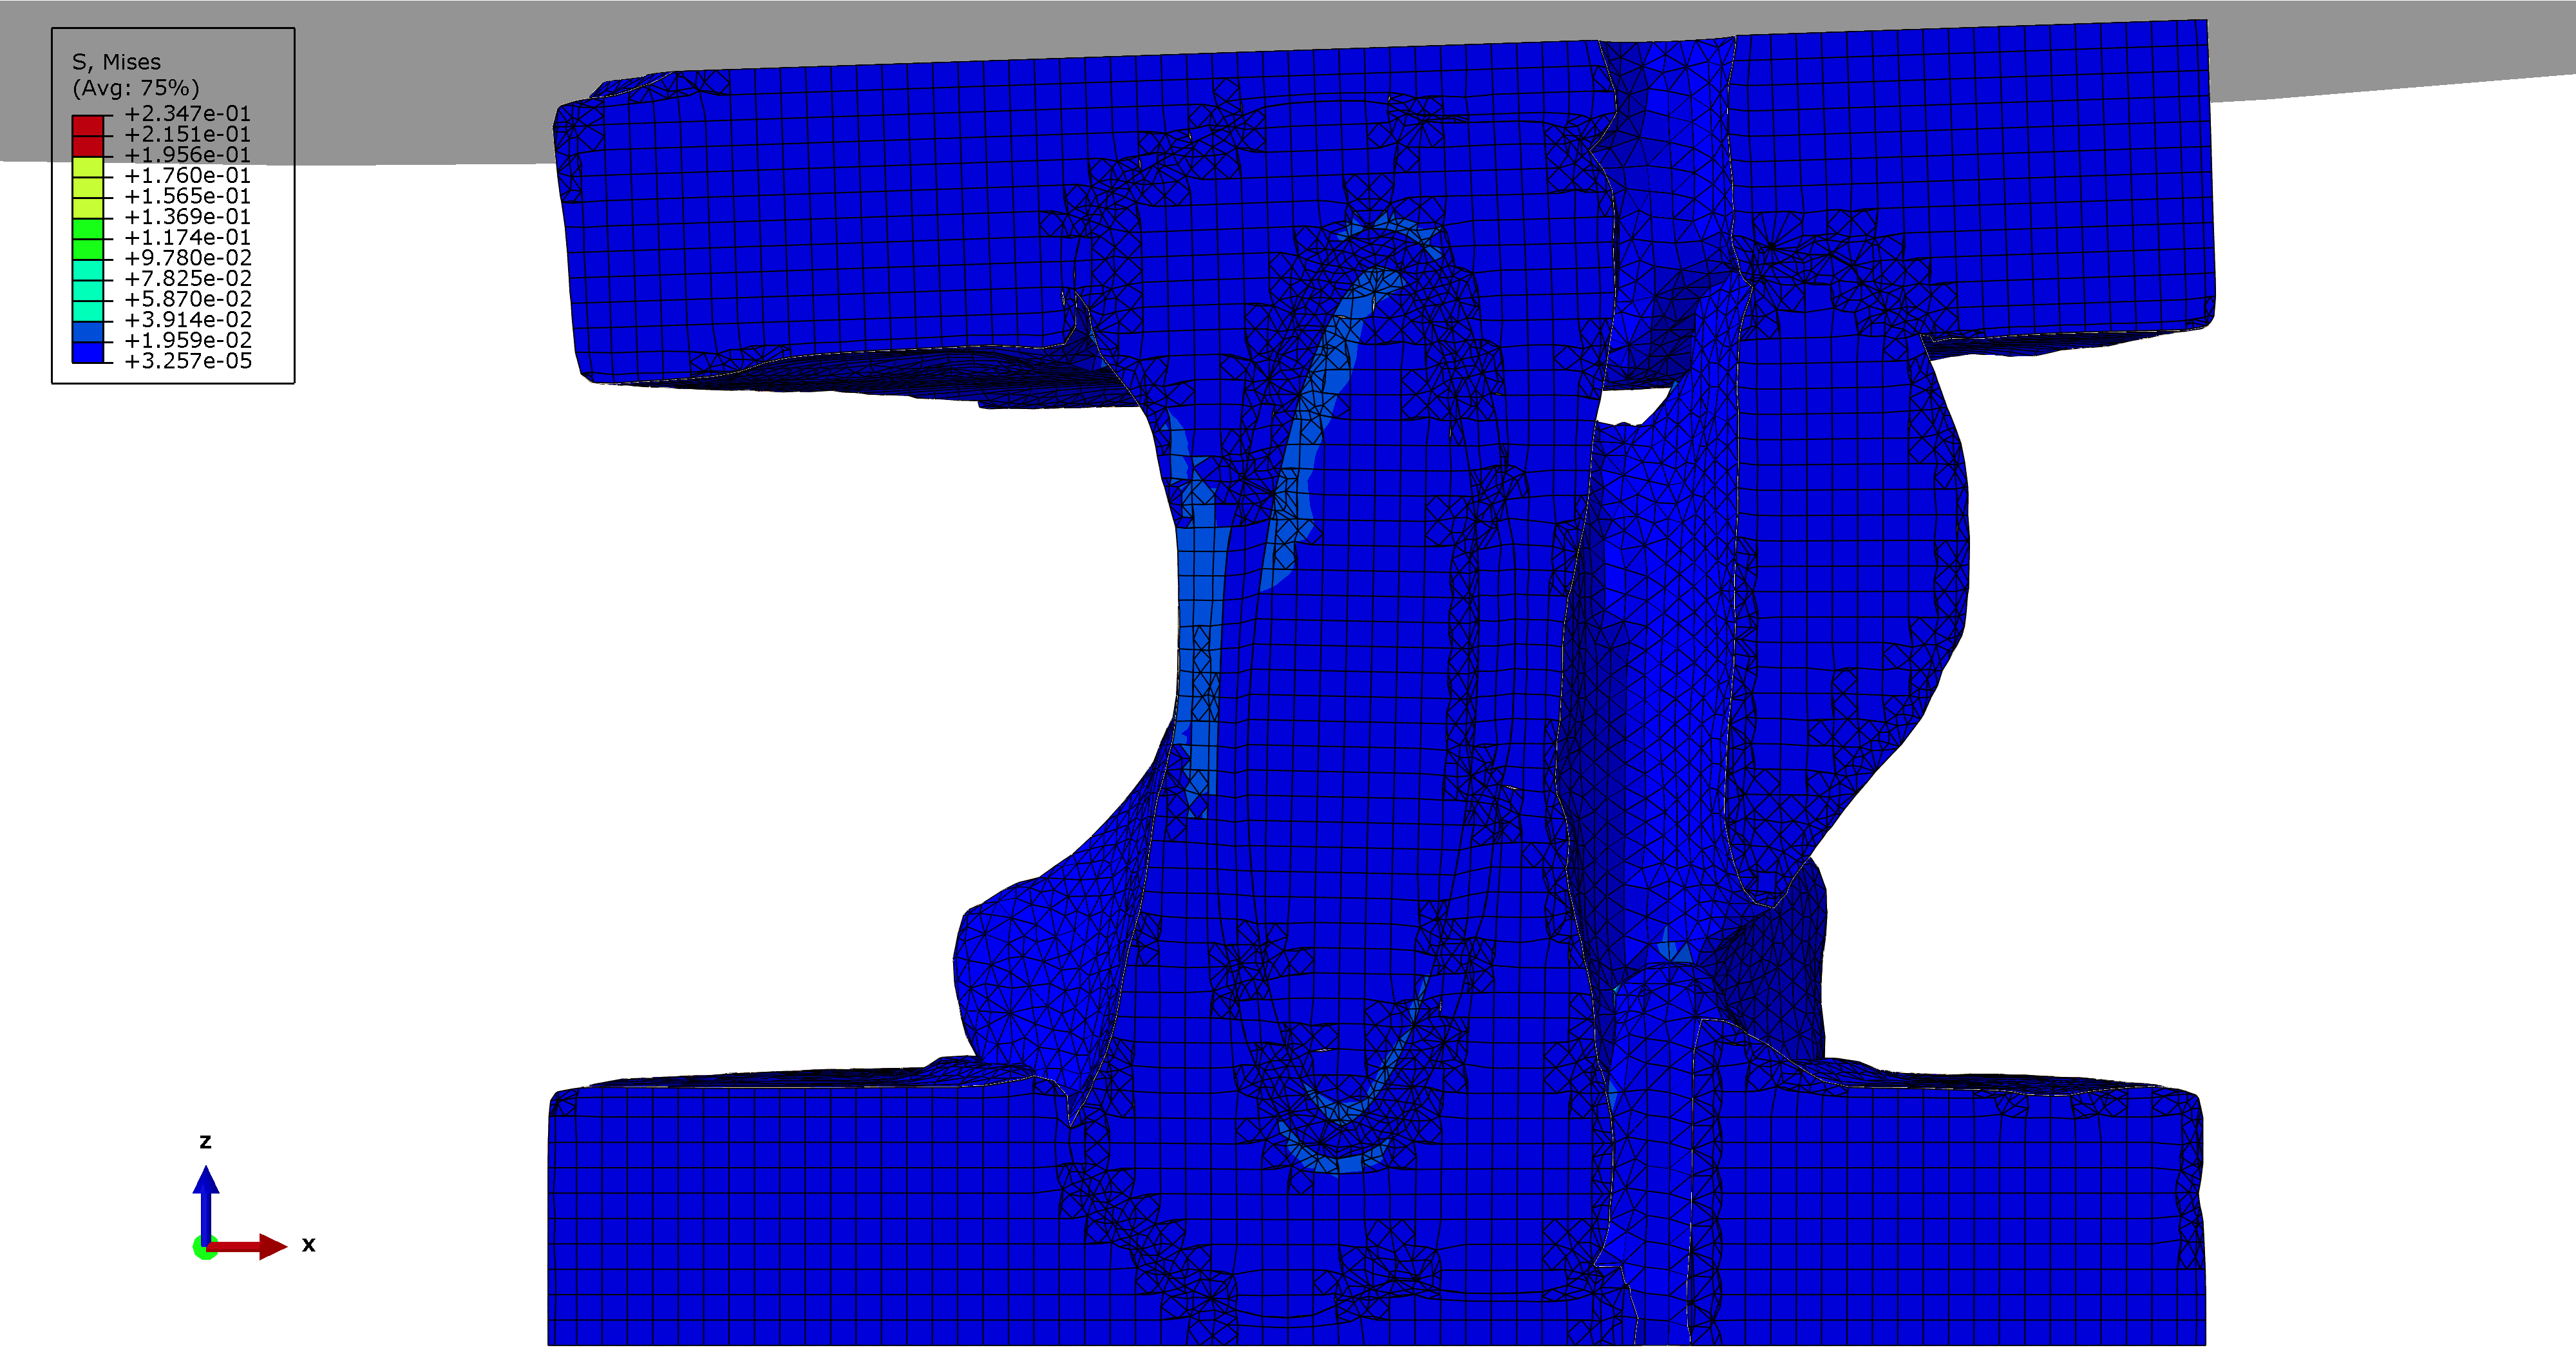
\includegraphics[width=10cm]{images/T2_CC2_intact_MM_cement_Large_Middle_ABAQUS_Stress.png}   & 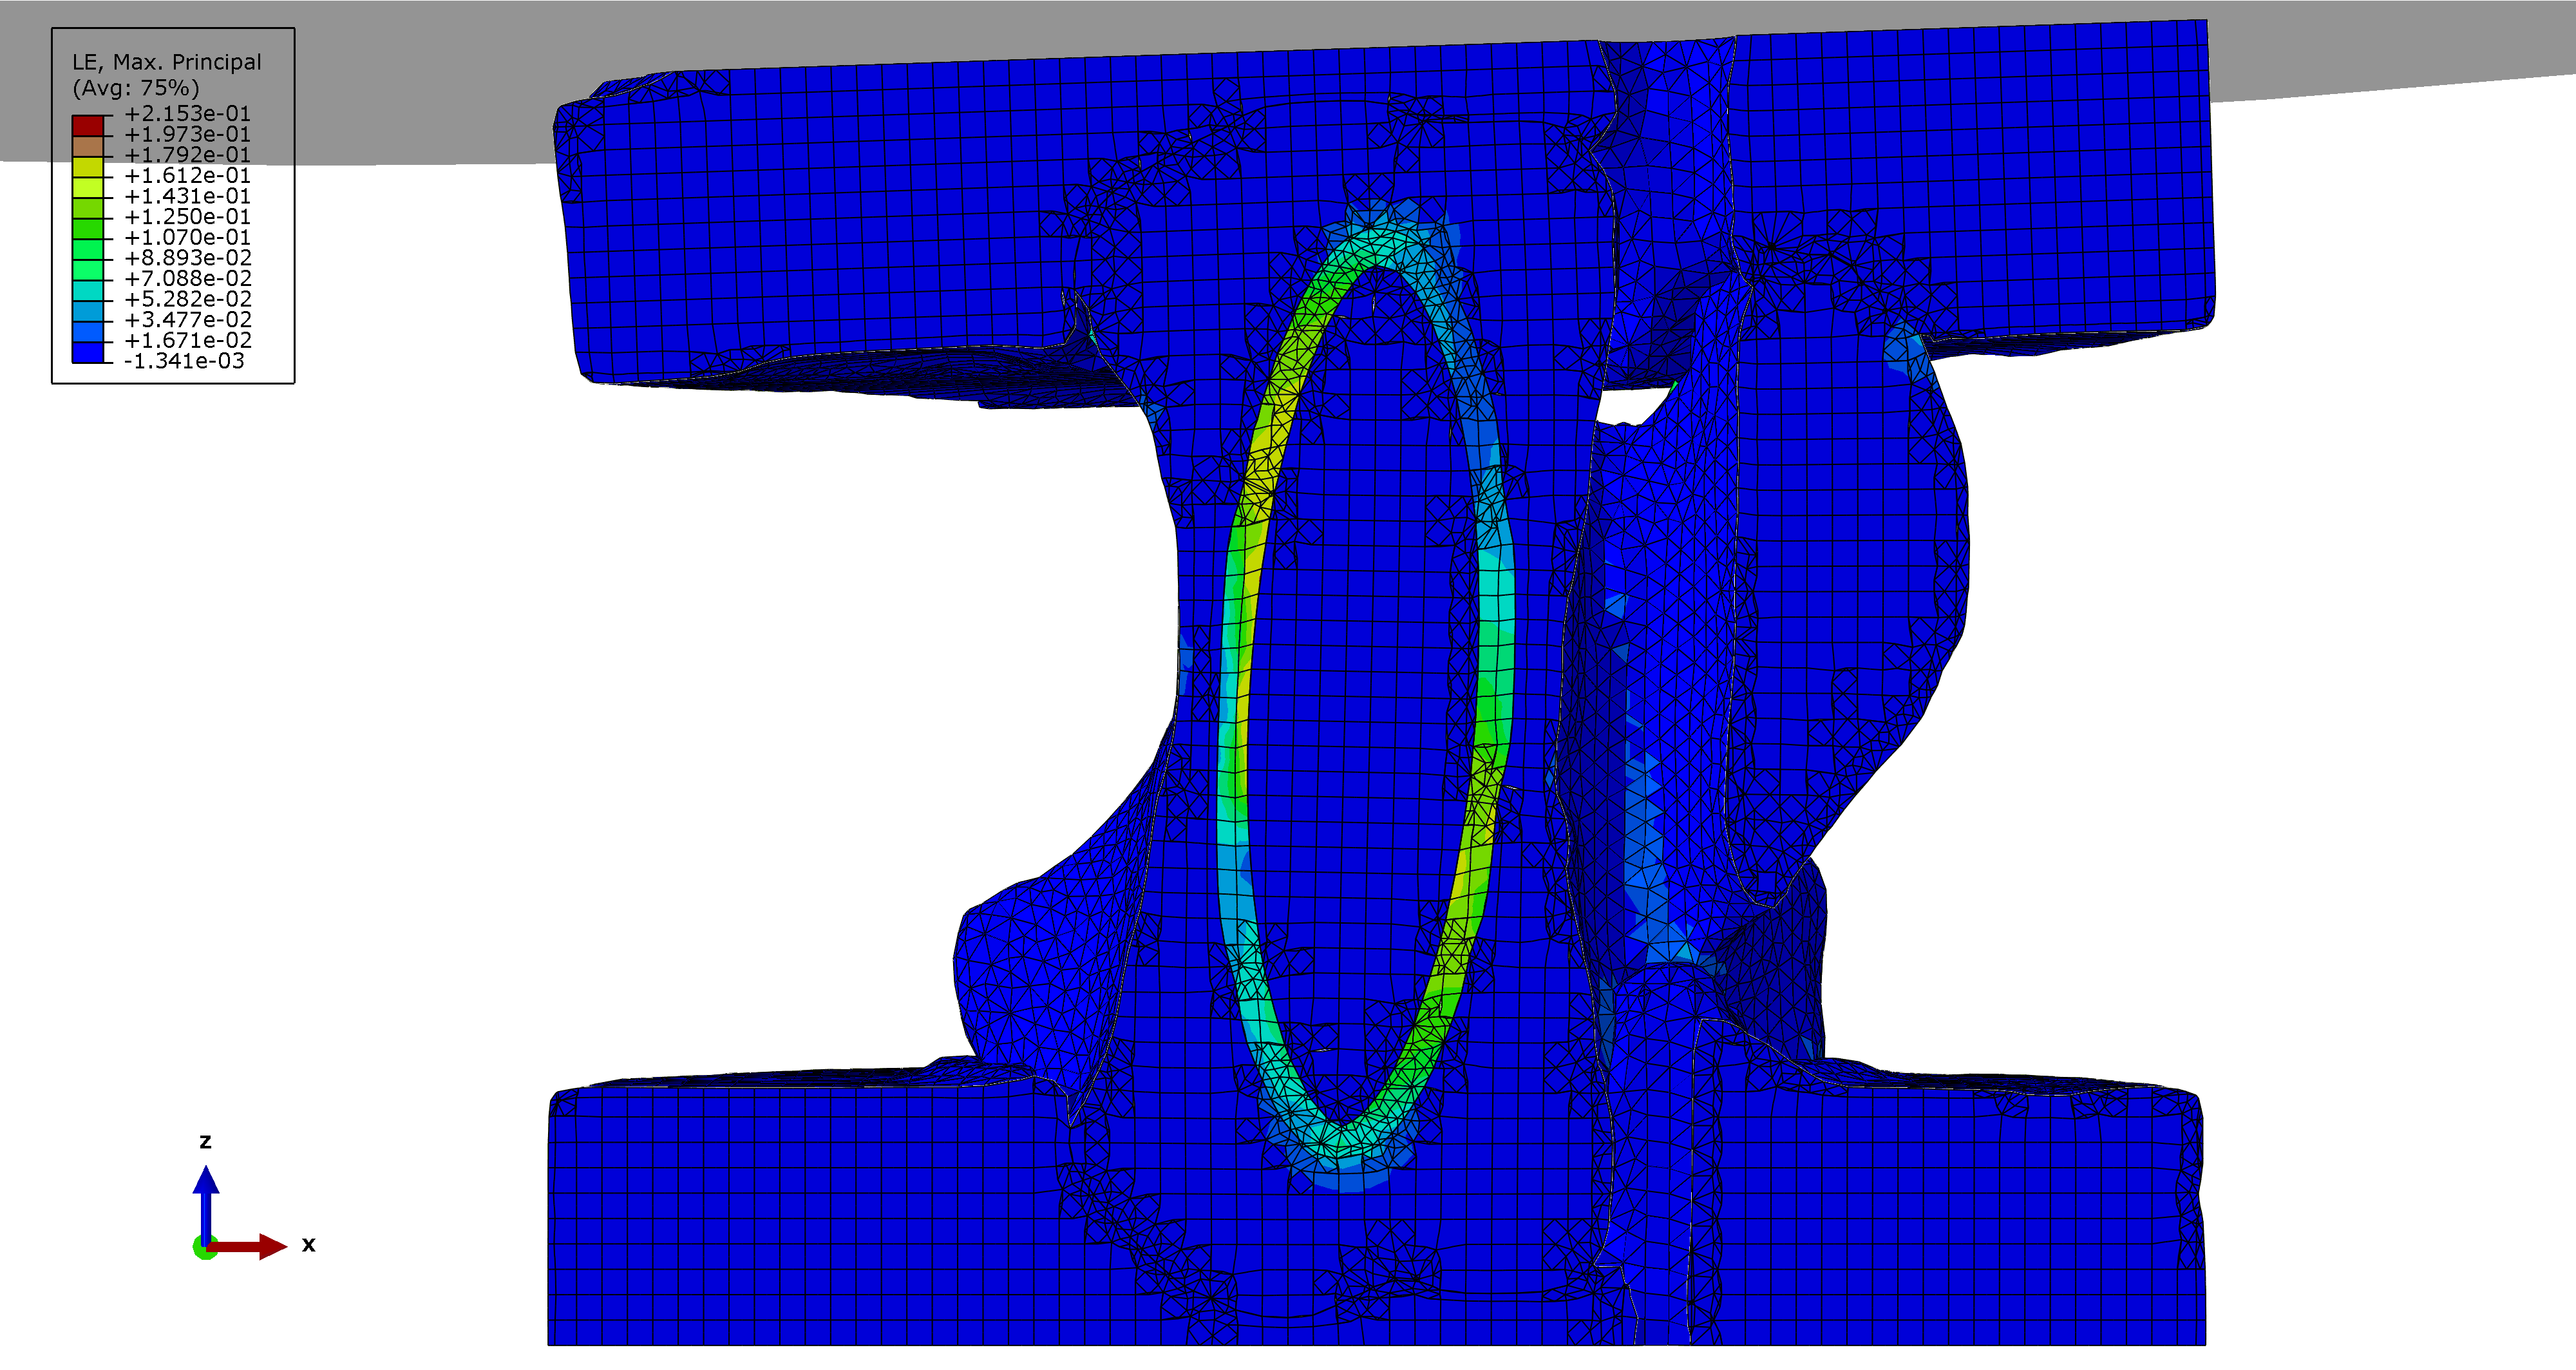
\includegraphics[width=10cm]{images/T2_CC2_intact_MM_cement_Large_Middle_ABAQUS_Strain.png}   & T2 CC2 \begin{itemize} \item  Computational:	2610  N/mm \item 15 \% Cement Fill \end{itemize} \\ \hline 
\end{longtable}

\end{landscape}




\begin{landscape}

\begin{longtable}{|m{11cm}|m{11cm}|m{4cm}|}
Stress & Strain & Details \\ \hline
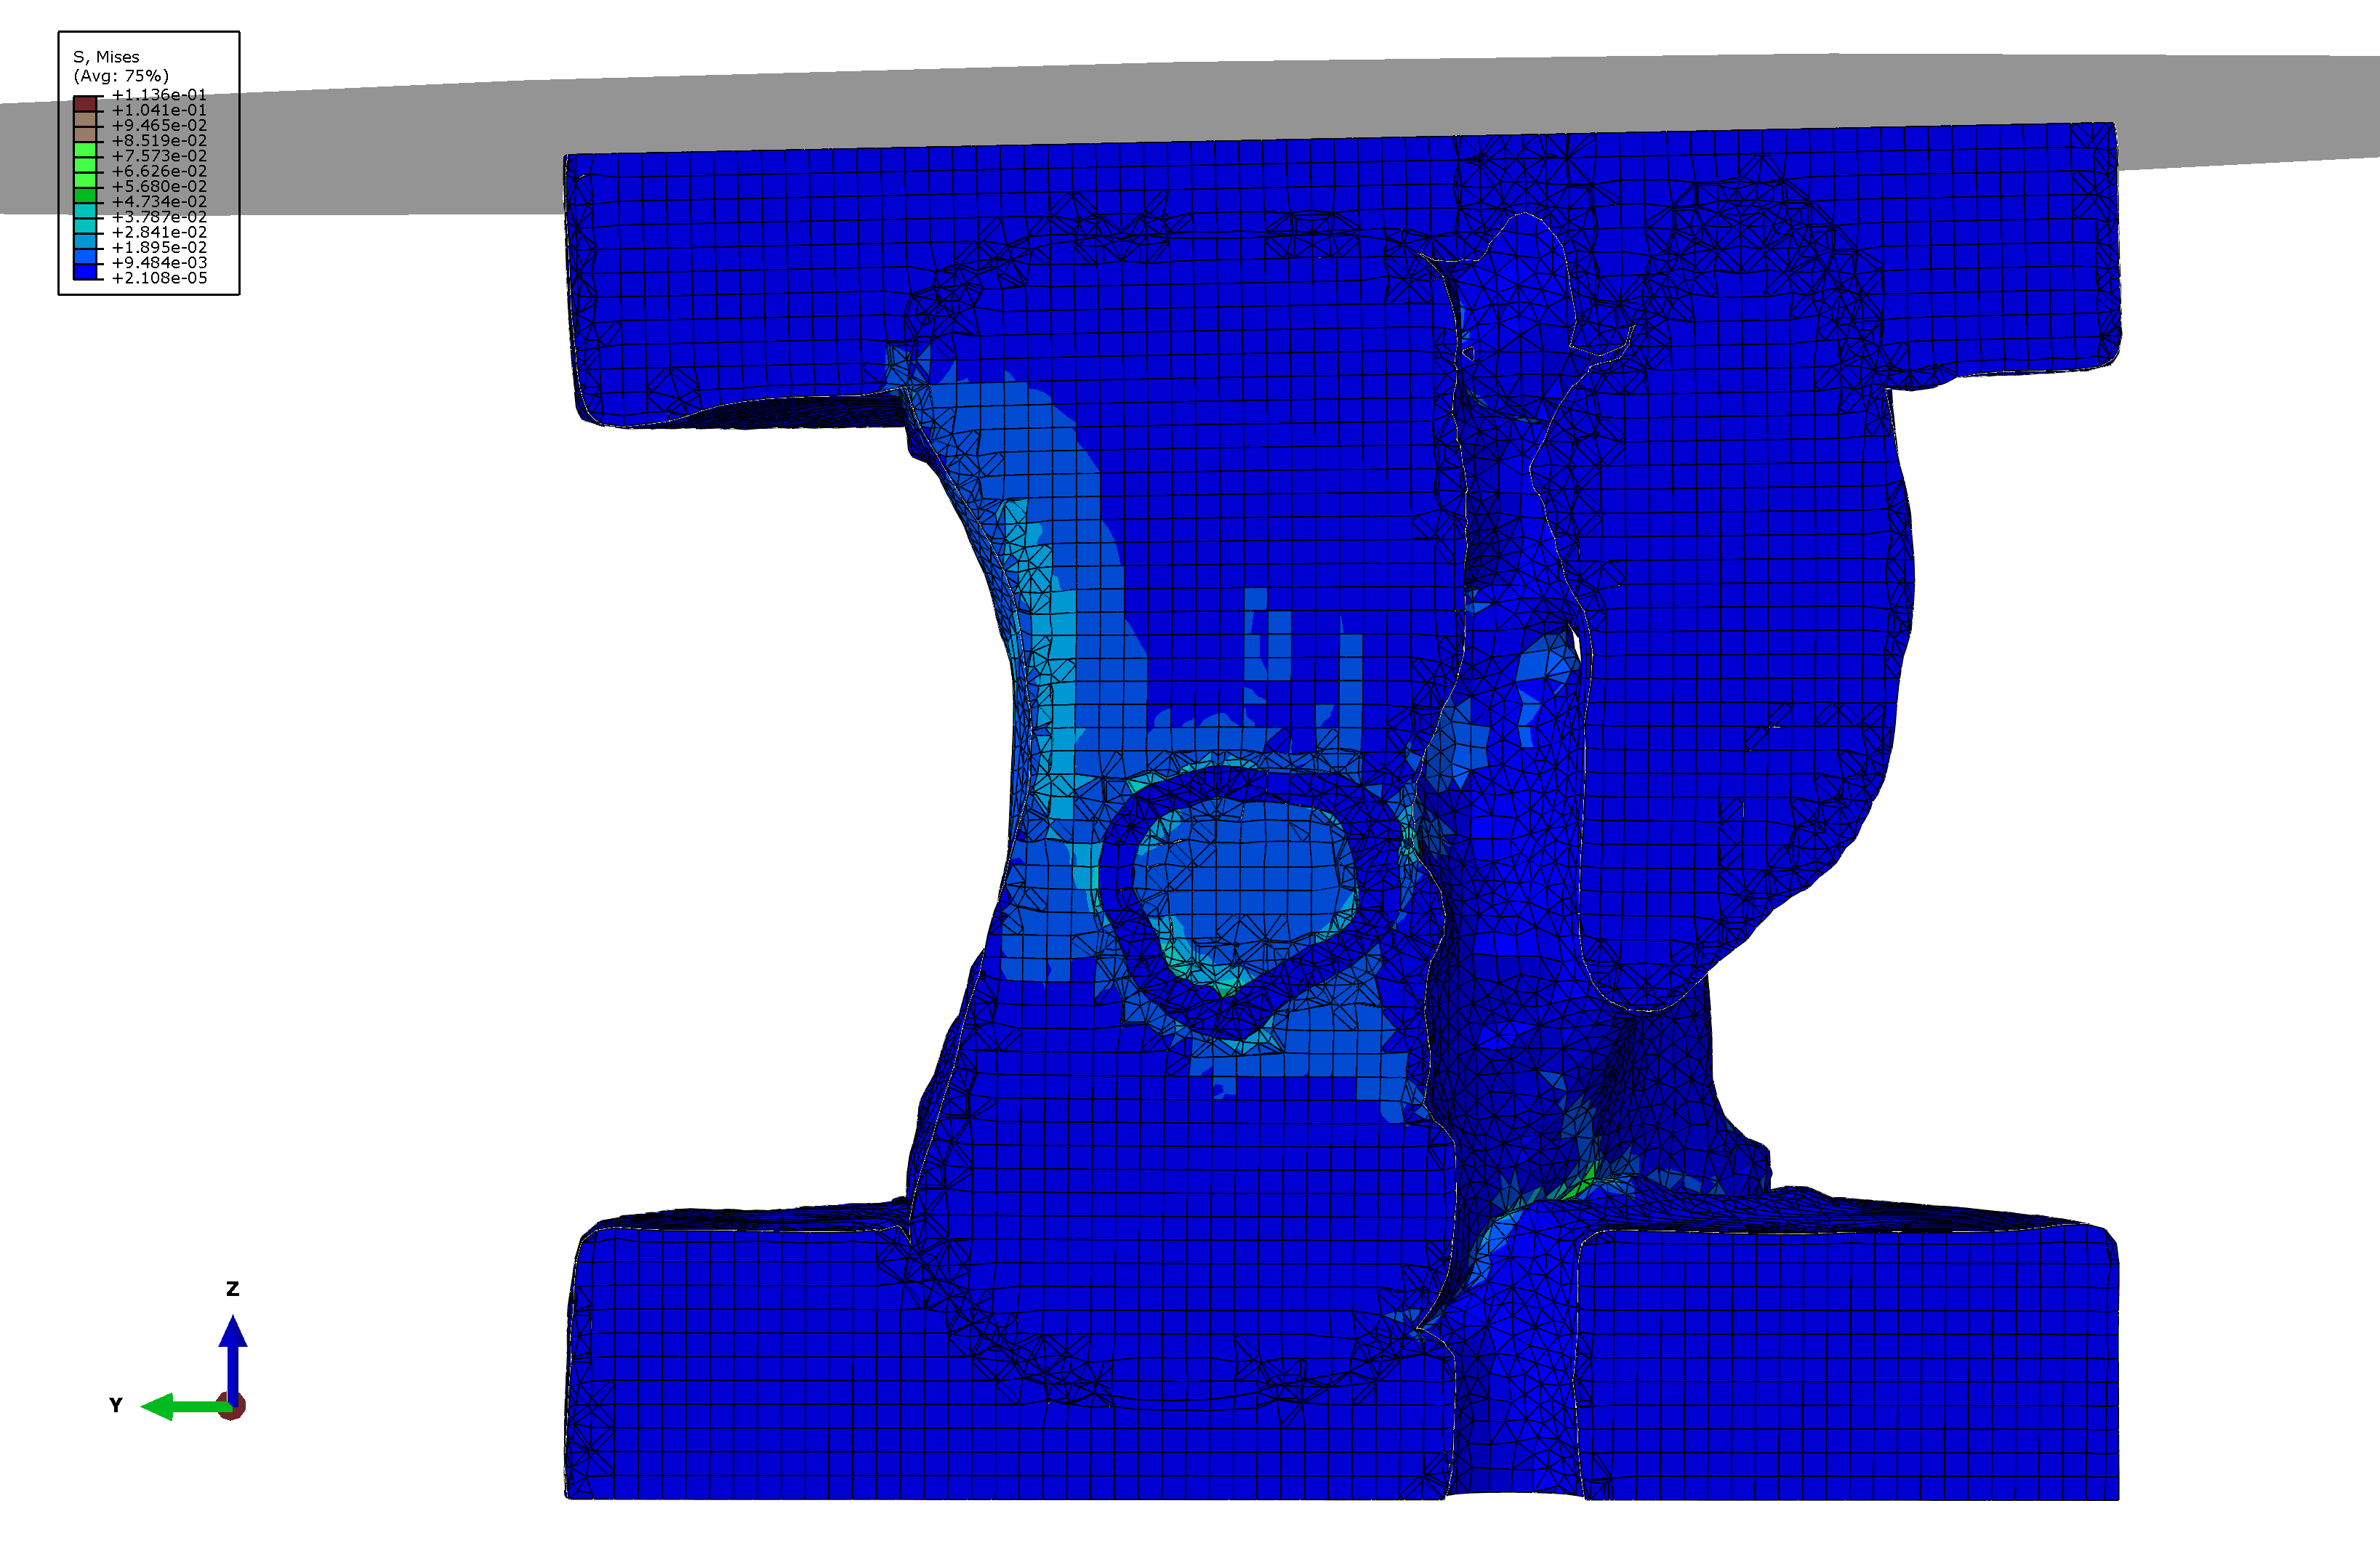
\includegraphics[width=10cm]{images/T1_CC1_postVP_Interface_ABAQUS_All_Side_Stress.png}   & 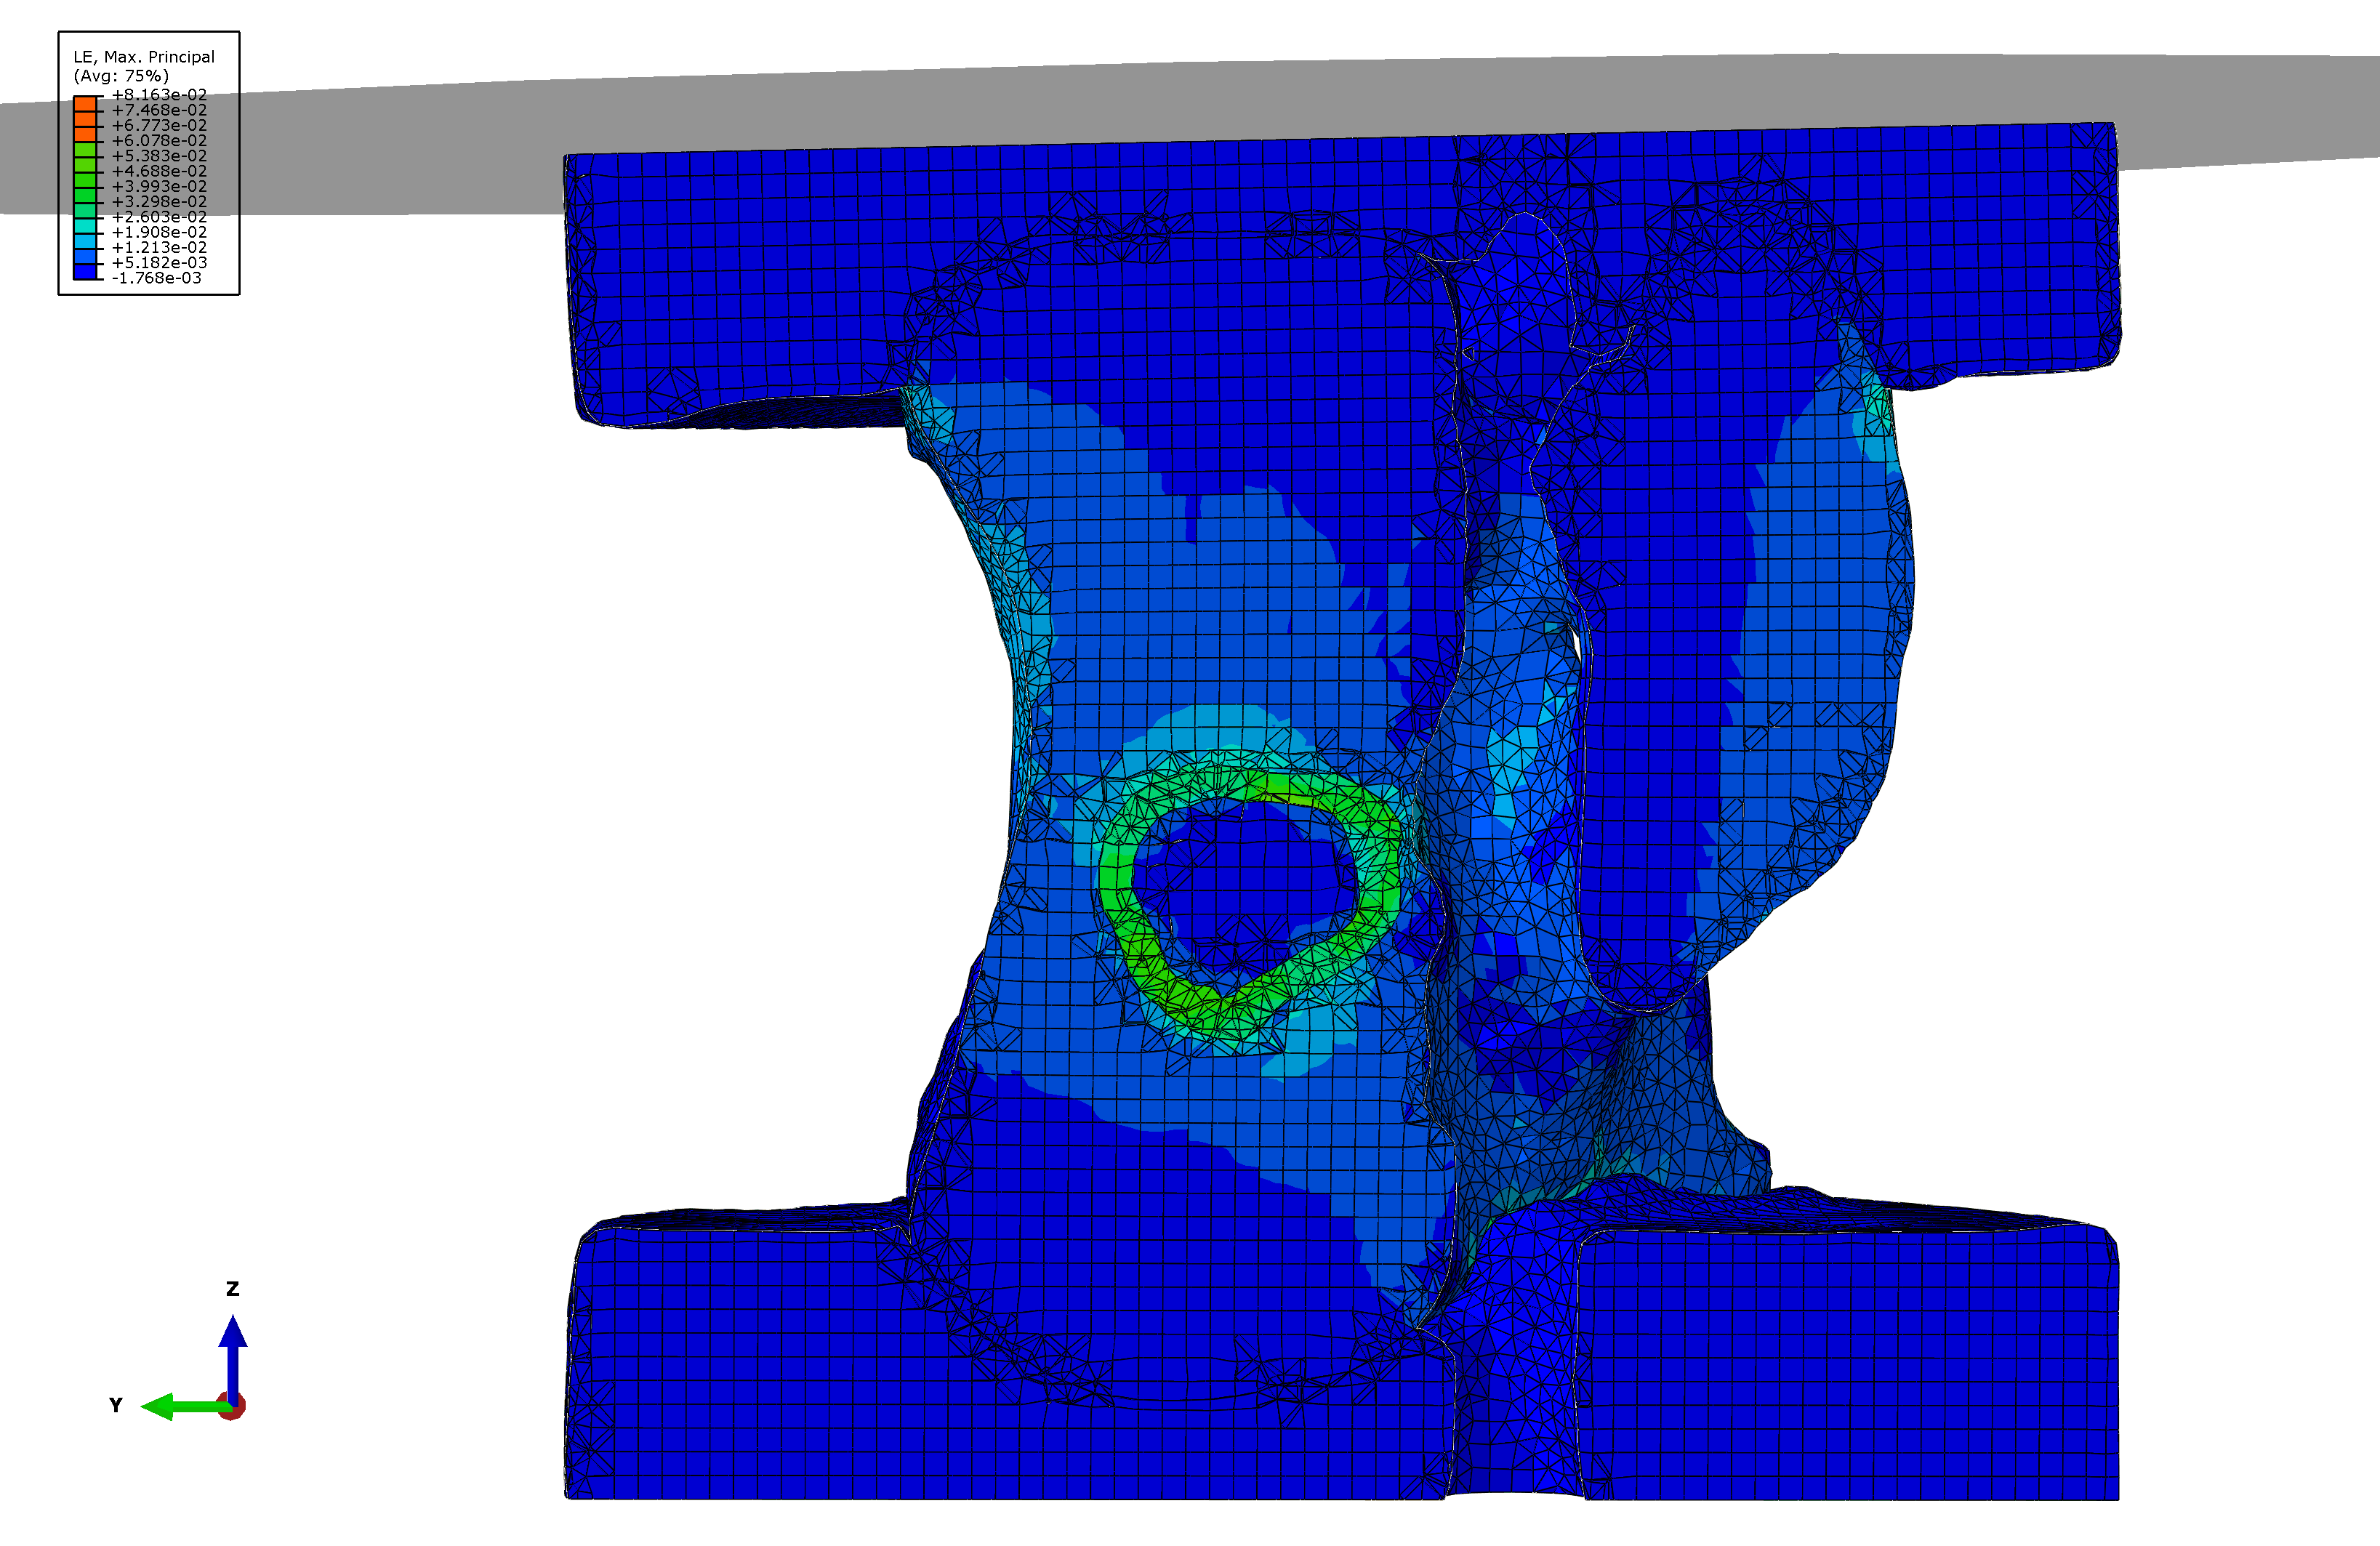
\includegraphics[width=10cm]{images/T1_CC1_postVP_Interface_ABAQUS_All_Side_Strain.png}   & T1 CC1 \begin{itemize} \item Experimental: 	4617.3	N/mm  \item Computational:	4703.5  N/mm \item 6.5 \% Fill \end{itemize} \\ \hline 

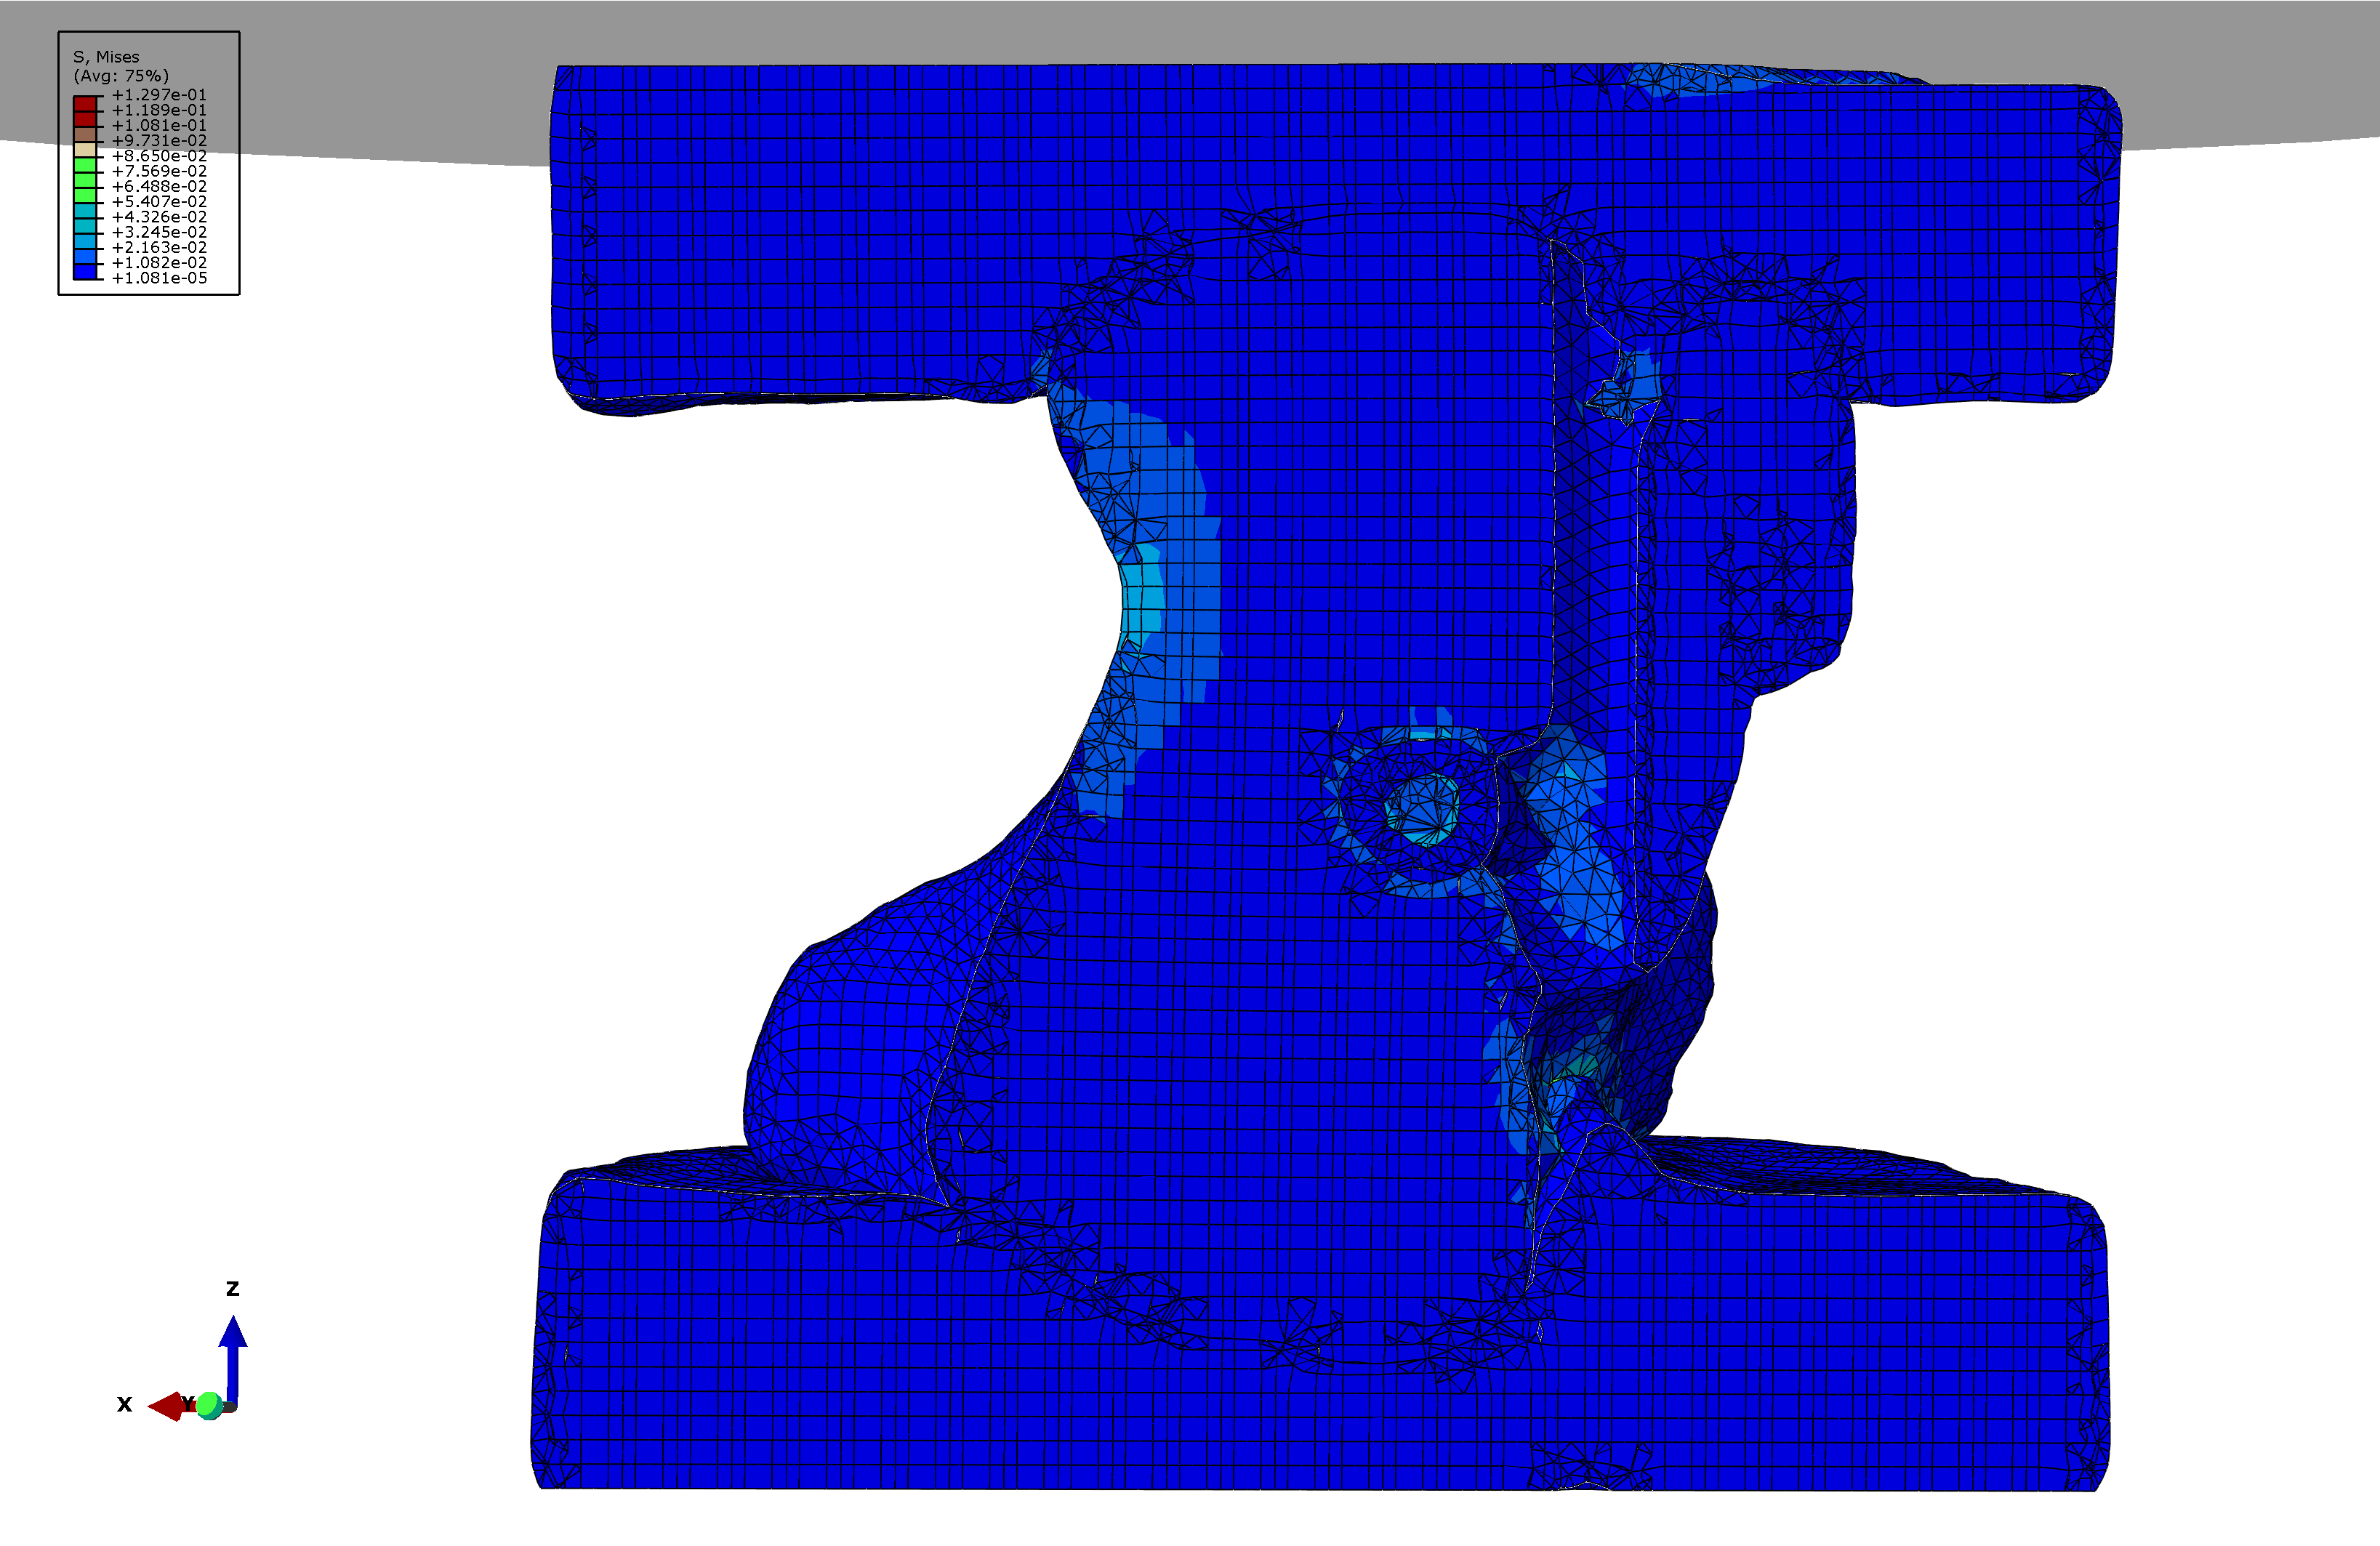
\includegraphics[width=10cm]{images/T1_CC3_postVP_Interface_ABAQUS_All_Side_Stress.png}   & 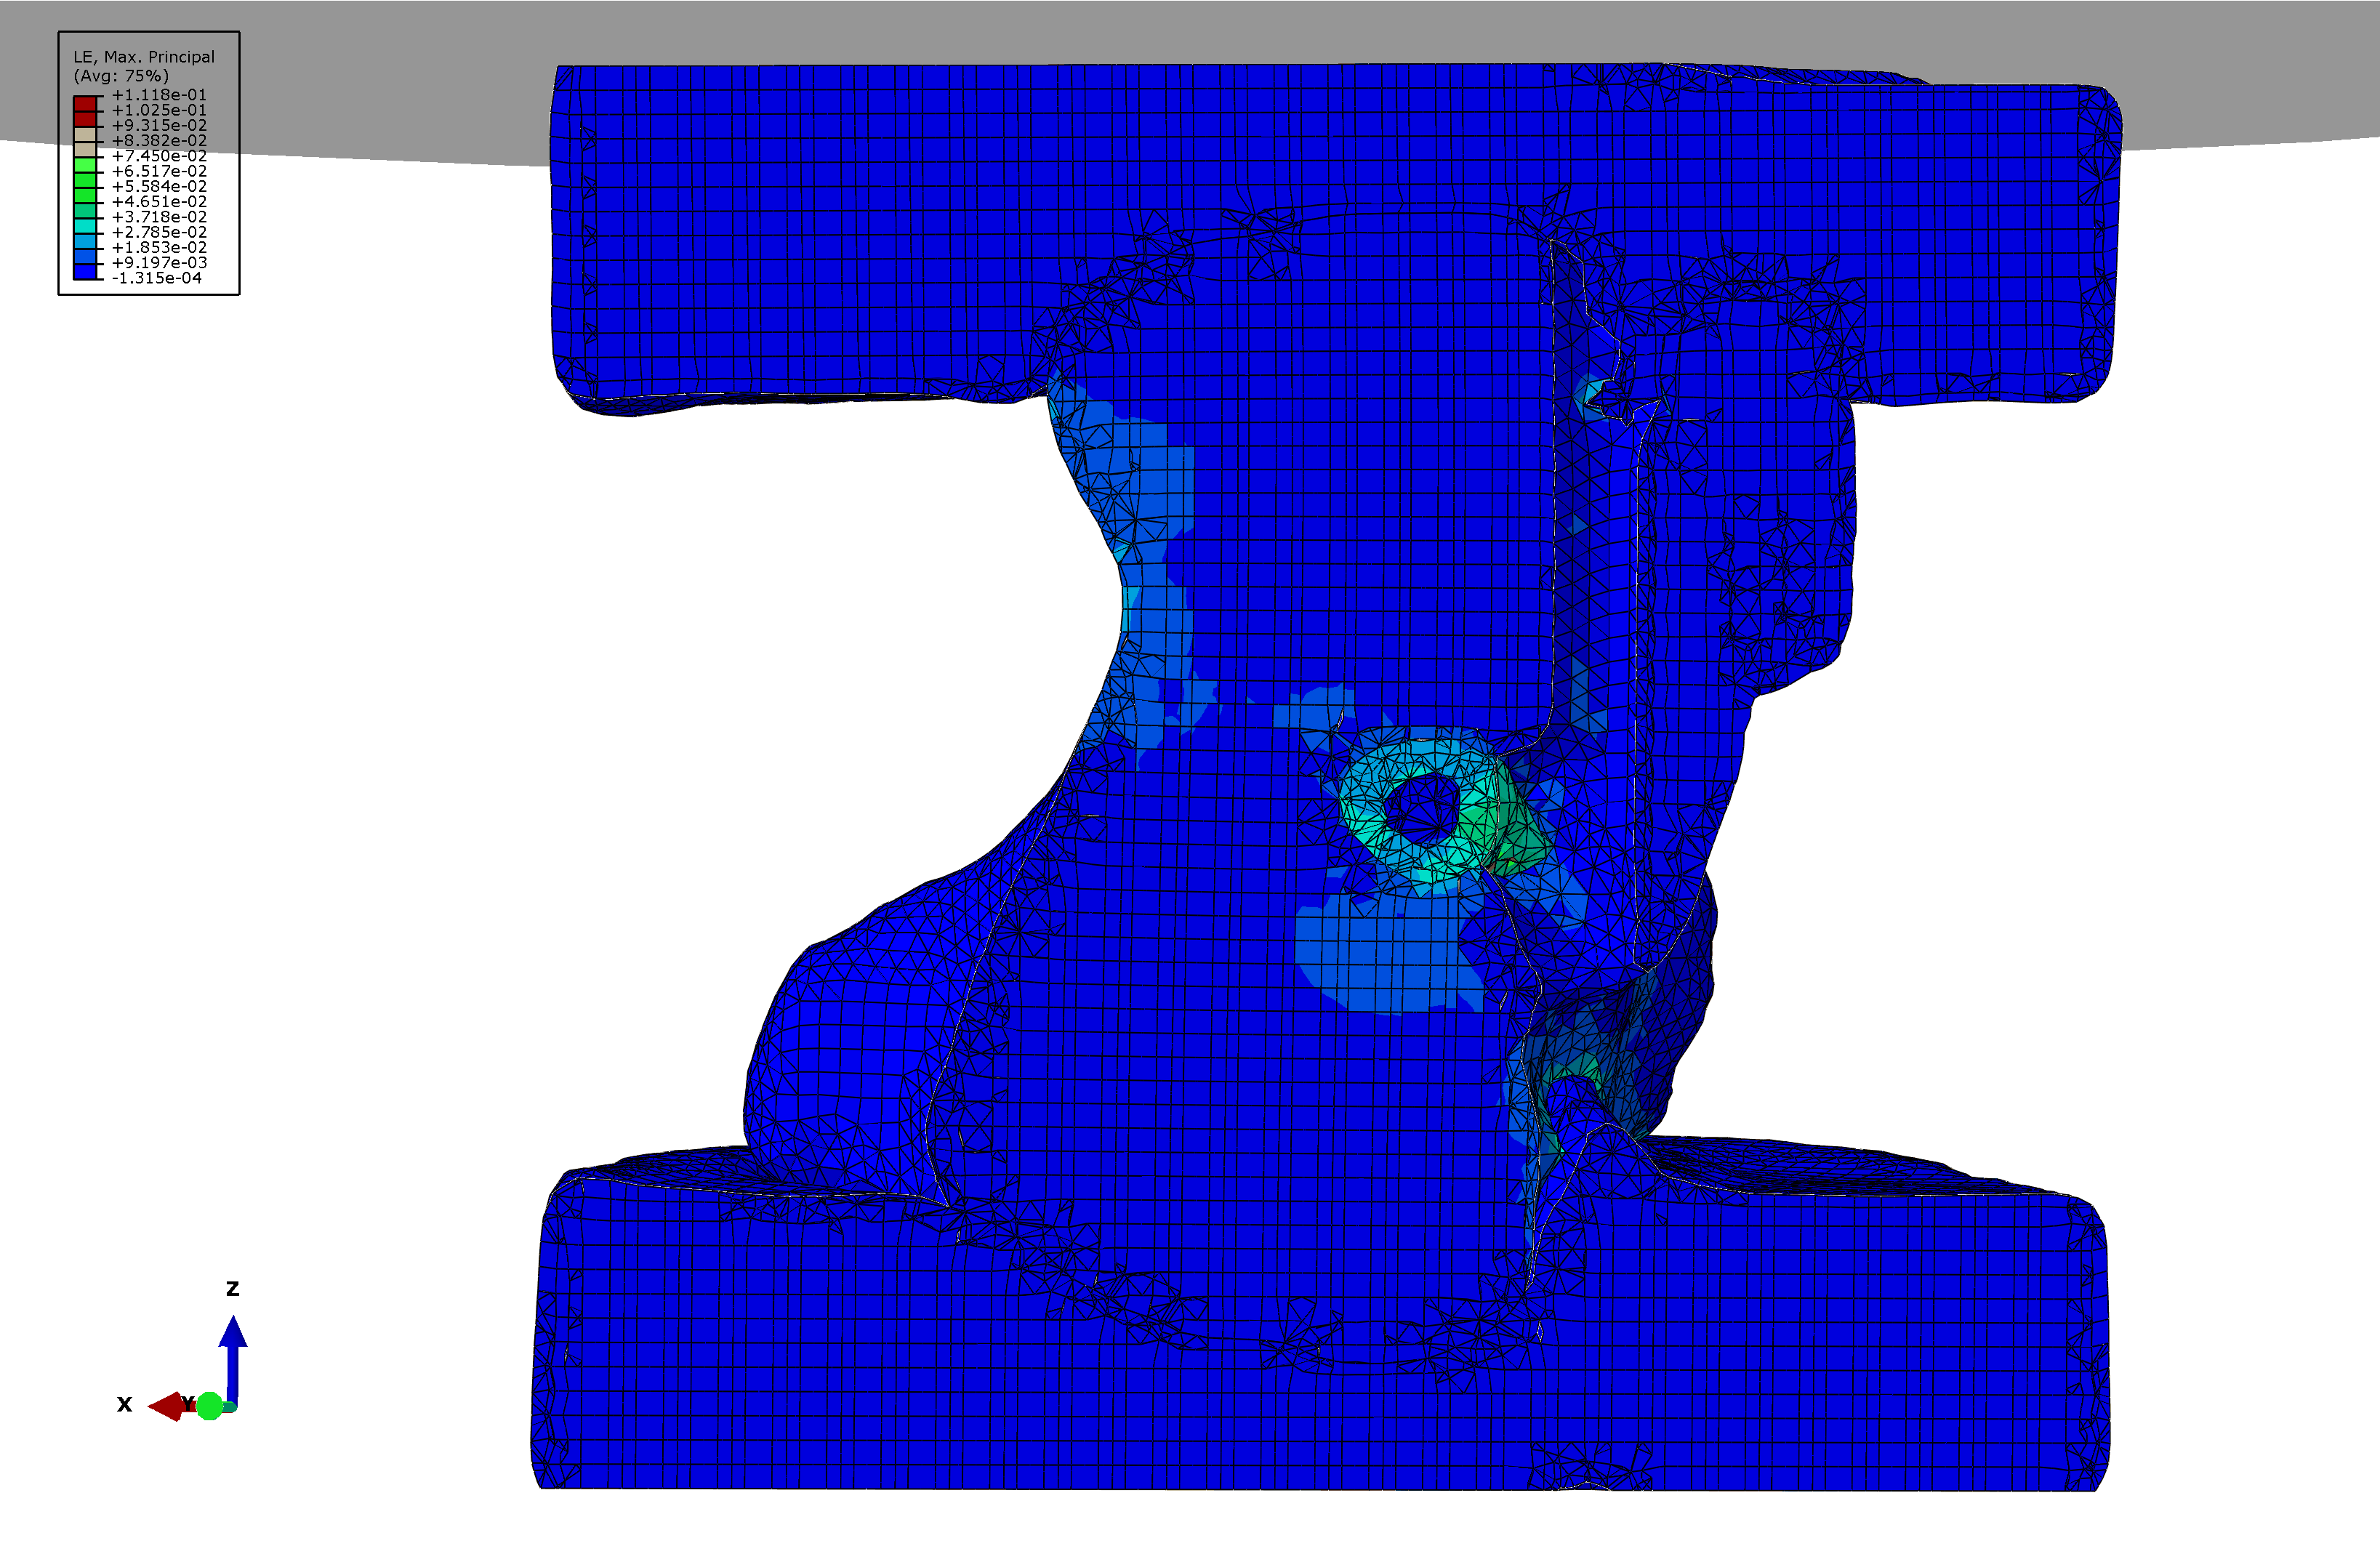
\includegraphics[width=10cm]{images/T1_CC3_postVP_Interface_ABAQUS_All_Side_Strain.png}   & T1 CC3  \begin{itemize} \item Experimental: 	4883.3	N/mm \item Computational:	3677.75 N/mm \item 1.7 \% Fill \end{itemize} \\ \hline 
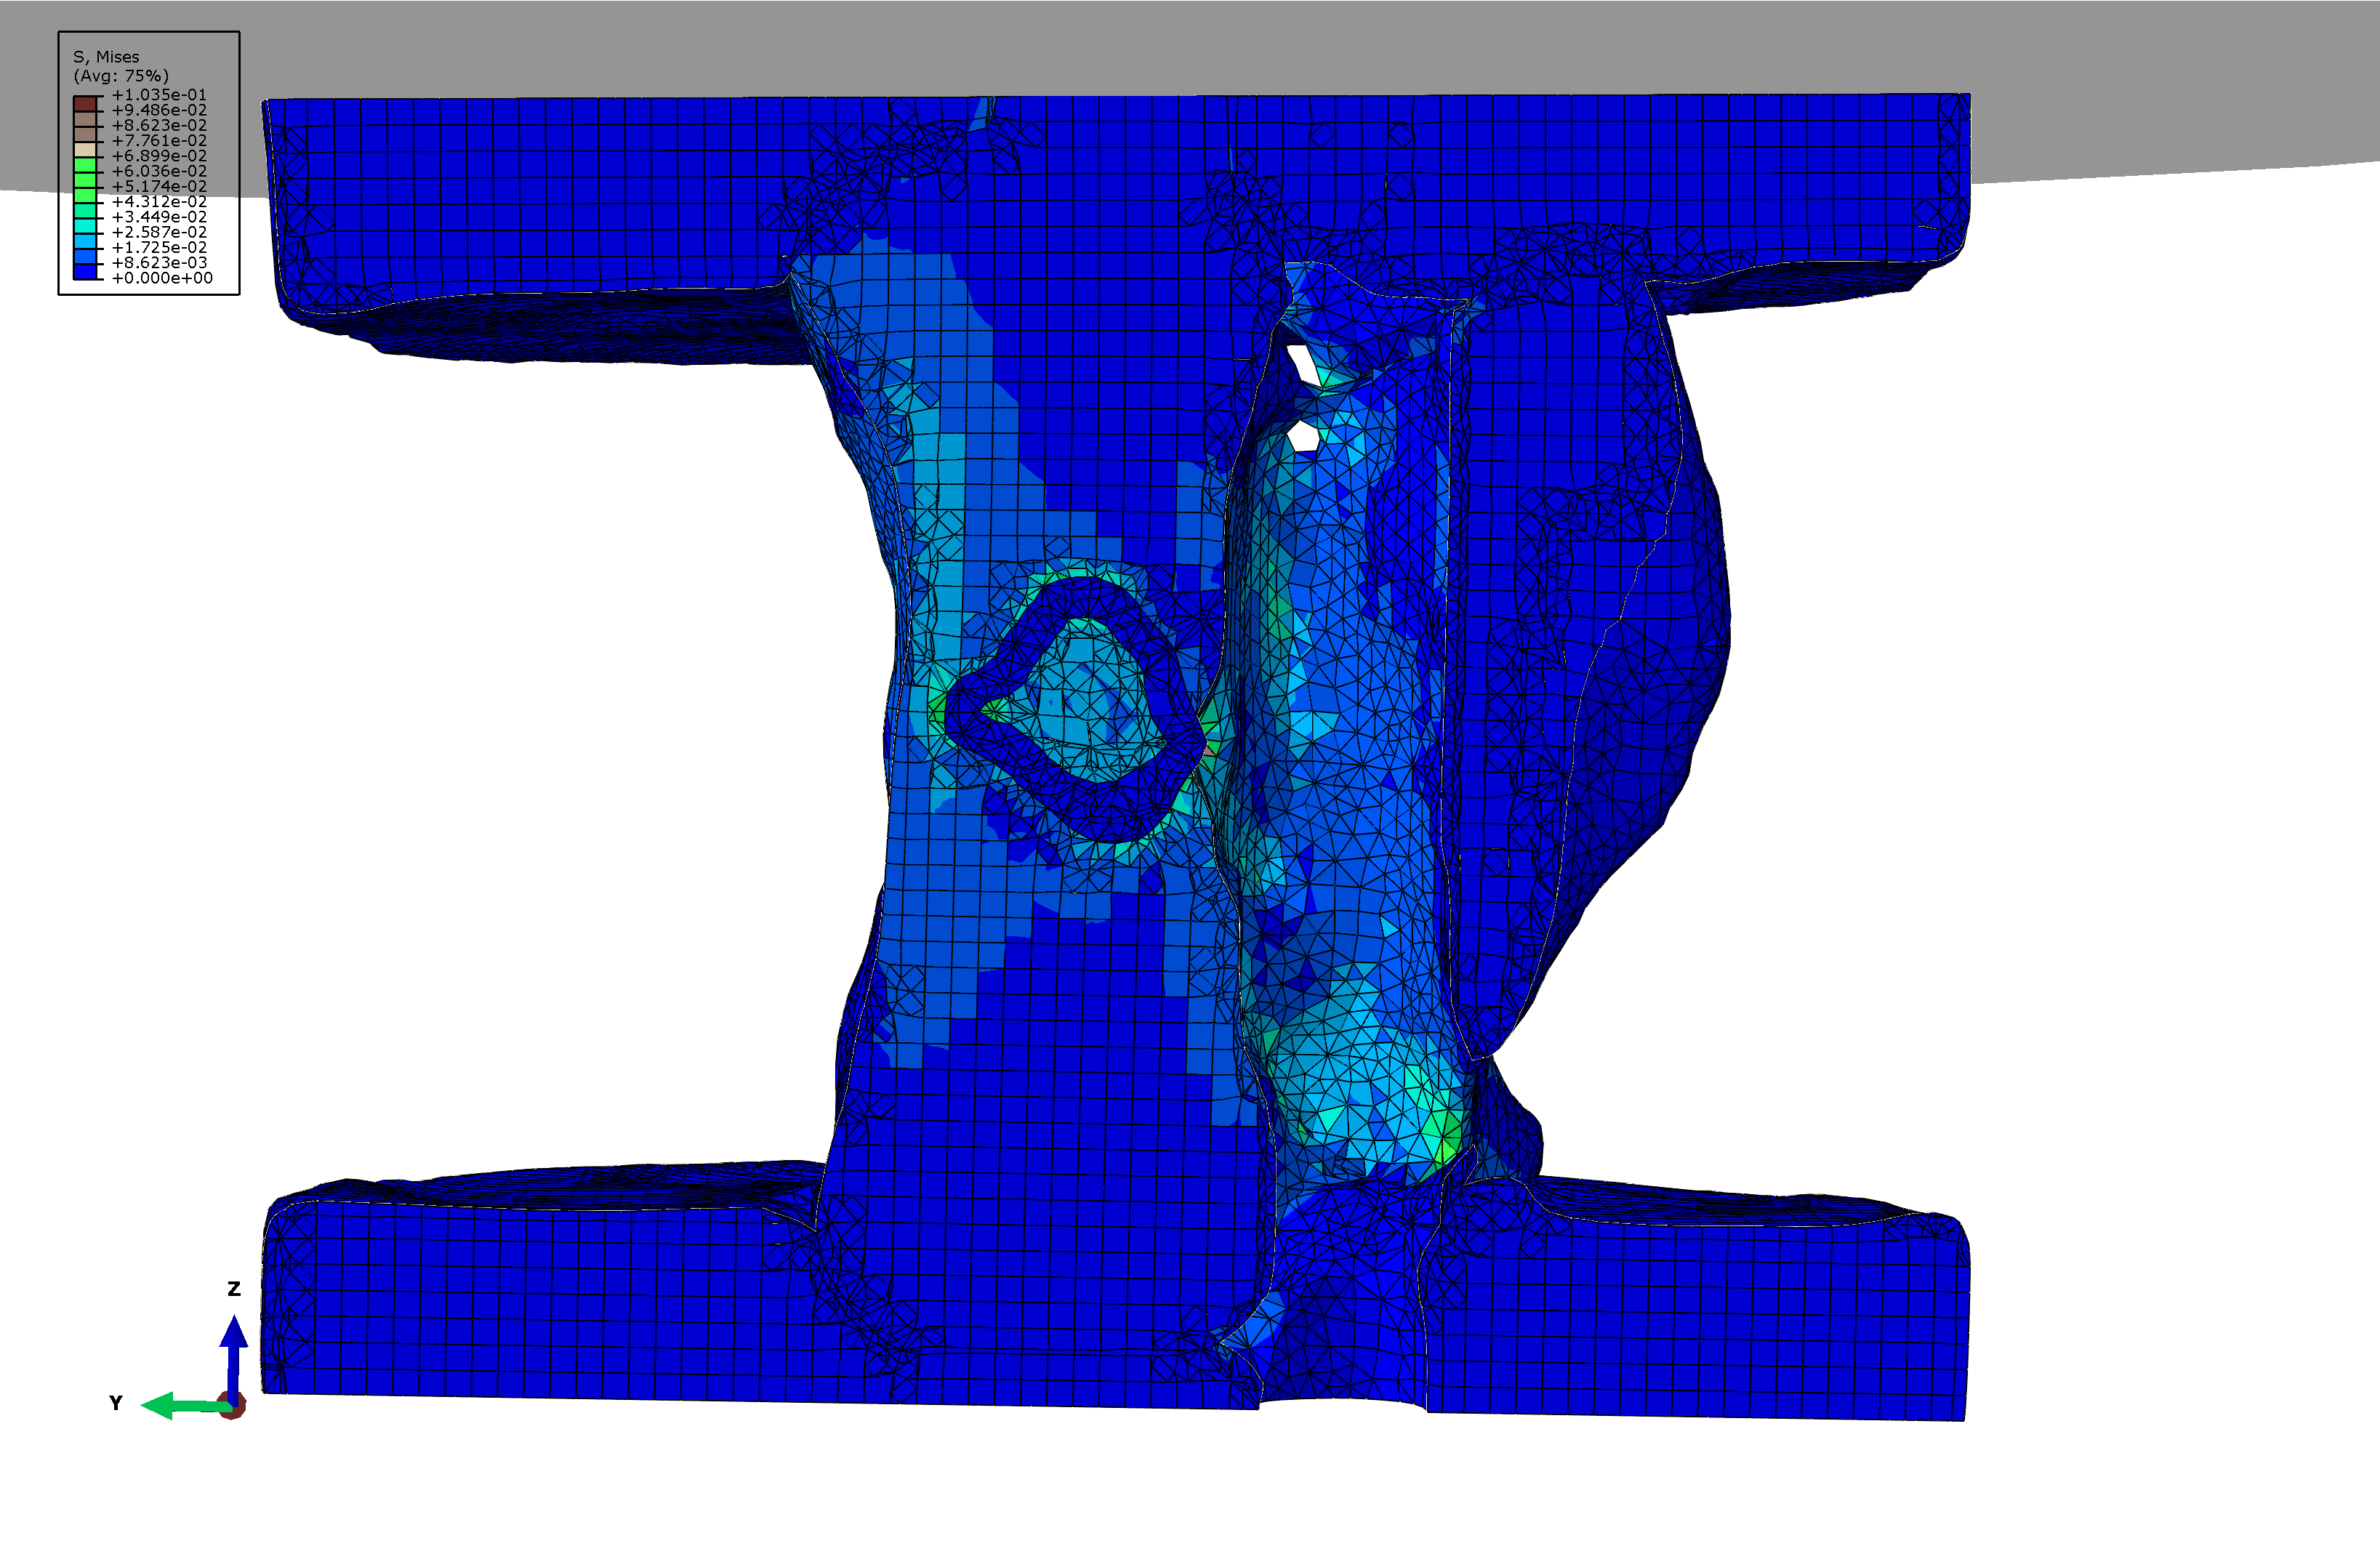
\includegraphics[width=10cm]{images/T2_CC1_postVP_Interface_ABAQUS_All_Side_Stress.png}   & 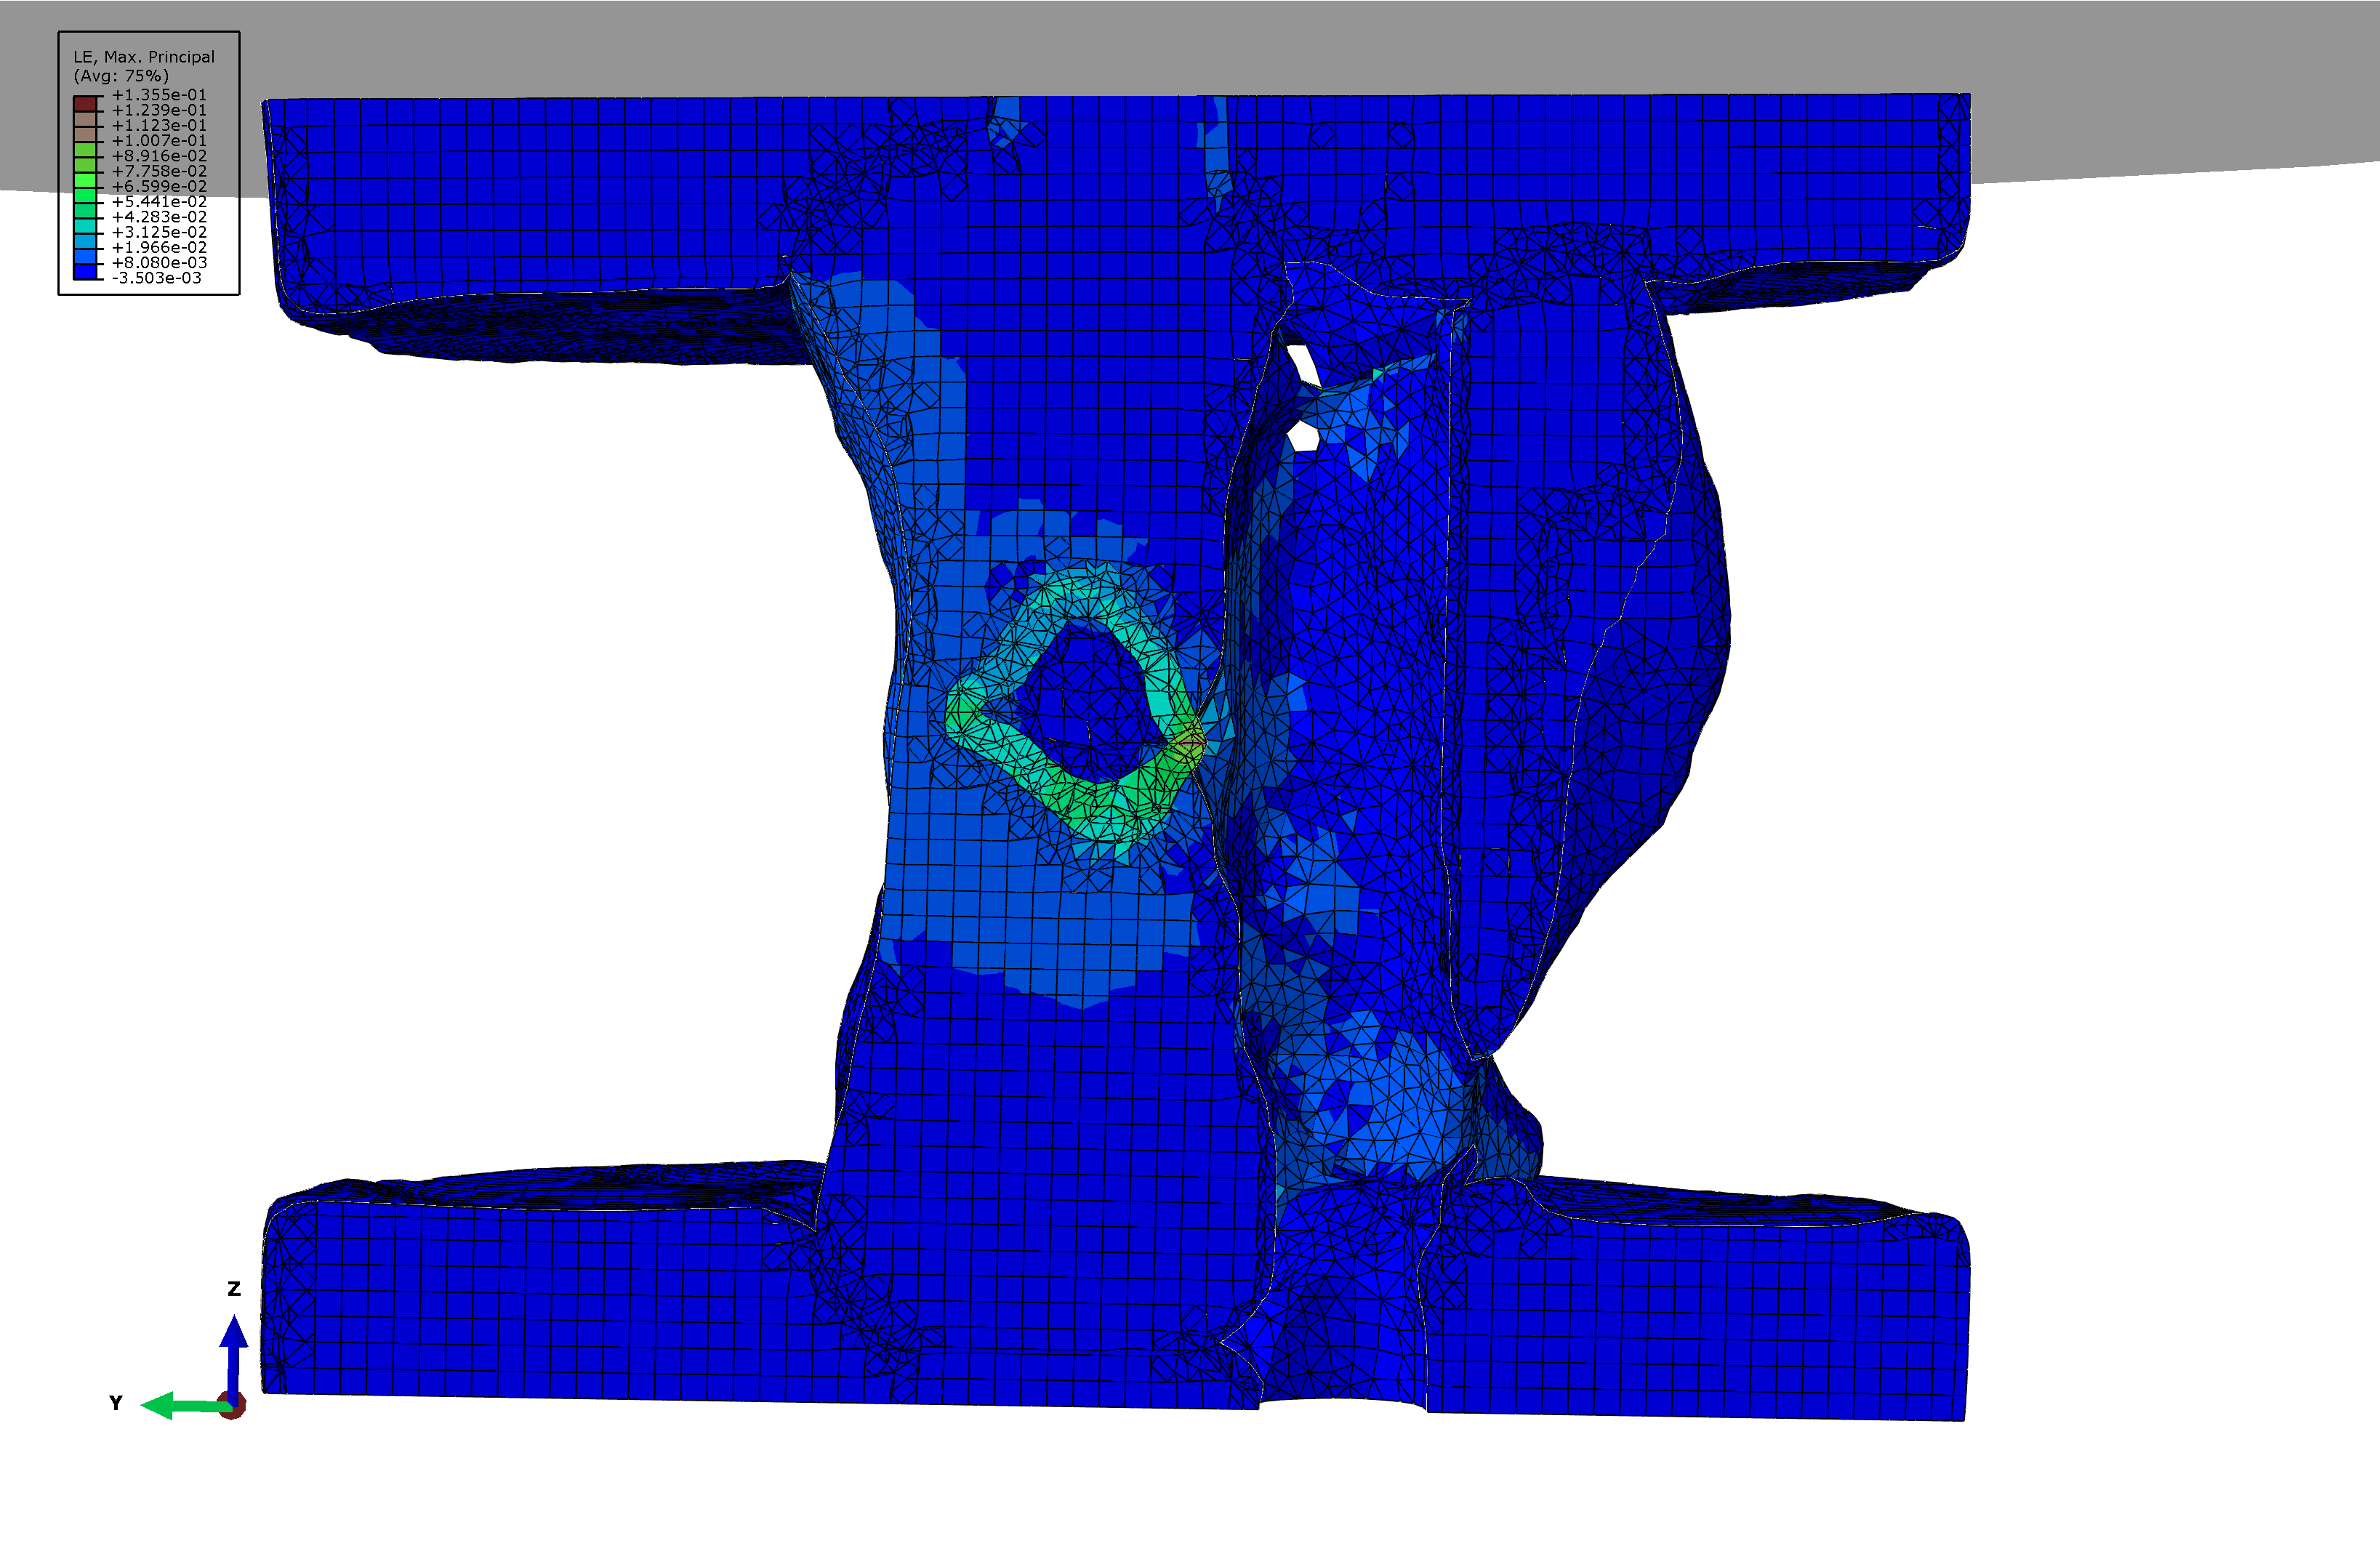
\includegraphics[width=10cm]{images/T2_CC1_postVP_Interface_ABAQUS_All_Side_Strain.png}   & T2 CC1  \begin{itemize} \item Experimental: 	1973.8	N/mm \item Computational:	2679.83 N/mm \item 2.8 \% Fill \end{itemize} \\ \hline 
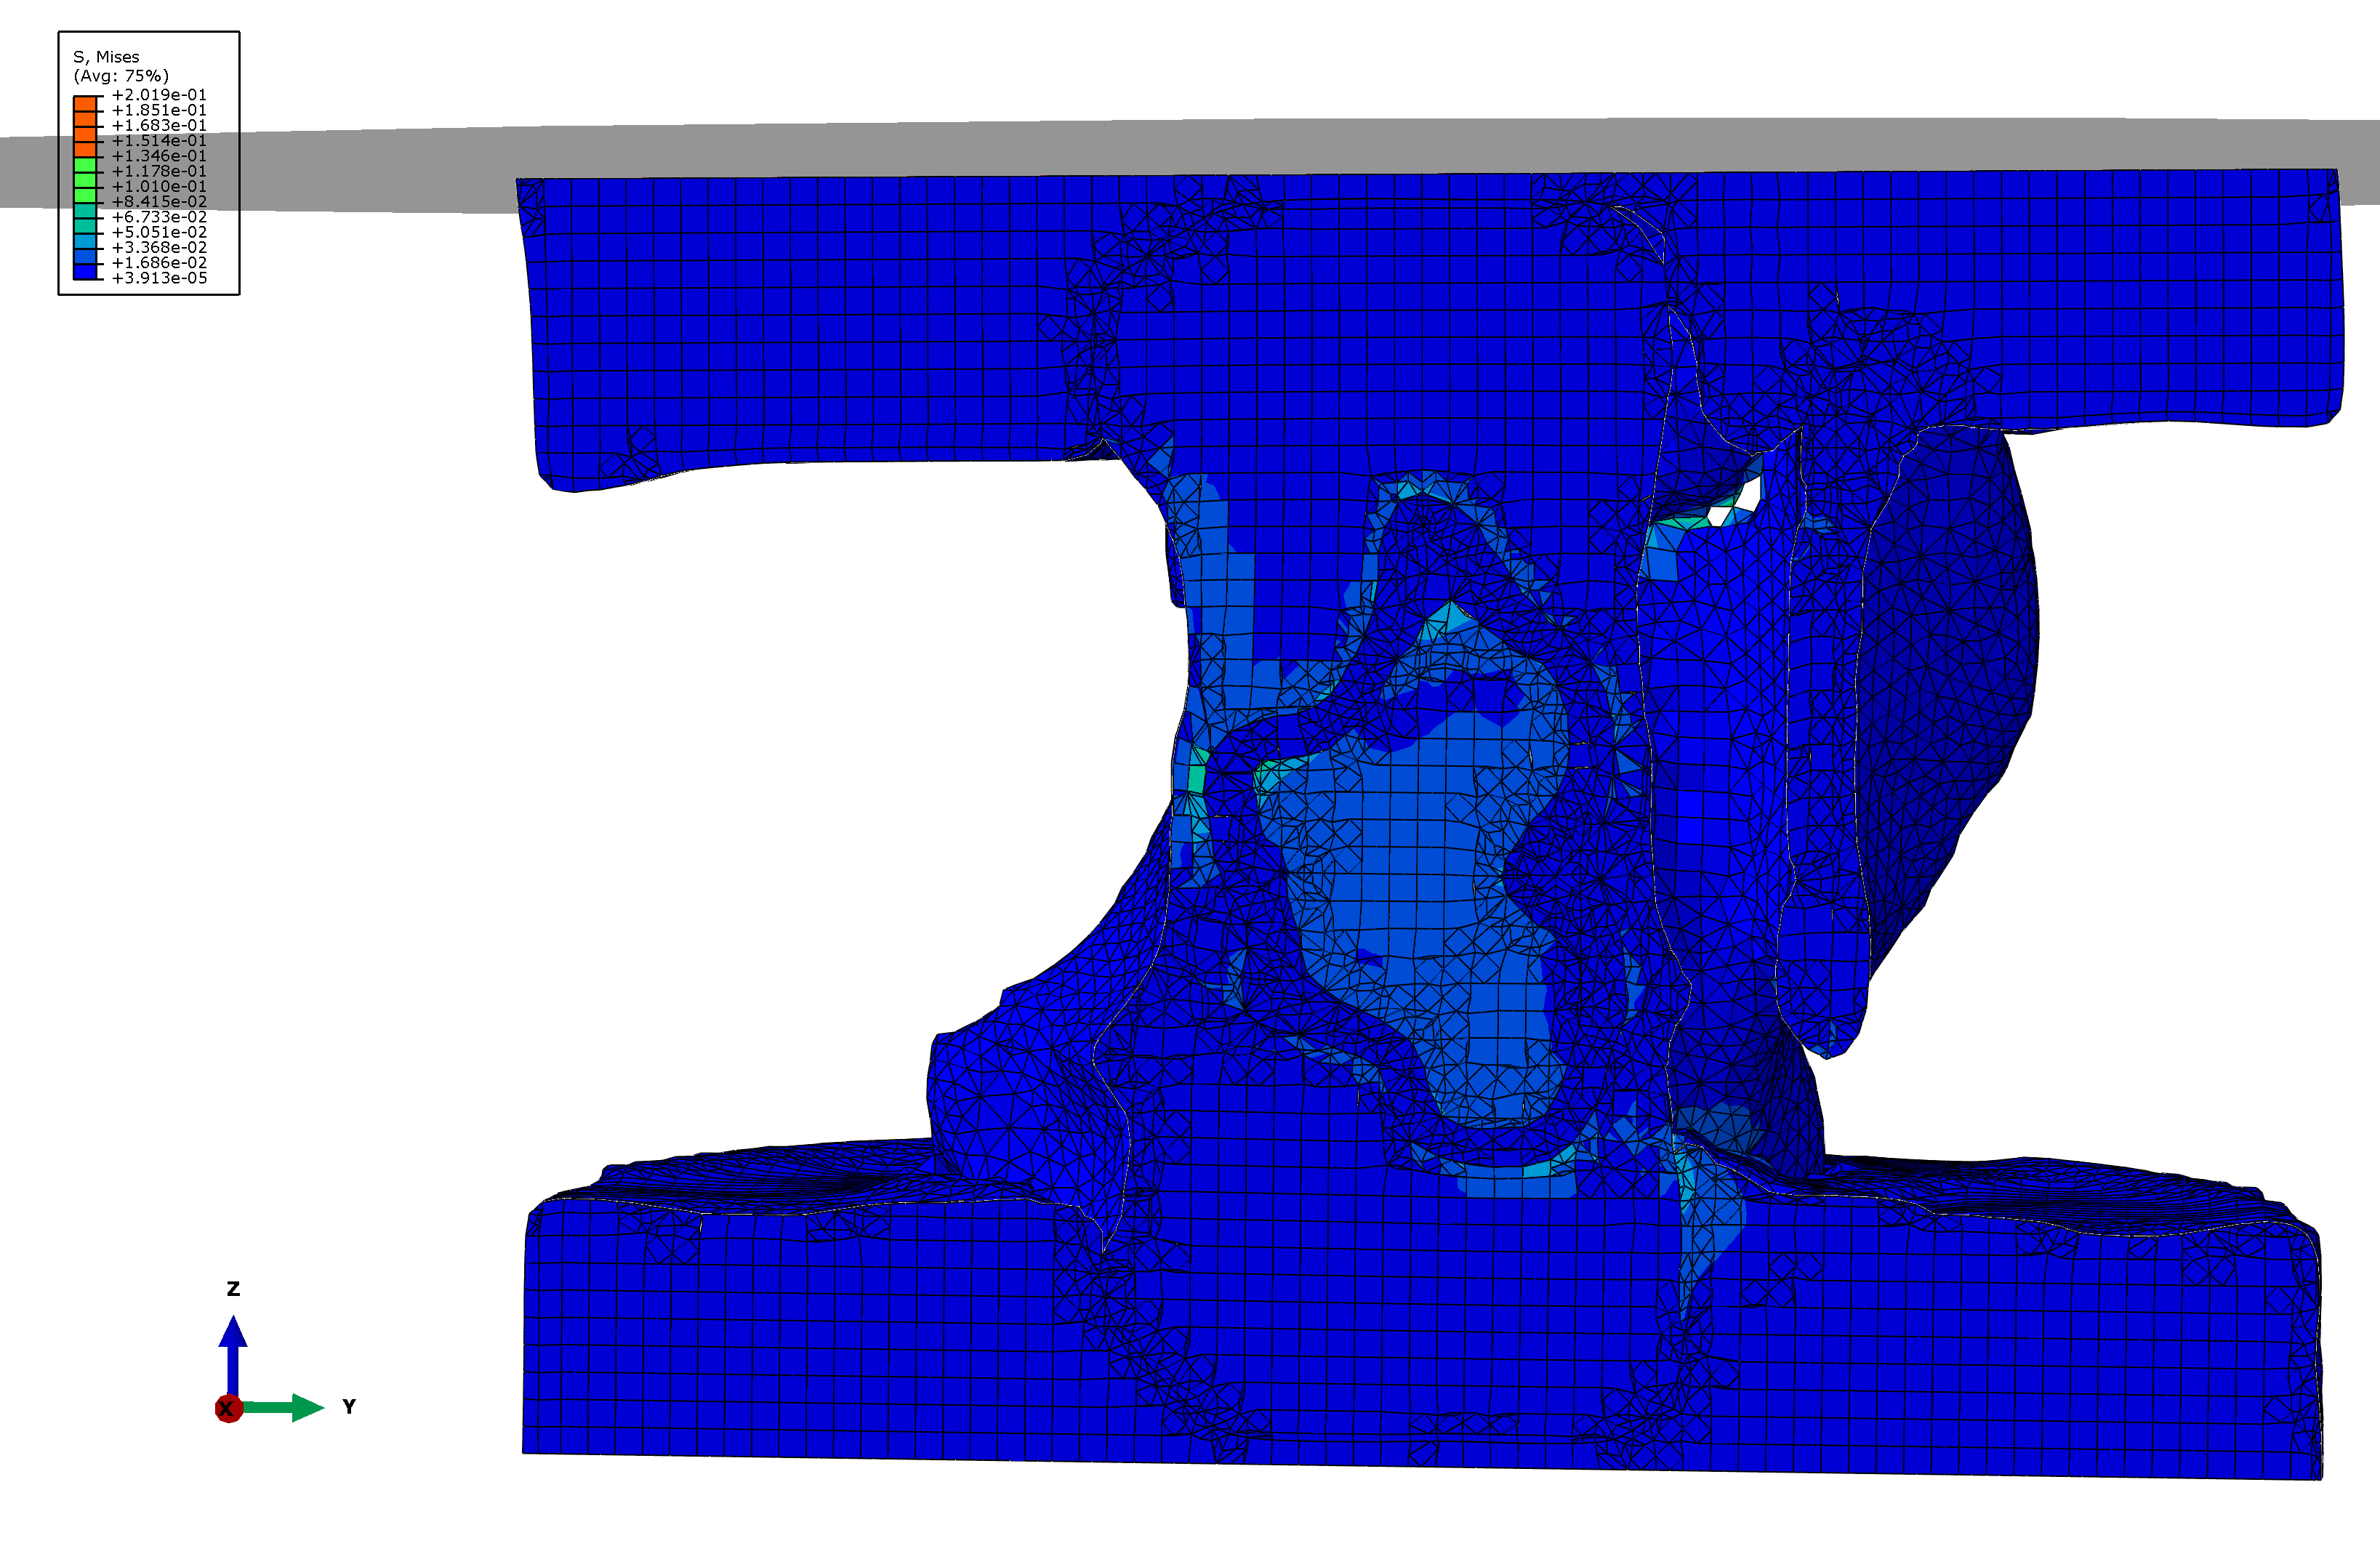
\includegraphics[width=10cm]{images/T2_CC2_postVP_Interface_ABAQUS_All_Side_Stress.png}   & 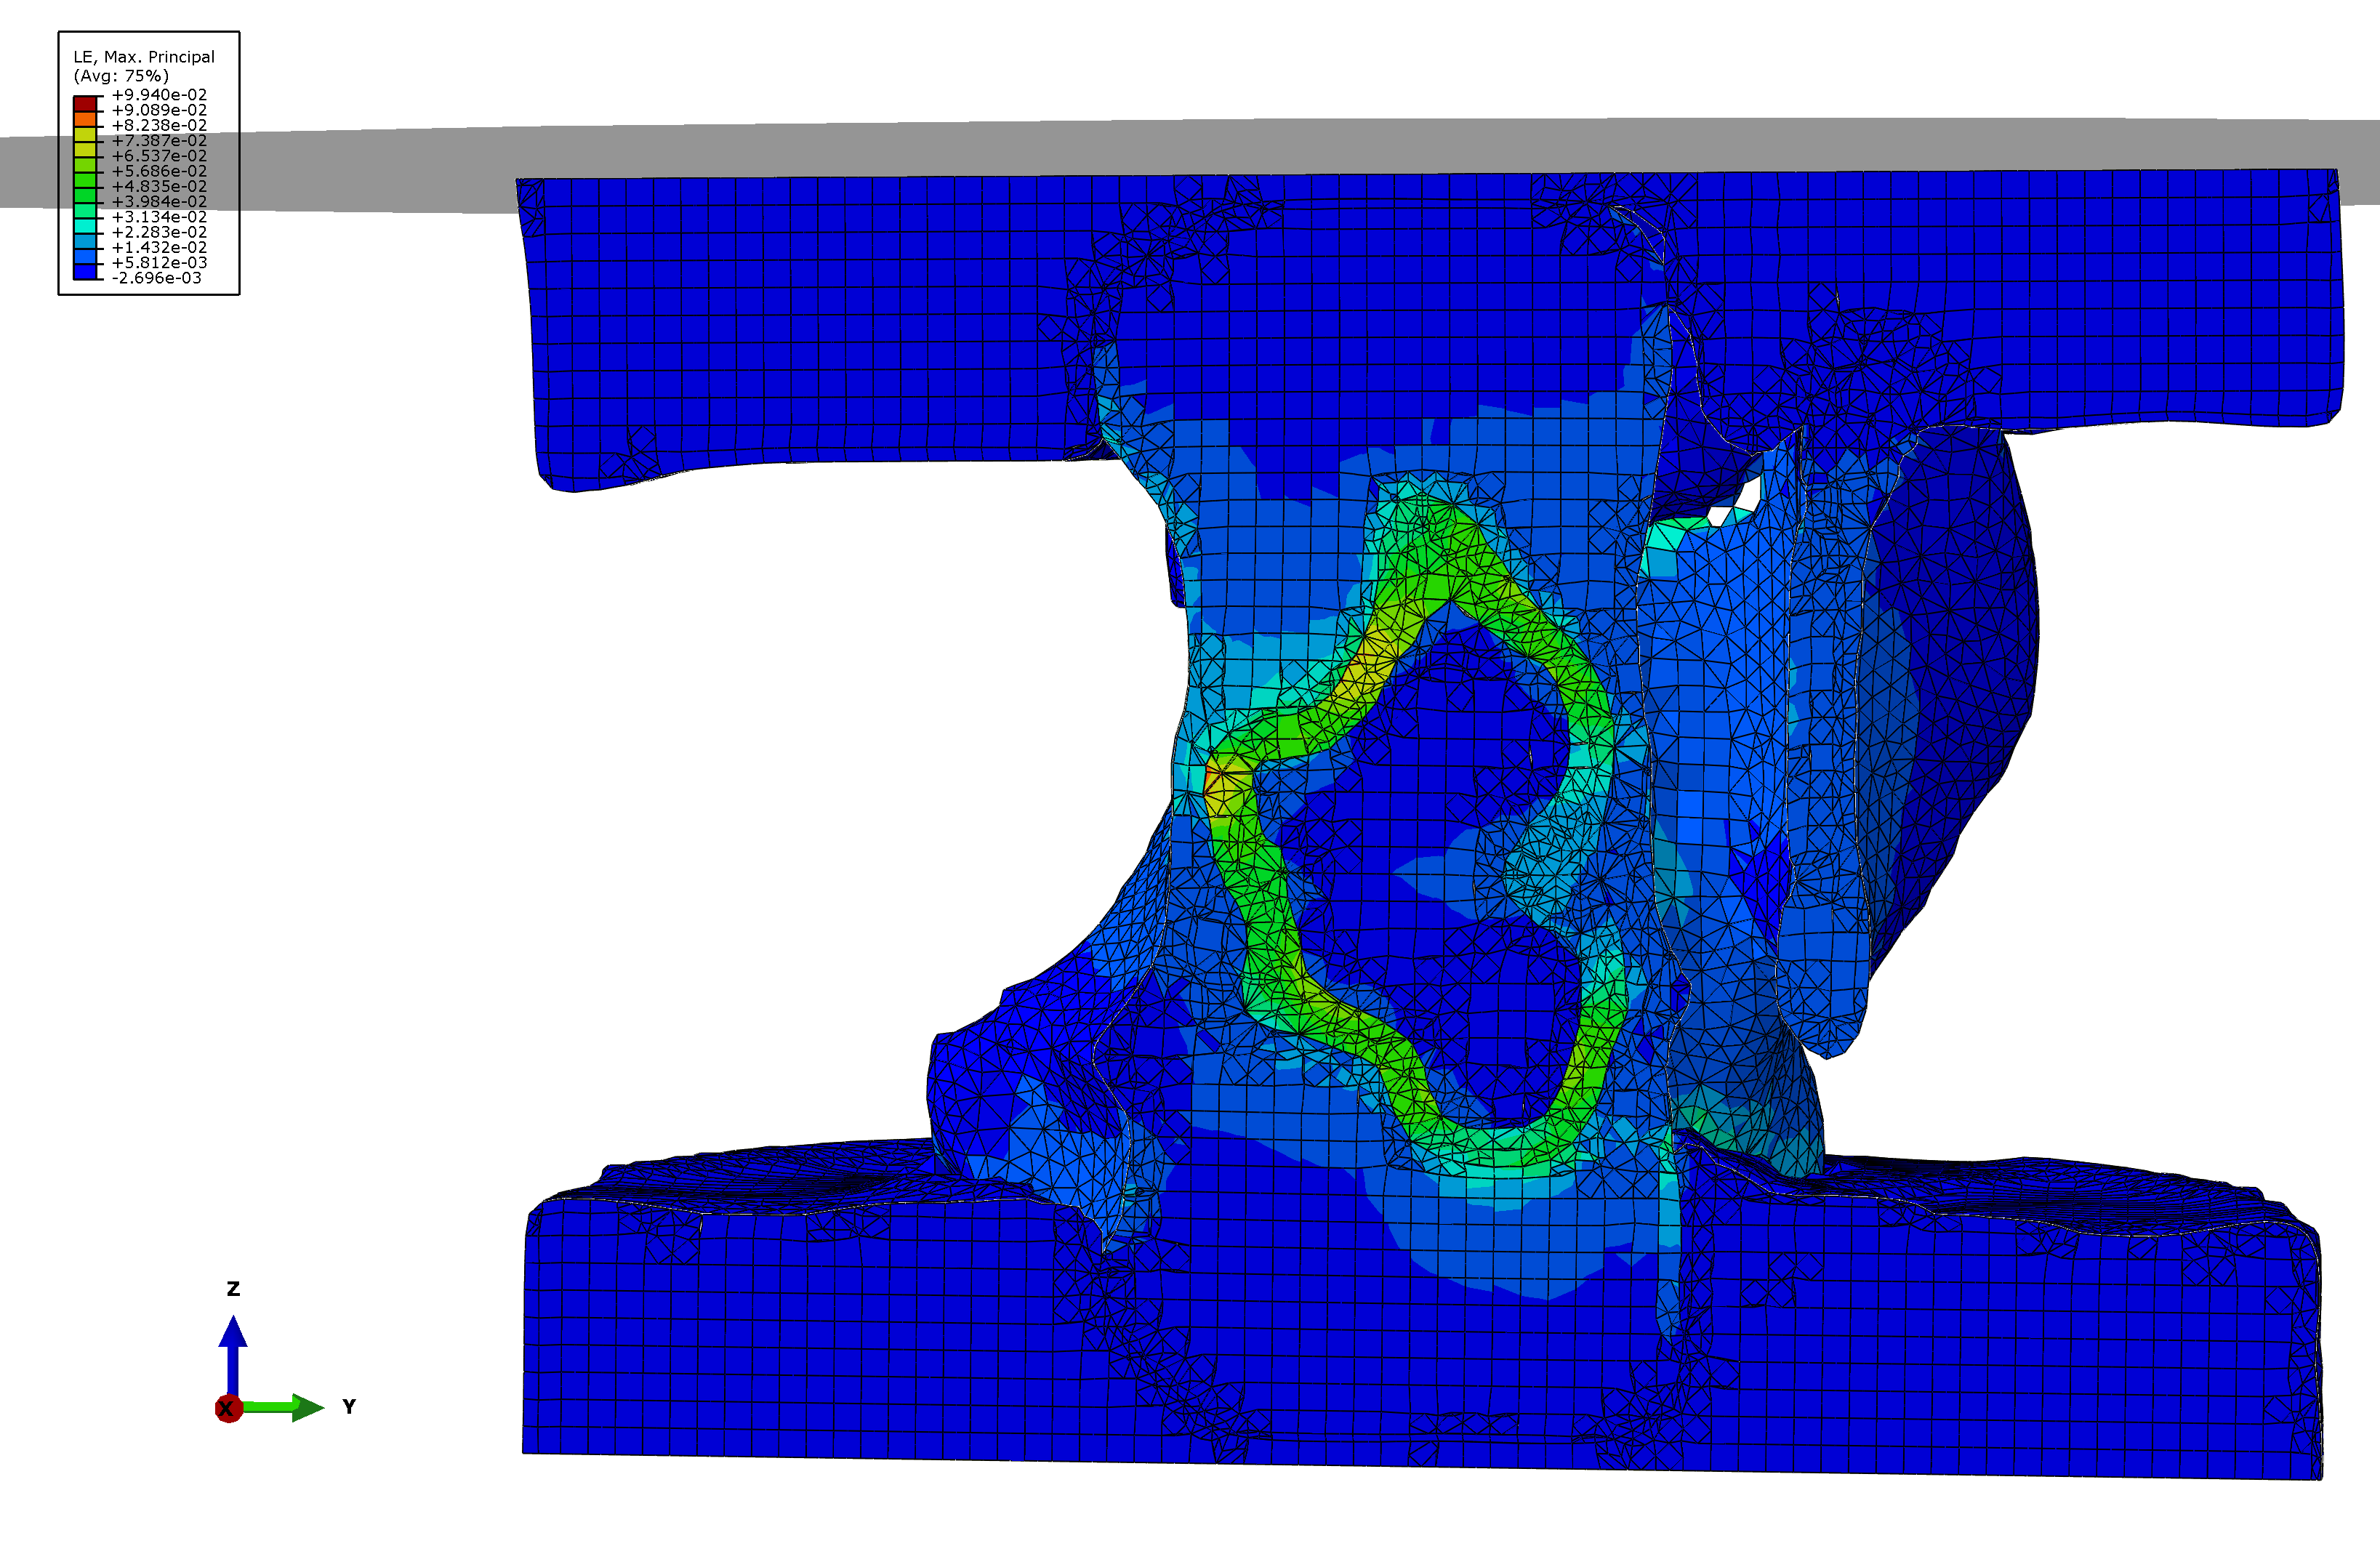
\includegraphics[width=10cm]{images/T2_CC2_postVP_Interface_ABAQUS_All_Side_Strain.png}   & T2 CC2  \begin{itemize} \item Experimental: 	3644.2	N/mm \item Computational:	3854.7 N/mm \item 14.3\% Fill \end{itemize} \\ \hline 
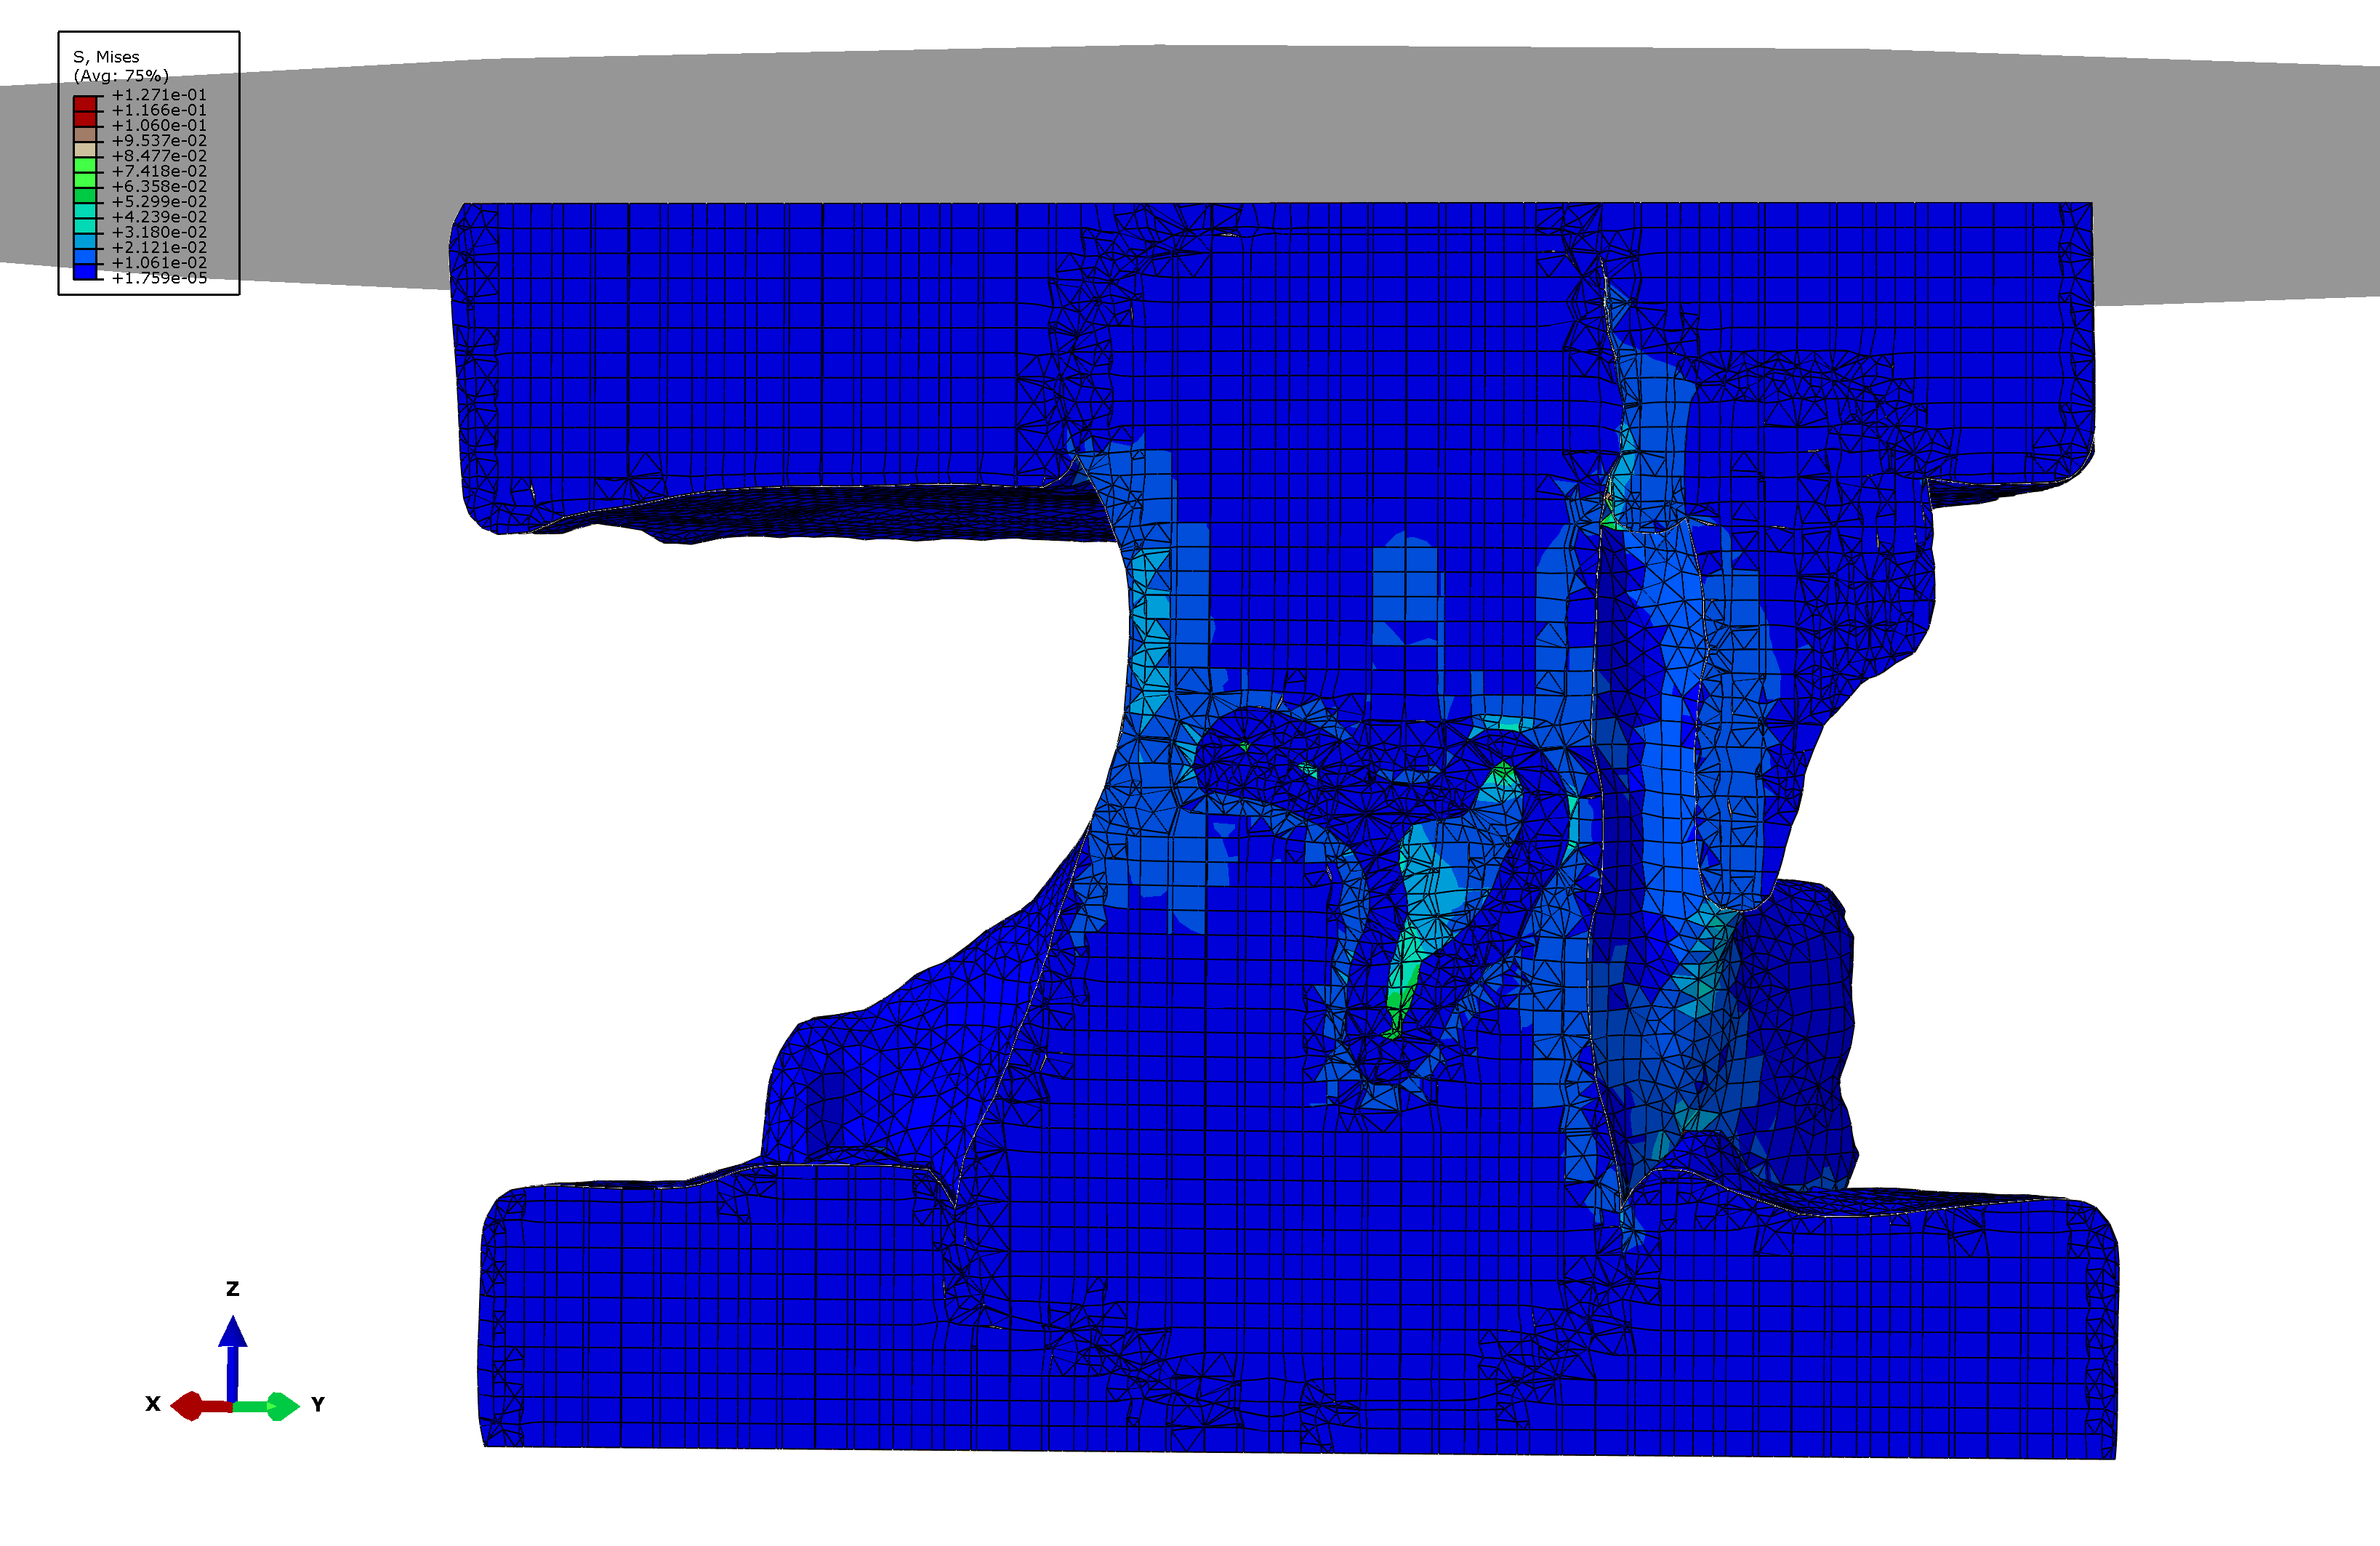
\includegraphics[width=10cm]{images/T4_CC3_postVP_Interface_ABAQUS_All_Side_Stress.png}   & 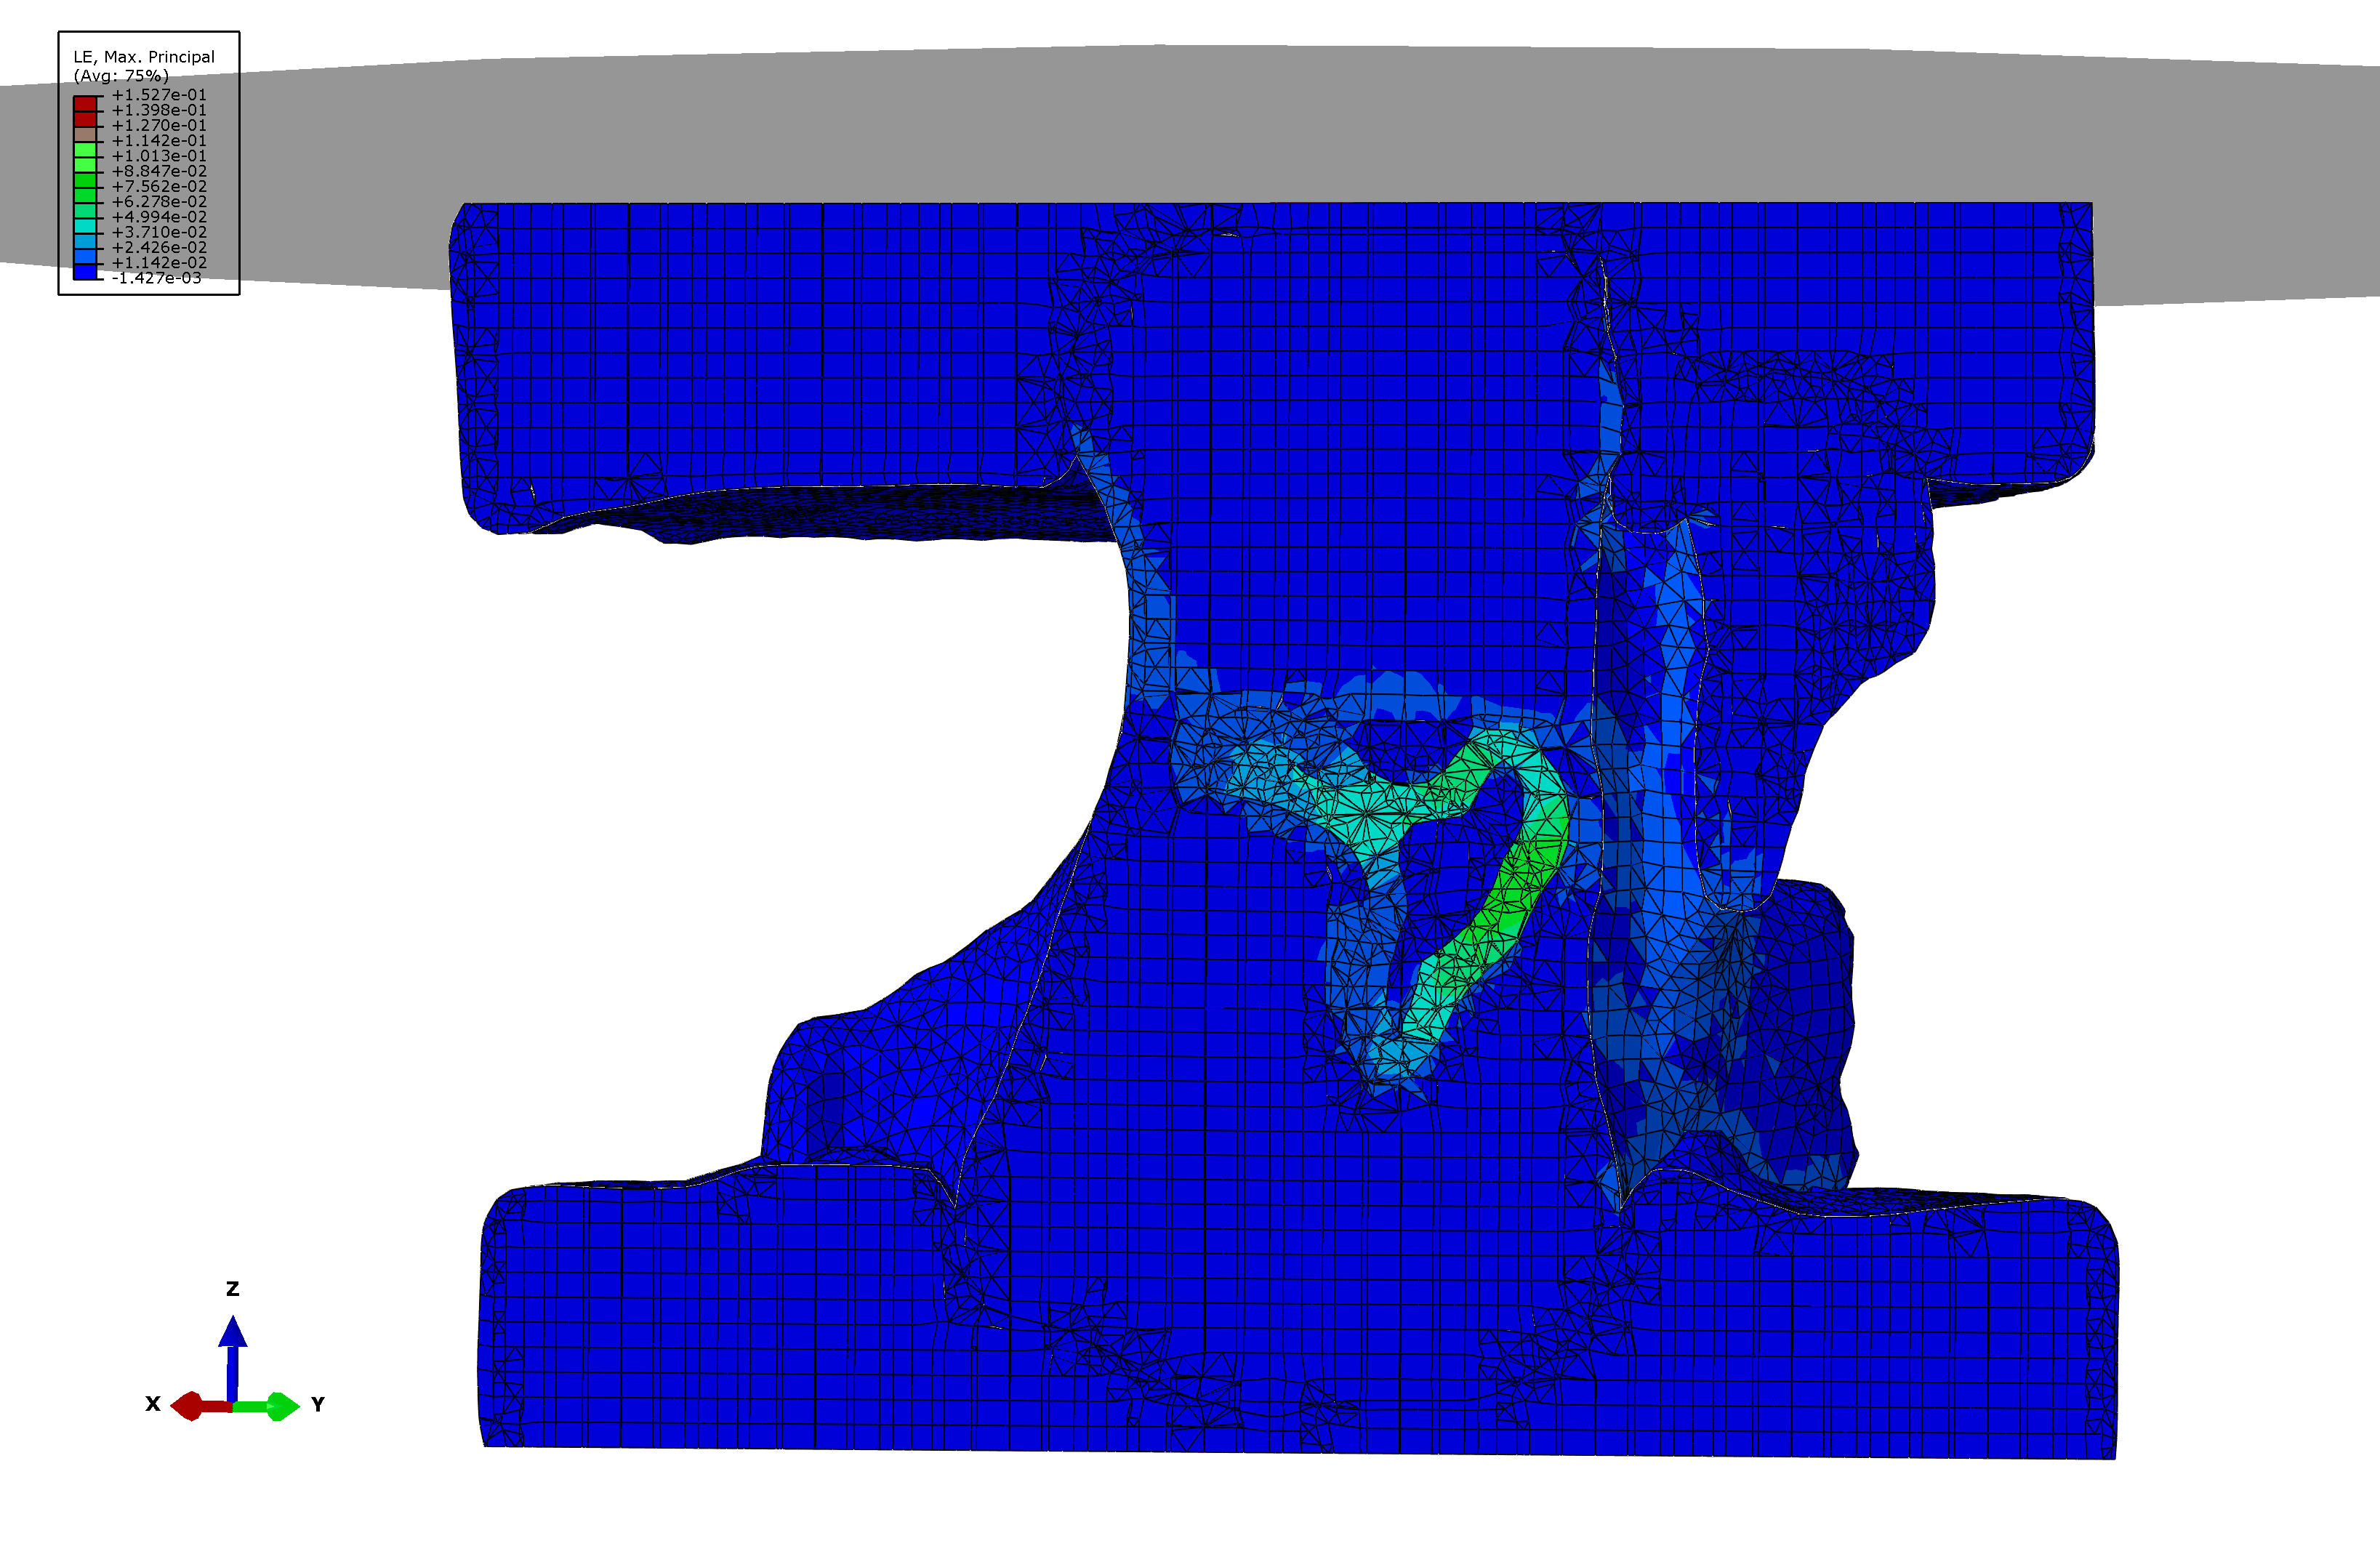
\includegraphics[width=10cm]{images/T4_CC3_postVP_Interface_ABAQUS_All_Side_Strain.png}   & T4 CC3  \begin{itemize} \item Experimental: 	2838.5	N/mm \item Computational:	3851.88
 N/mm \item 5.1 \% Fill \end{itemize} \\ \hline 
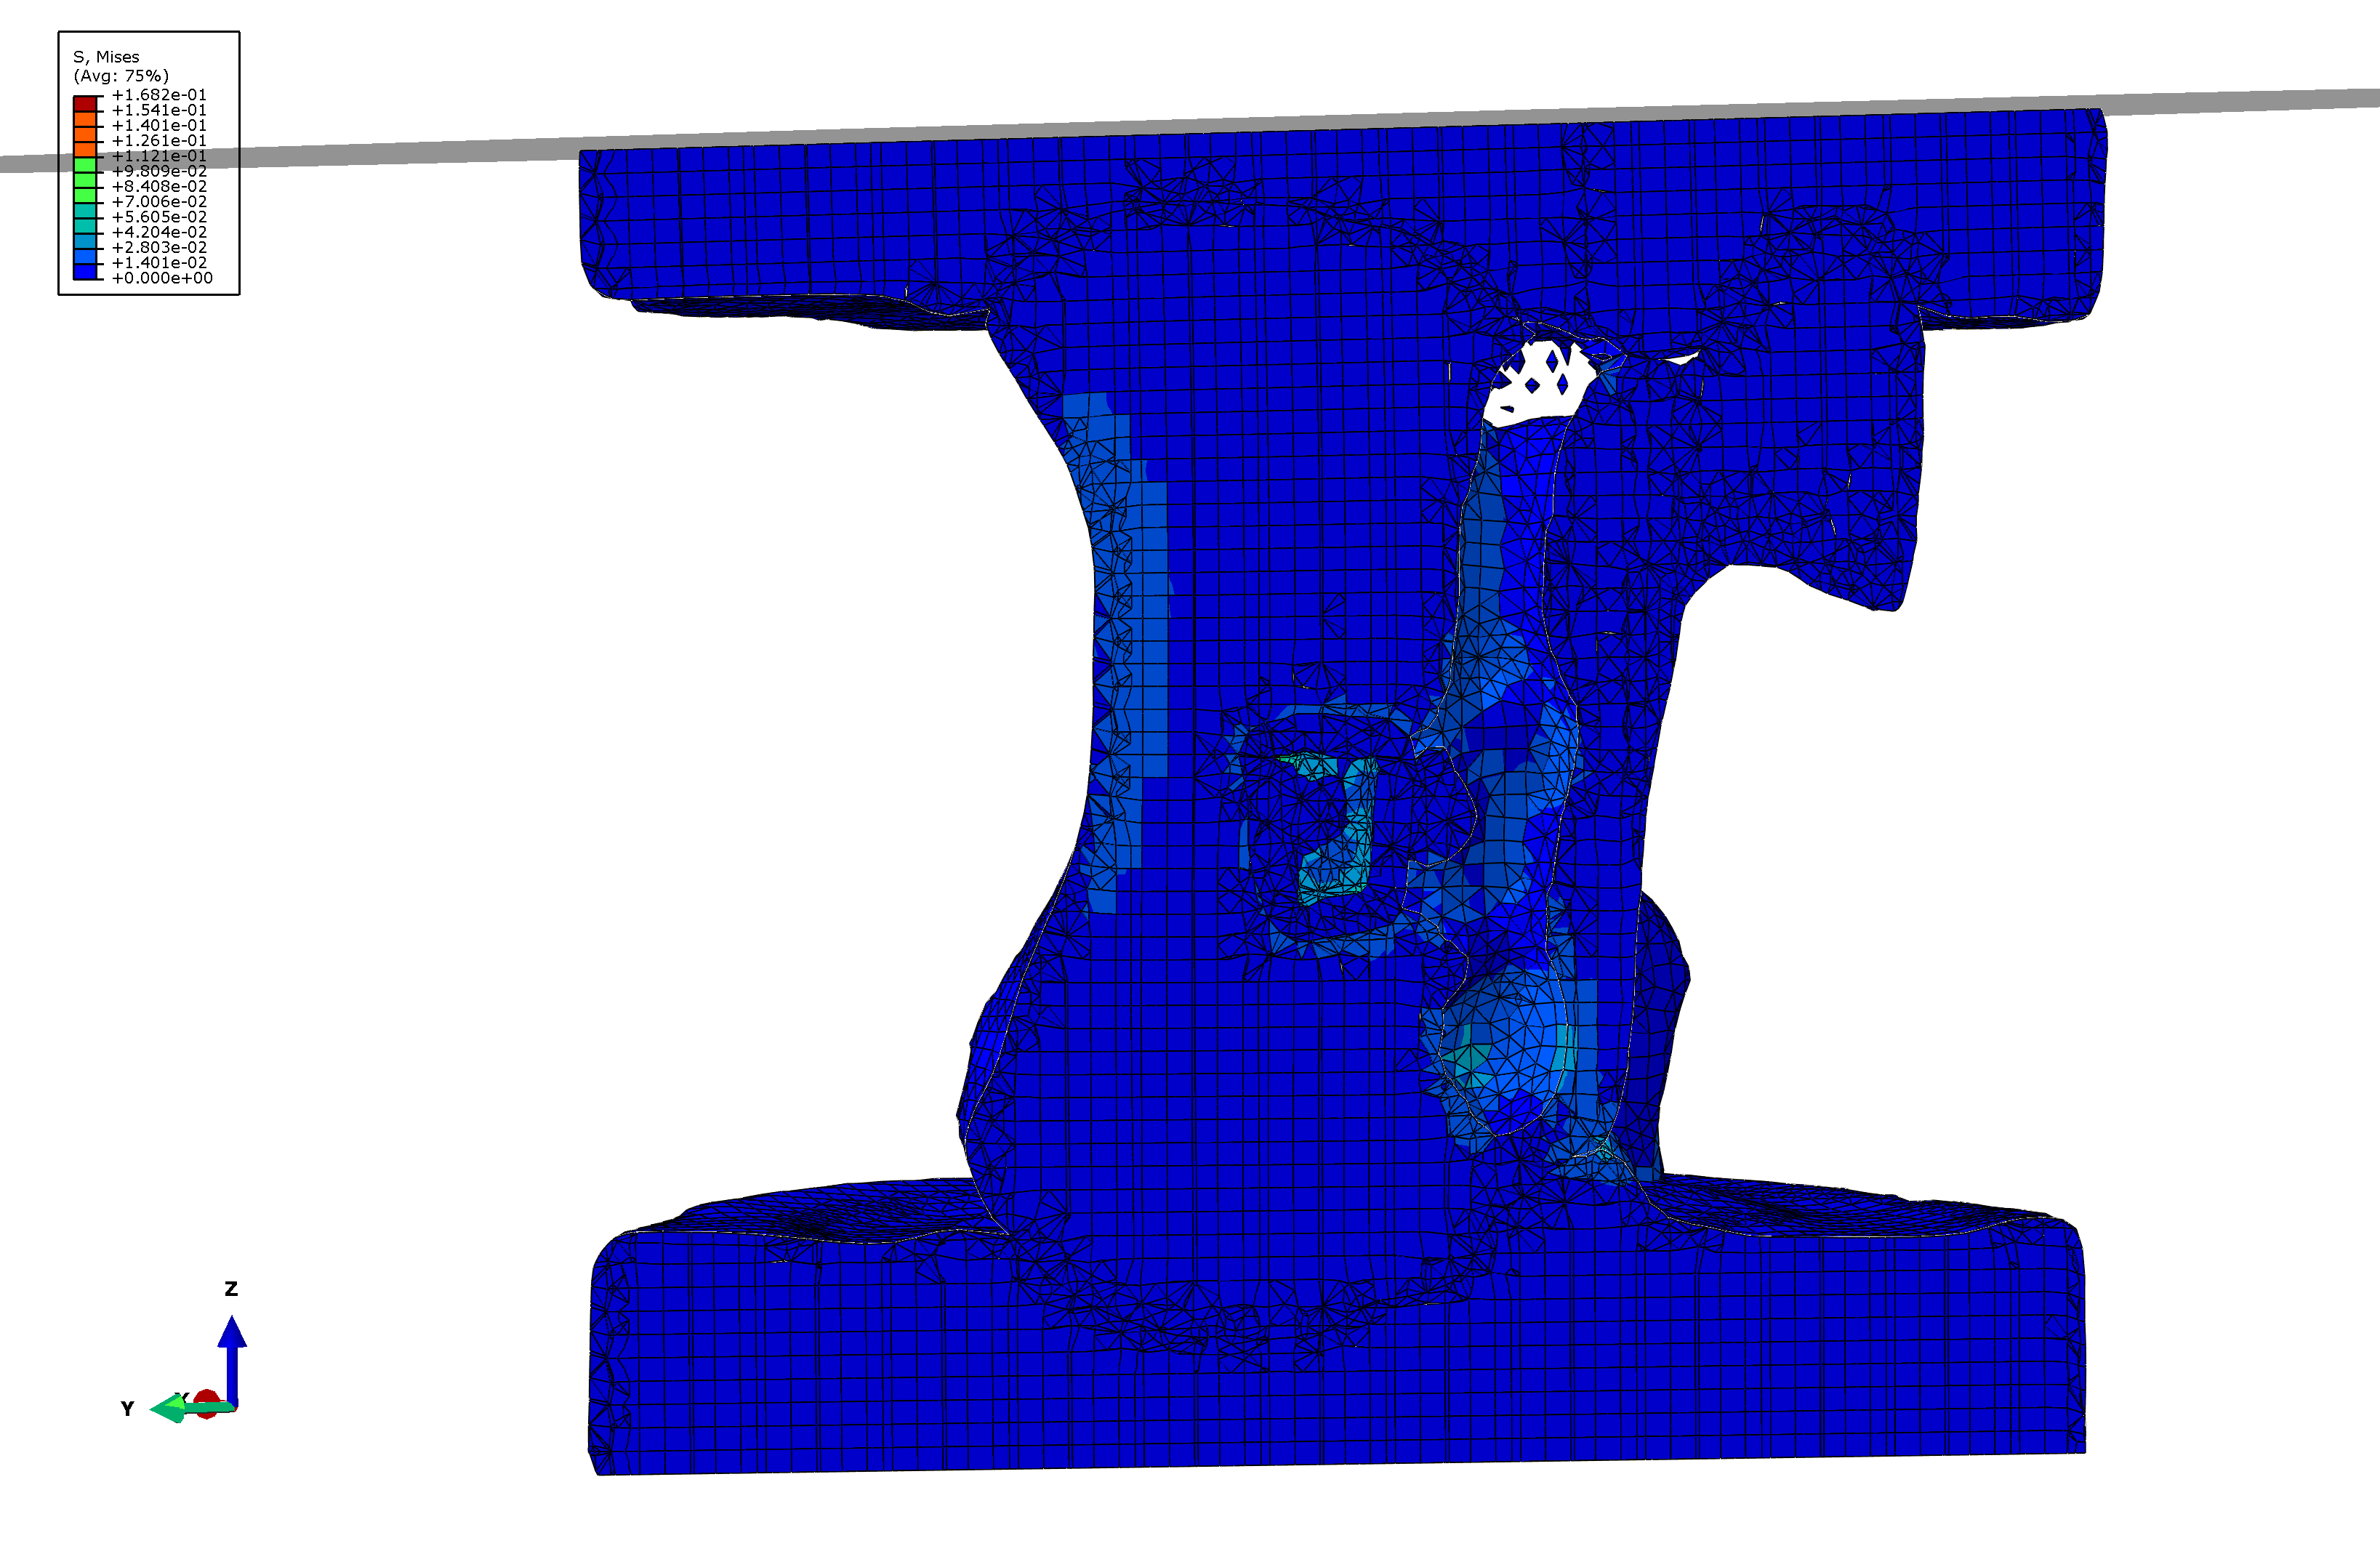
\includegraphics[width=10cm]{images/T6_CC1_postVP_Interface_ABAQUS_All_Side_Stress.png}   & 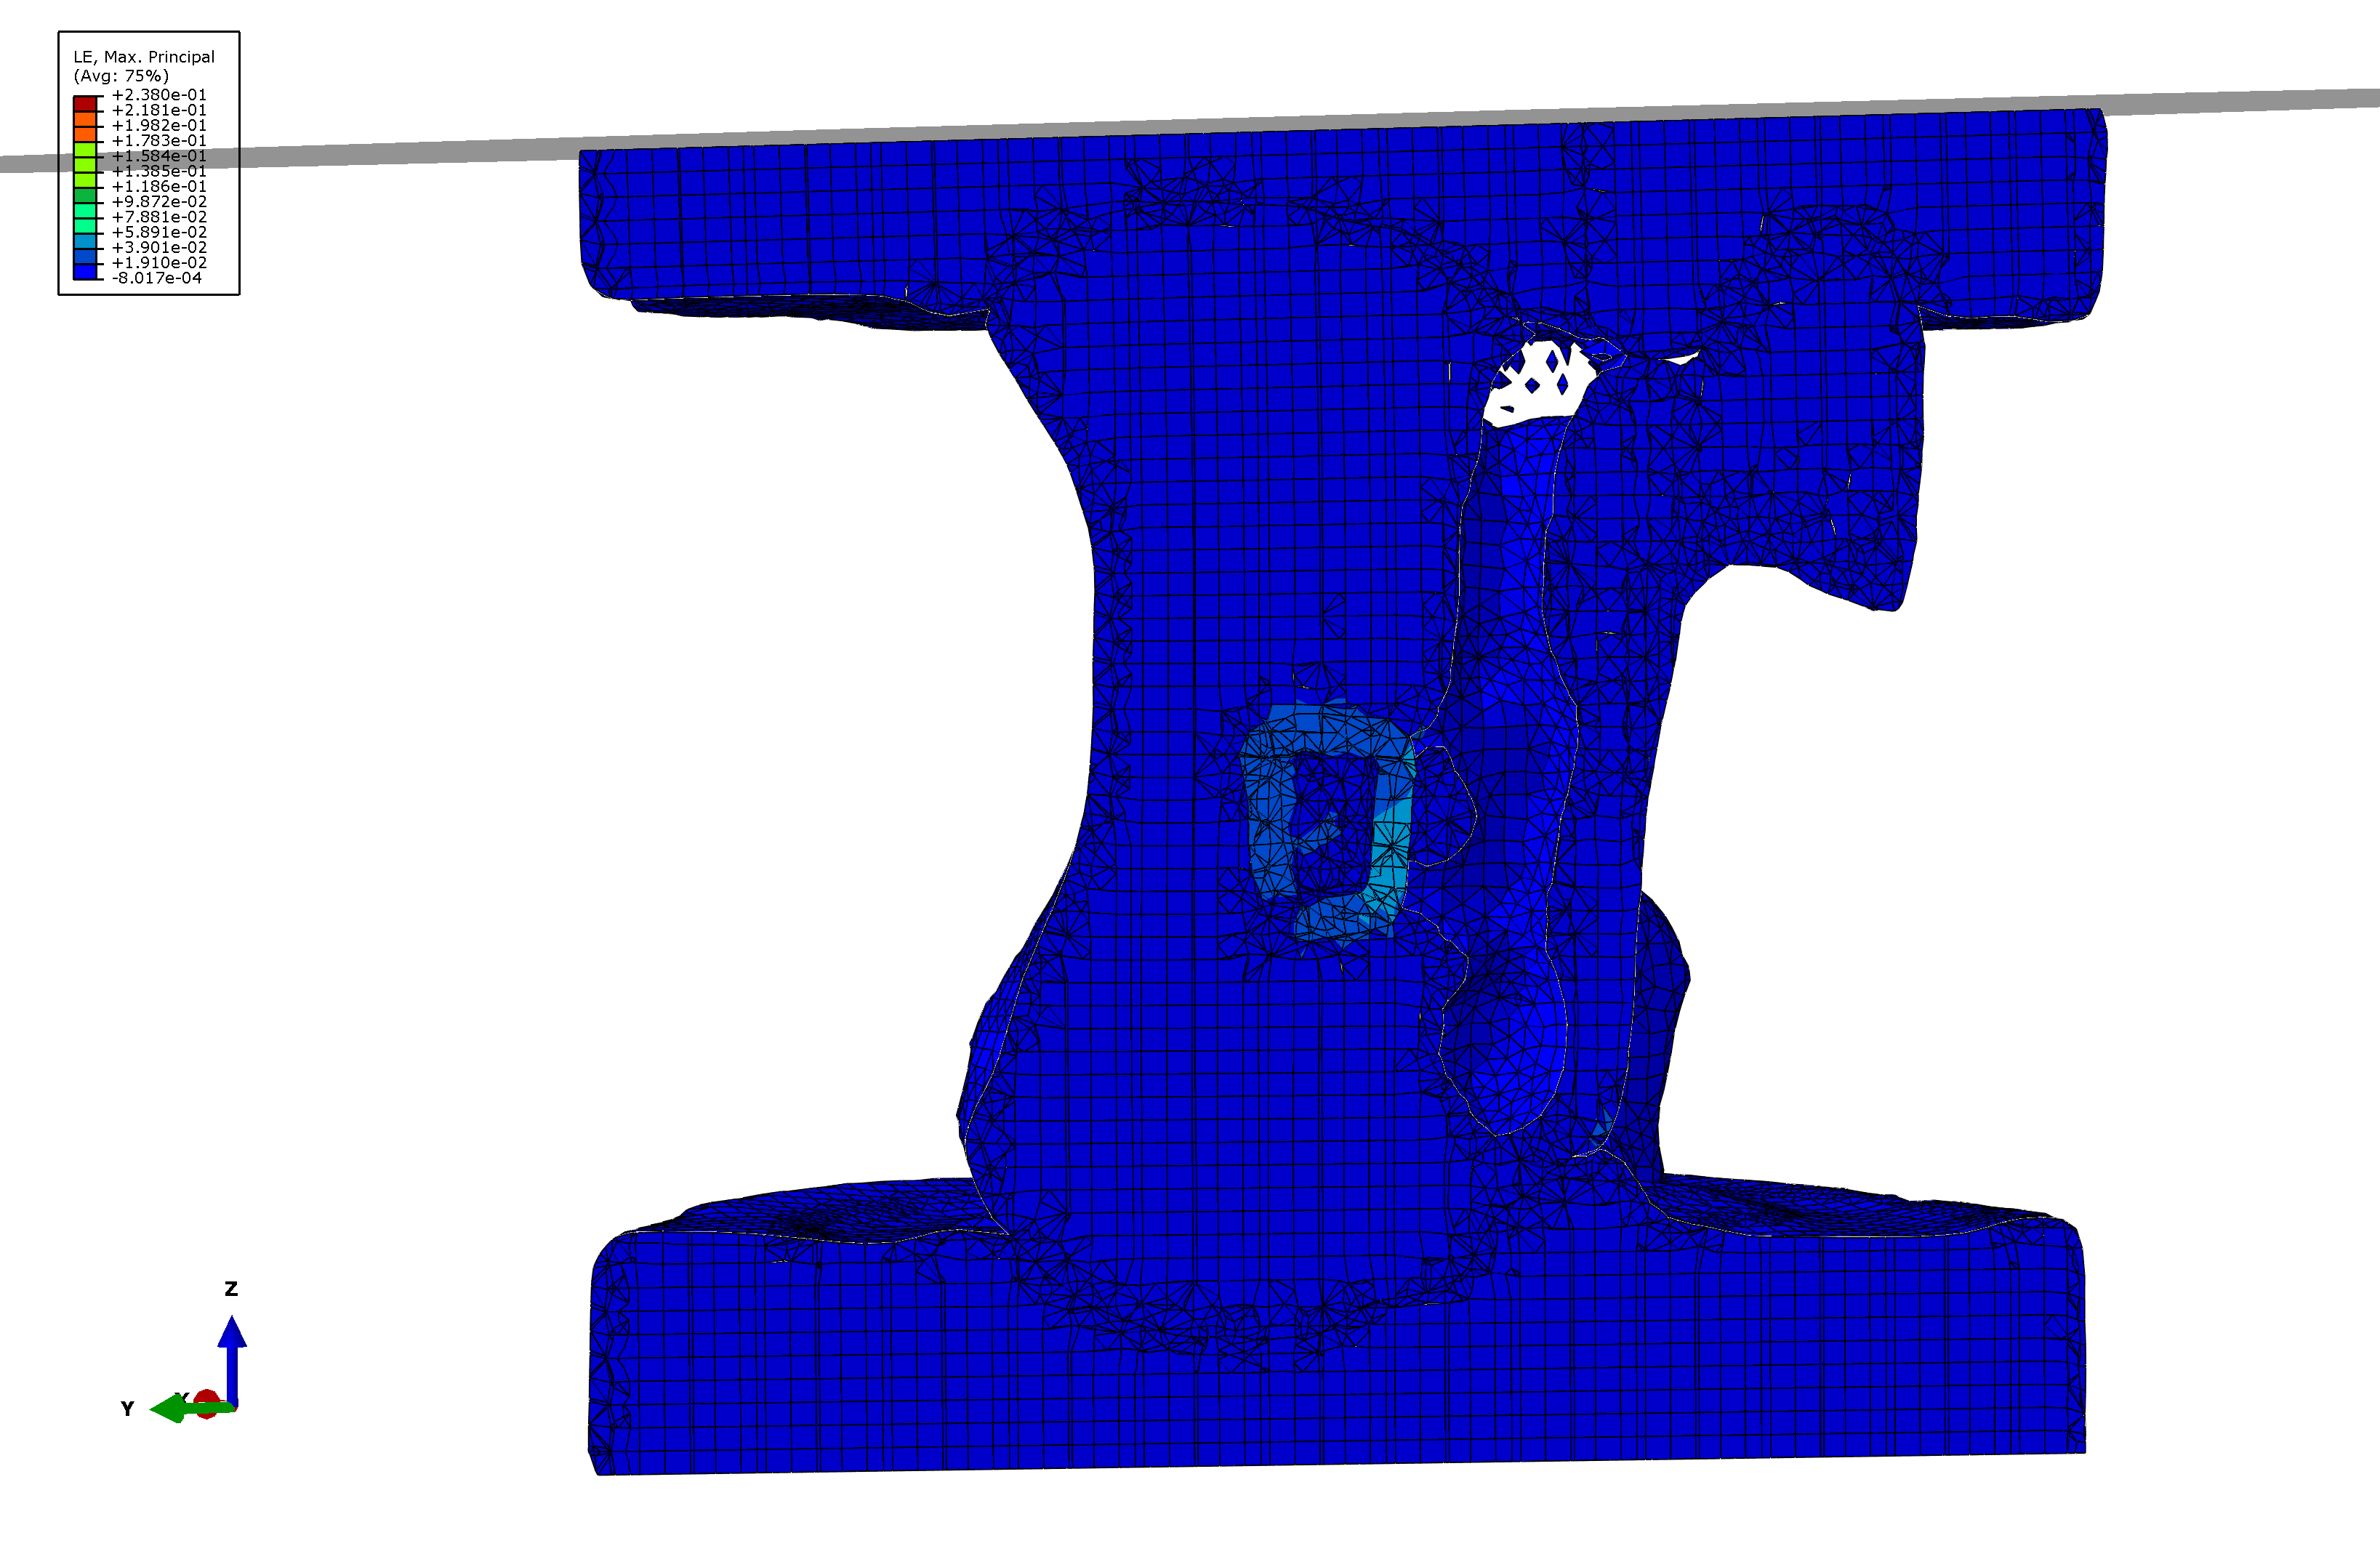
\includegraphics[width=10cm]{images/T6_CC1_postVP_Interface_ABAQUS_All_Side_Strain.png}   & T6 CC1  \begin{itemize} \item Experimental: 	3142.1	N/mm \item Computational:	2857.61 N/mm \item 2.8 \% Fill \end{itemize} \\ \hline 
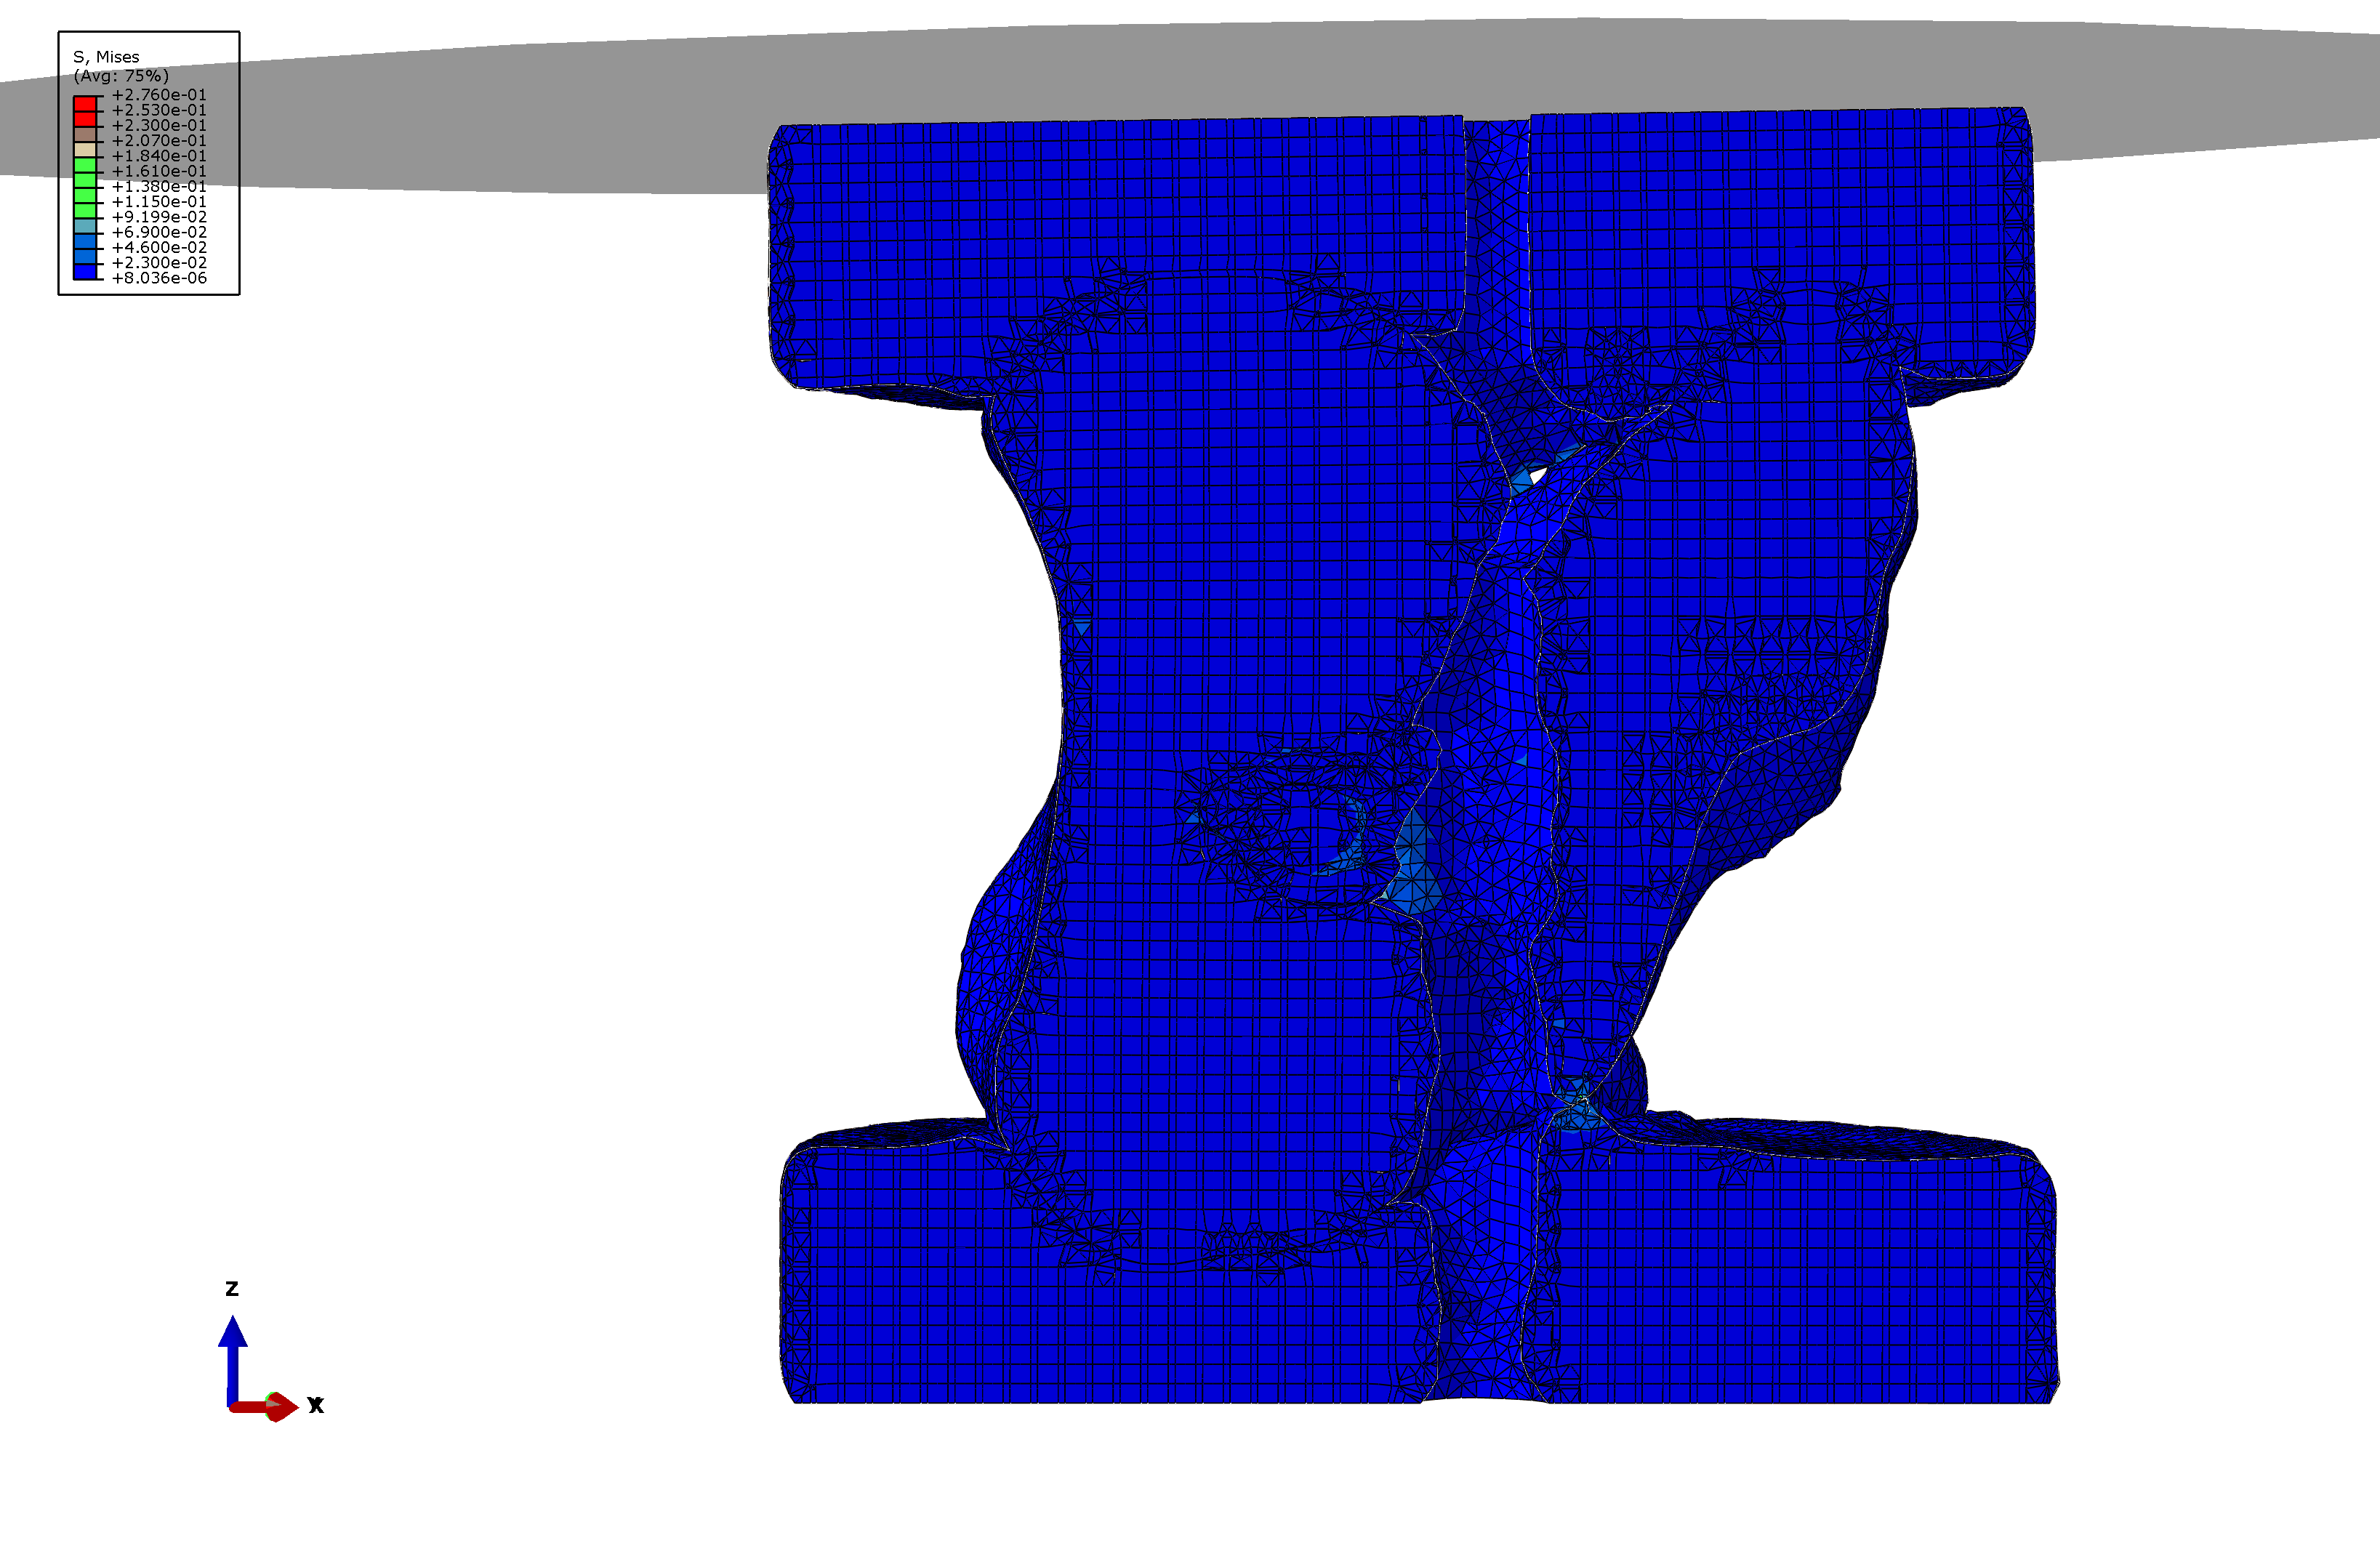
\includegraphics[width=10cm]{images/T8_CC1_postVP_Interface_ABAQUS_All_Side_Stress.png}   & 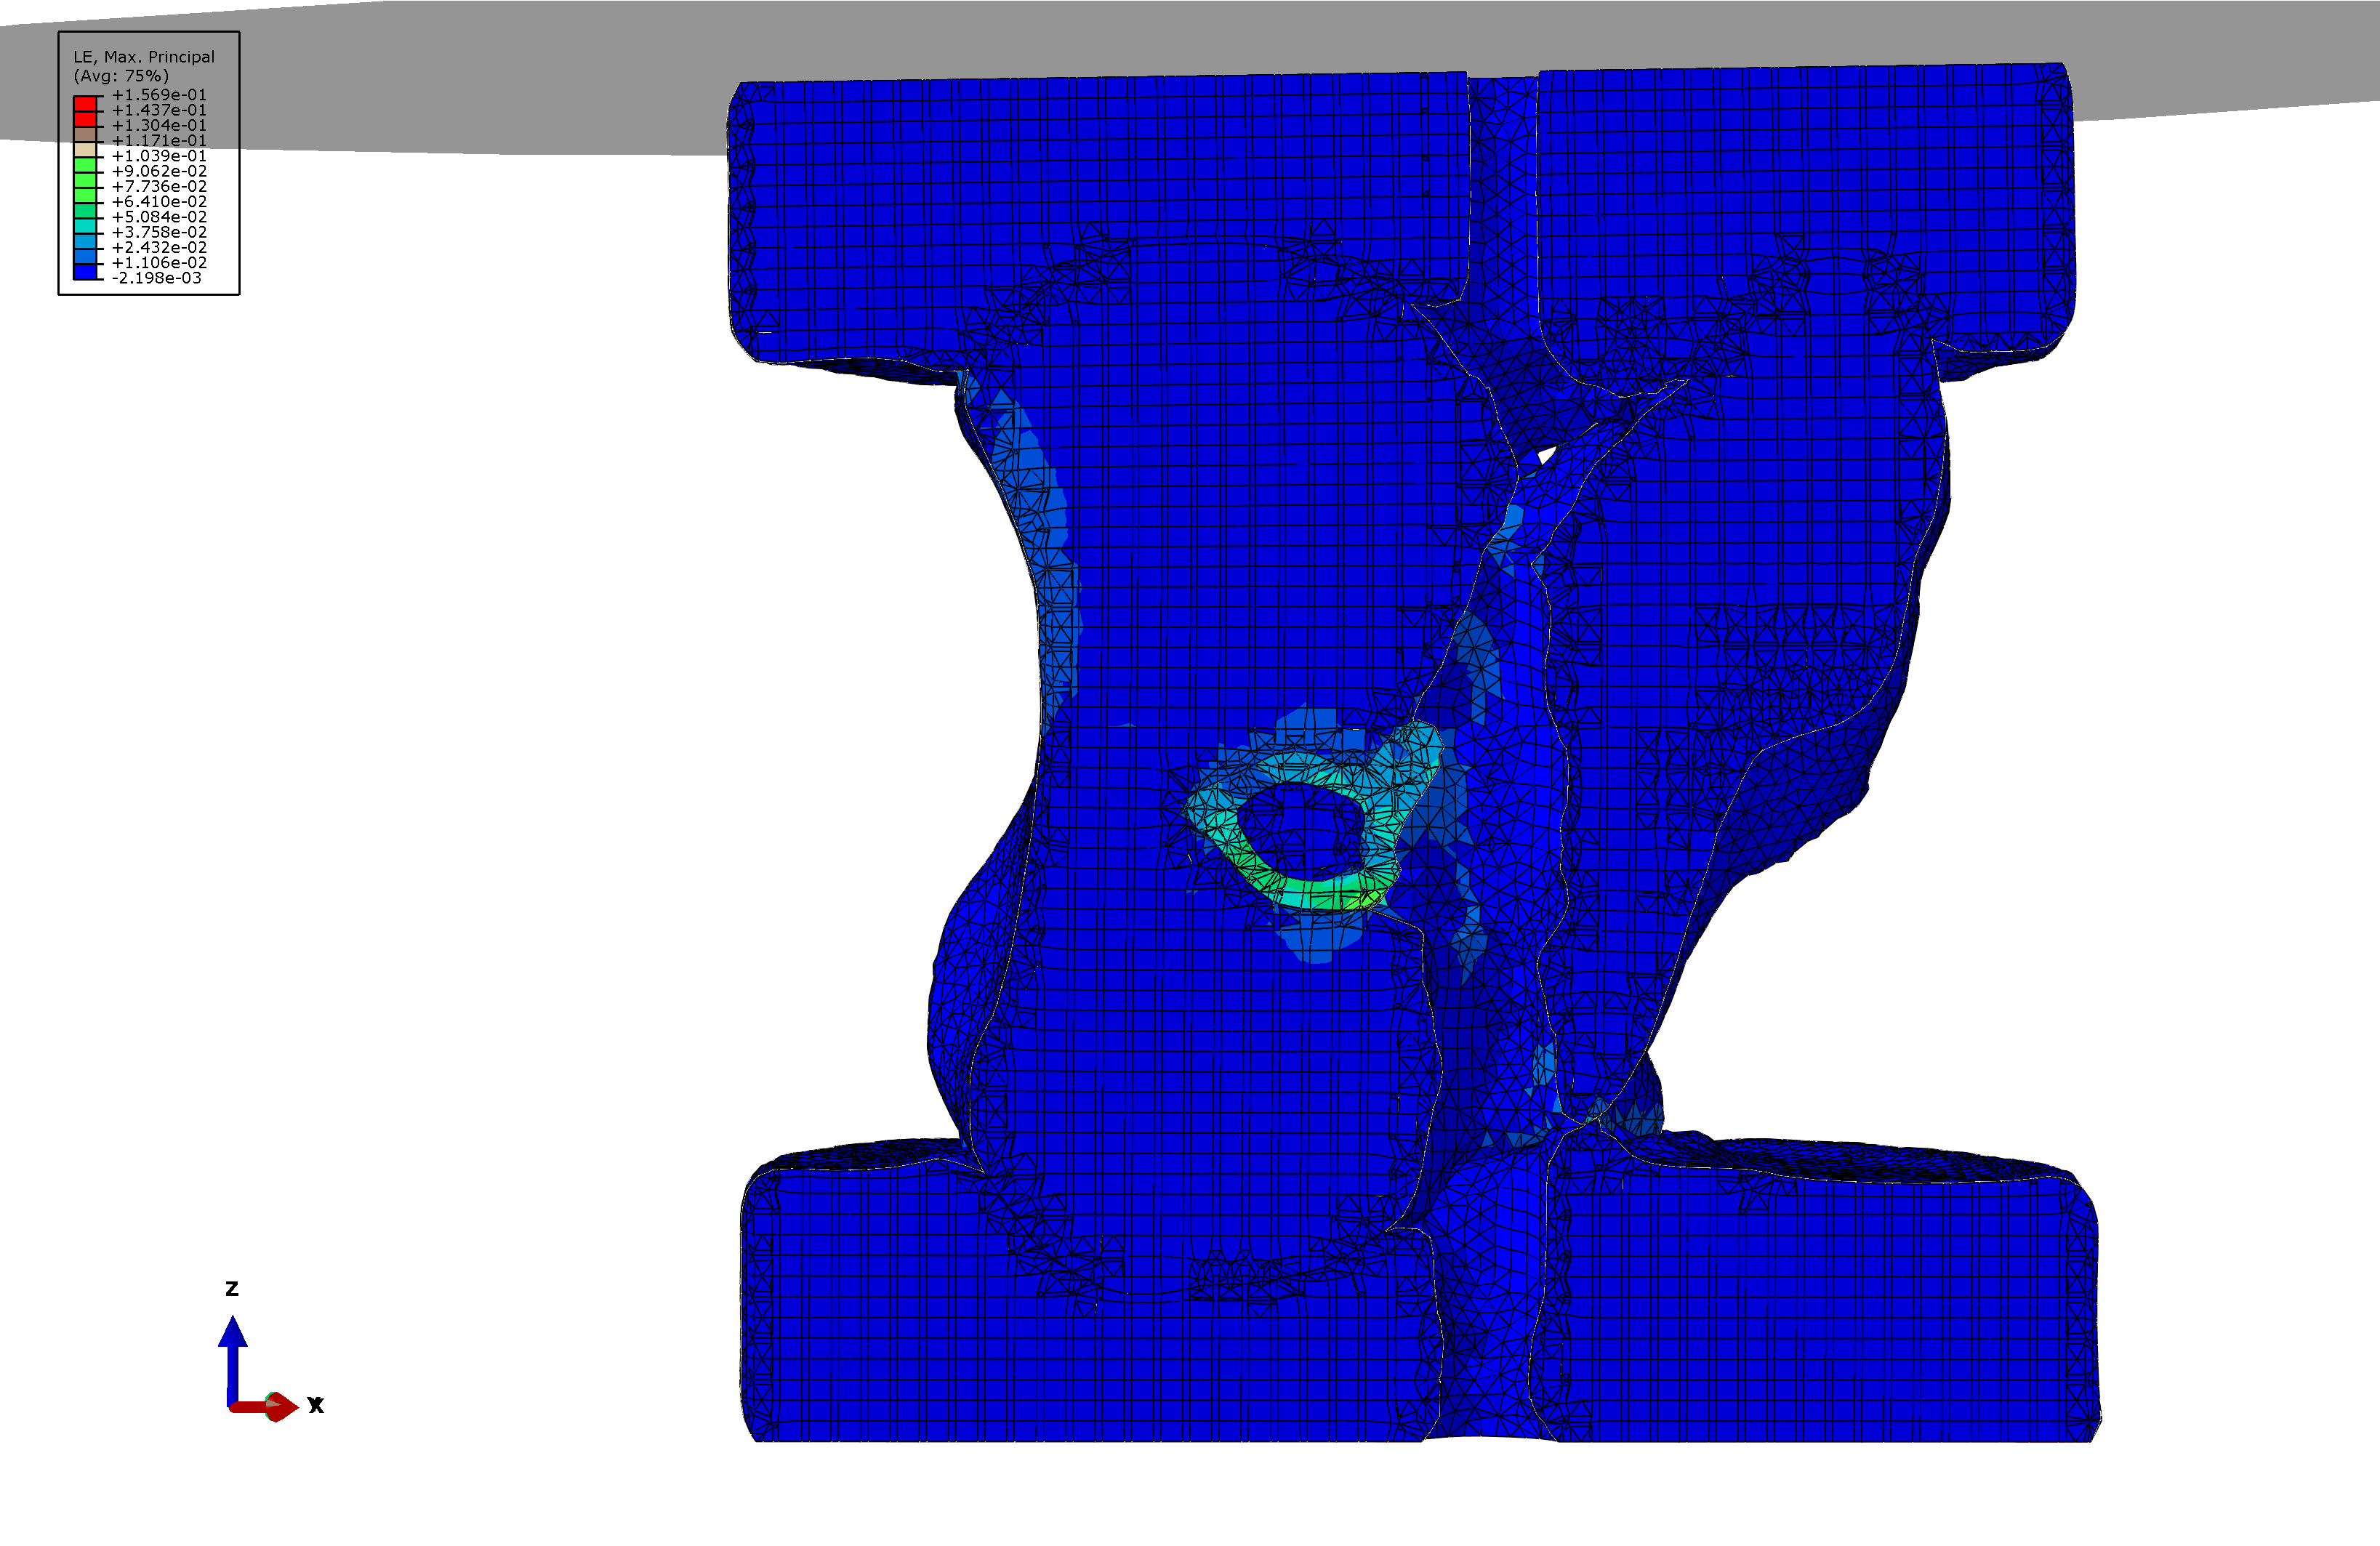
\includegraphics[width=10cm]{images/T8_CC1_postVP_Interface_ABAQUS_All_Side_Strain.png}   & T8 CC1  \begin{itemize} \item Experimental: 	4068.3	N/mm \item Computational:	4420.33
 N/mm \item 3.3 \% Fill \end{itemize} \\ \hline 
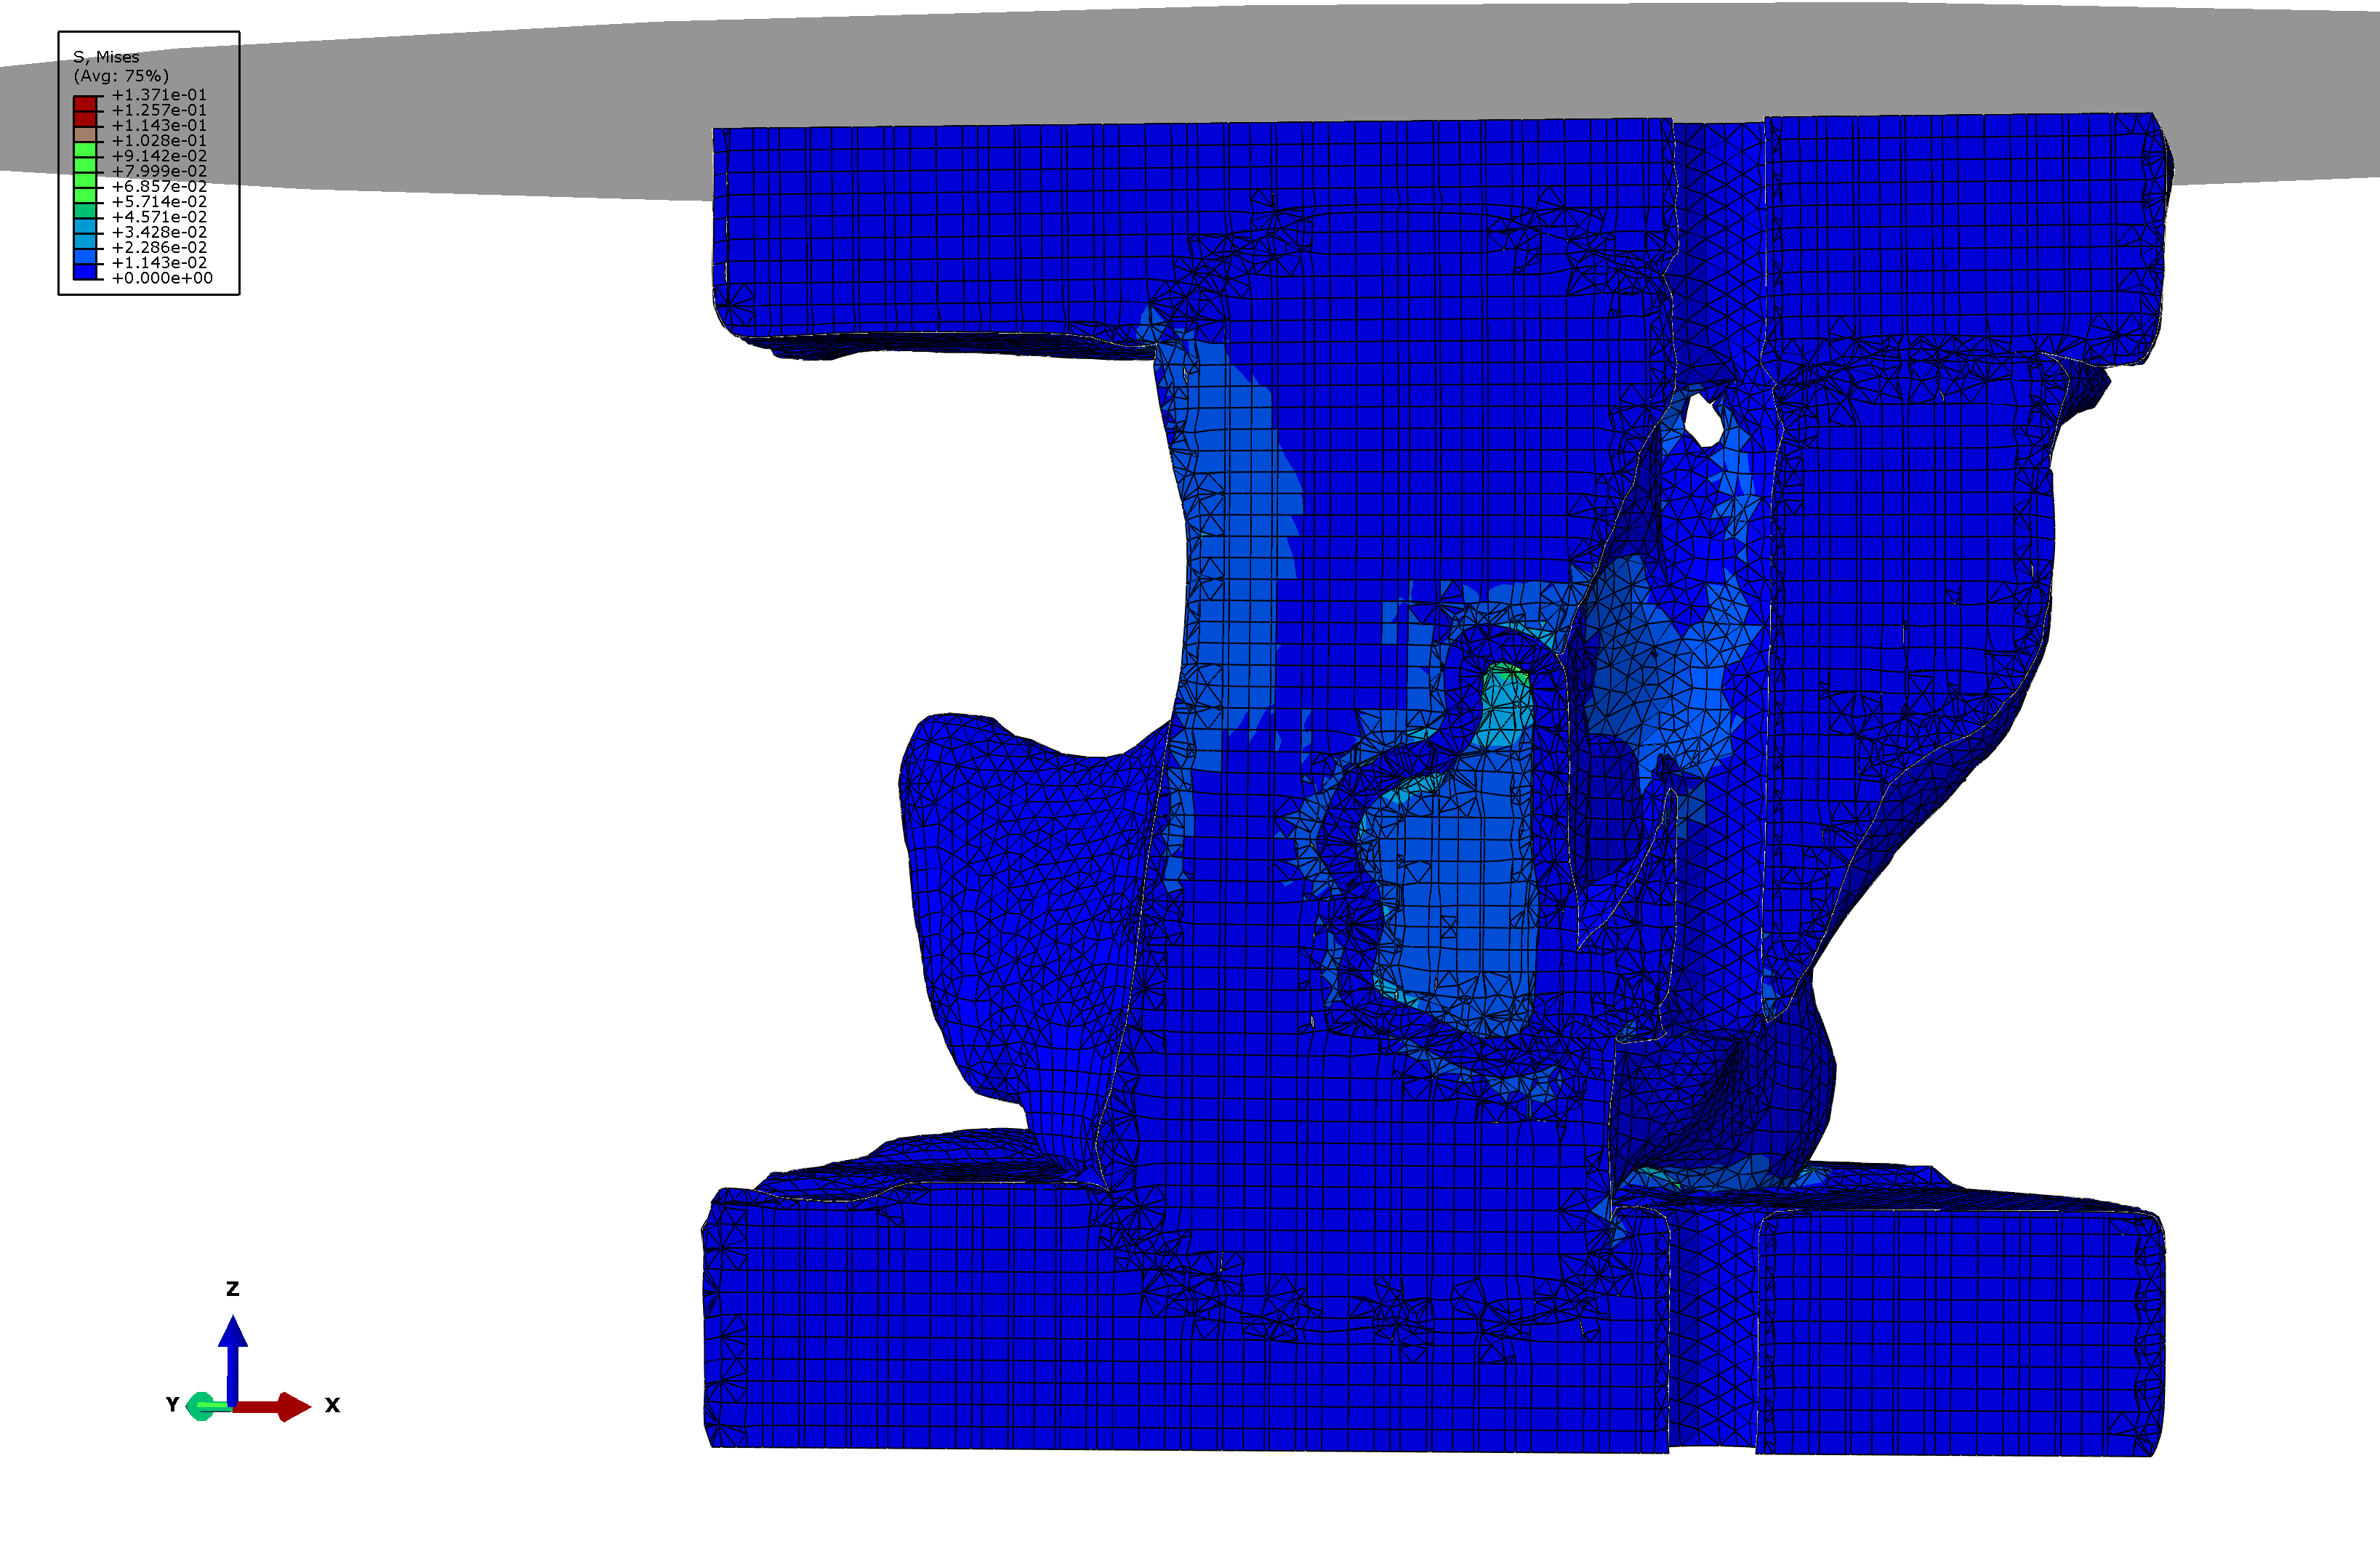
\includegraphics[width=10cm]{images/T8_CC2_postVP_Interface_ABAQUS_All_Side_Stress.png}   & 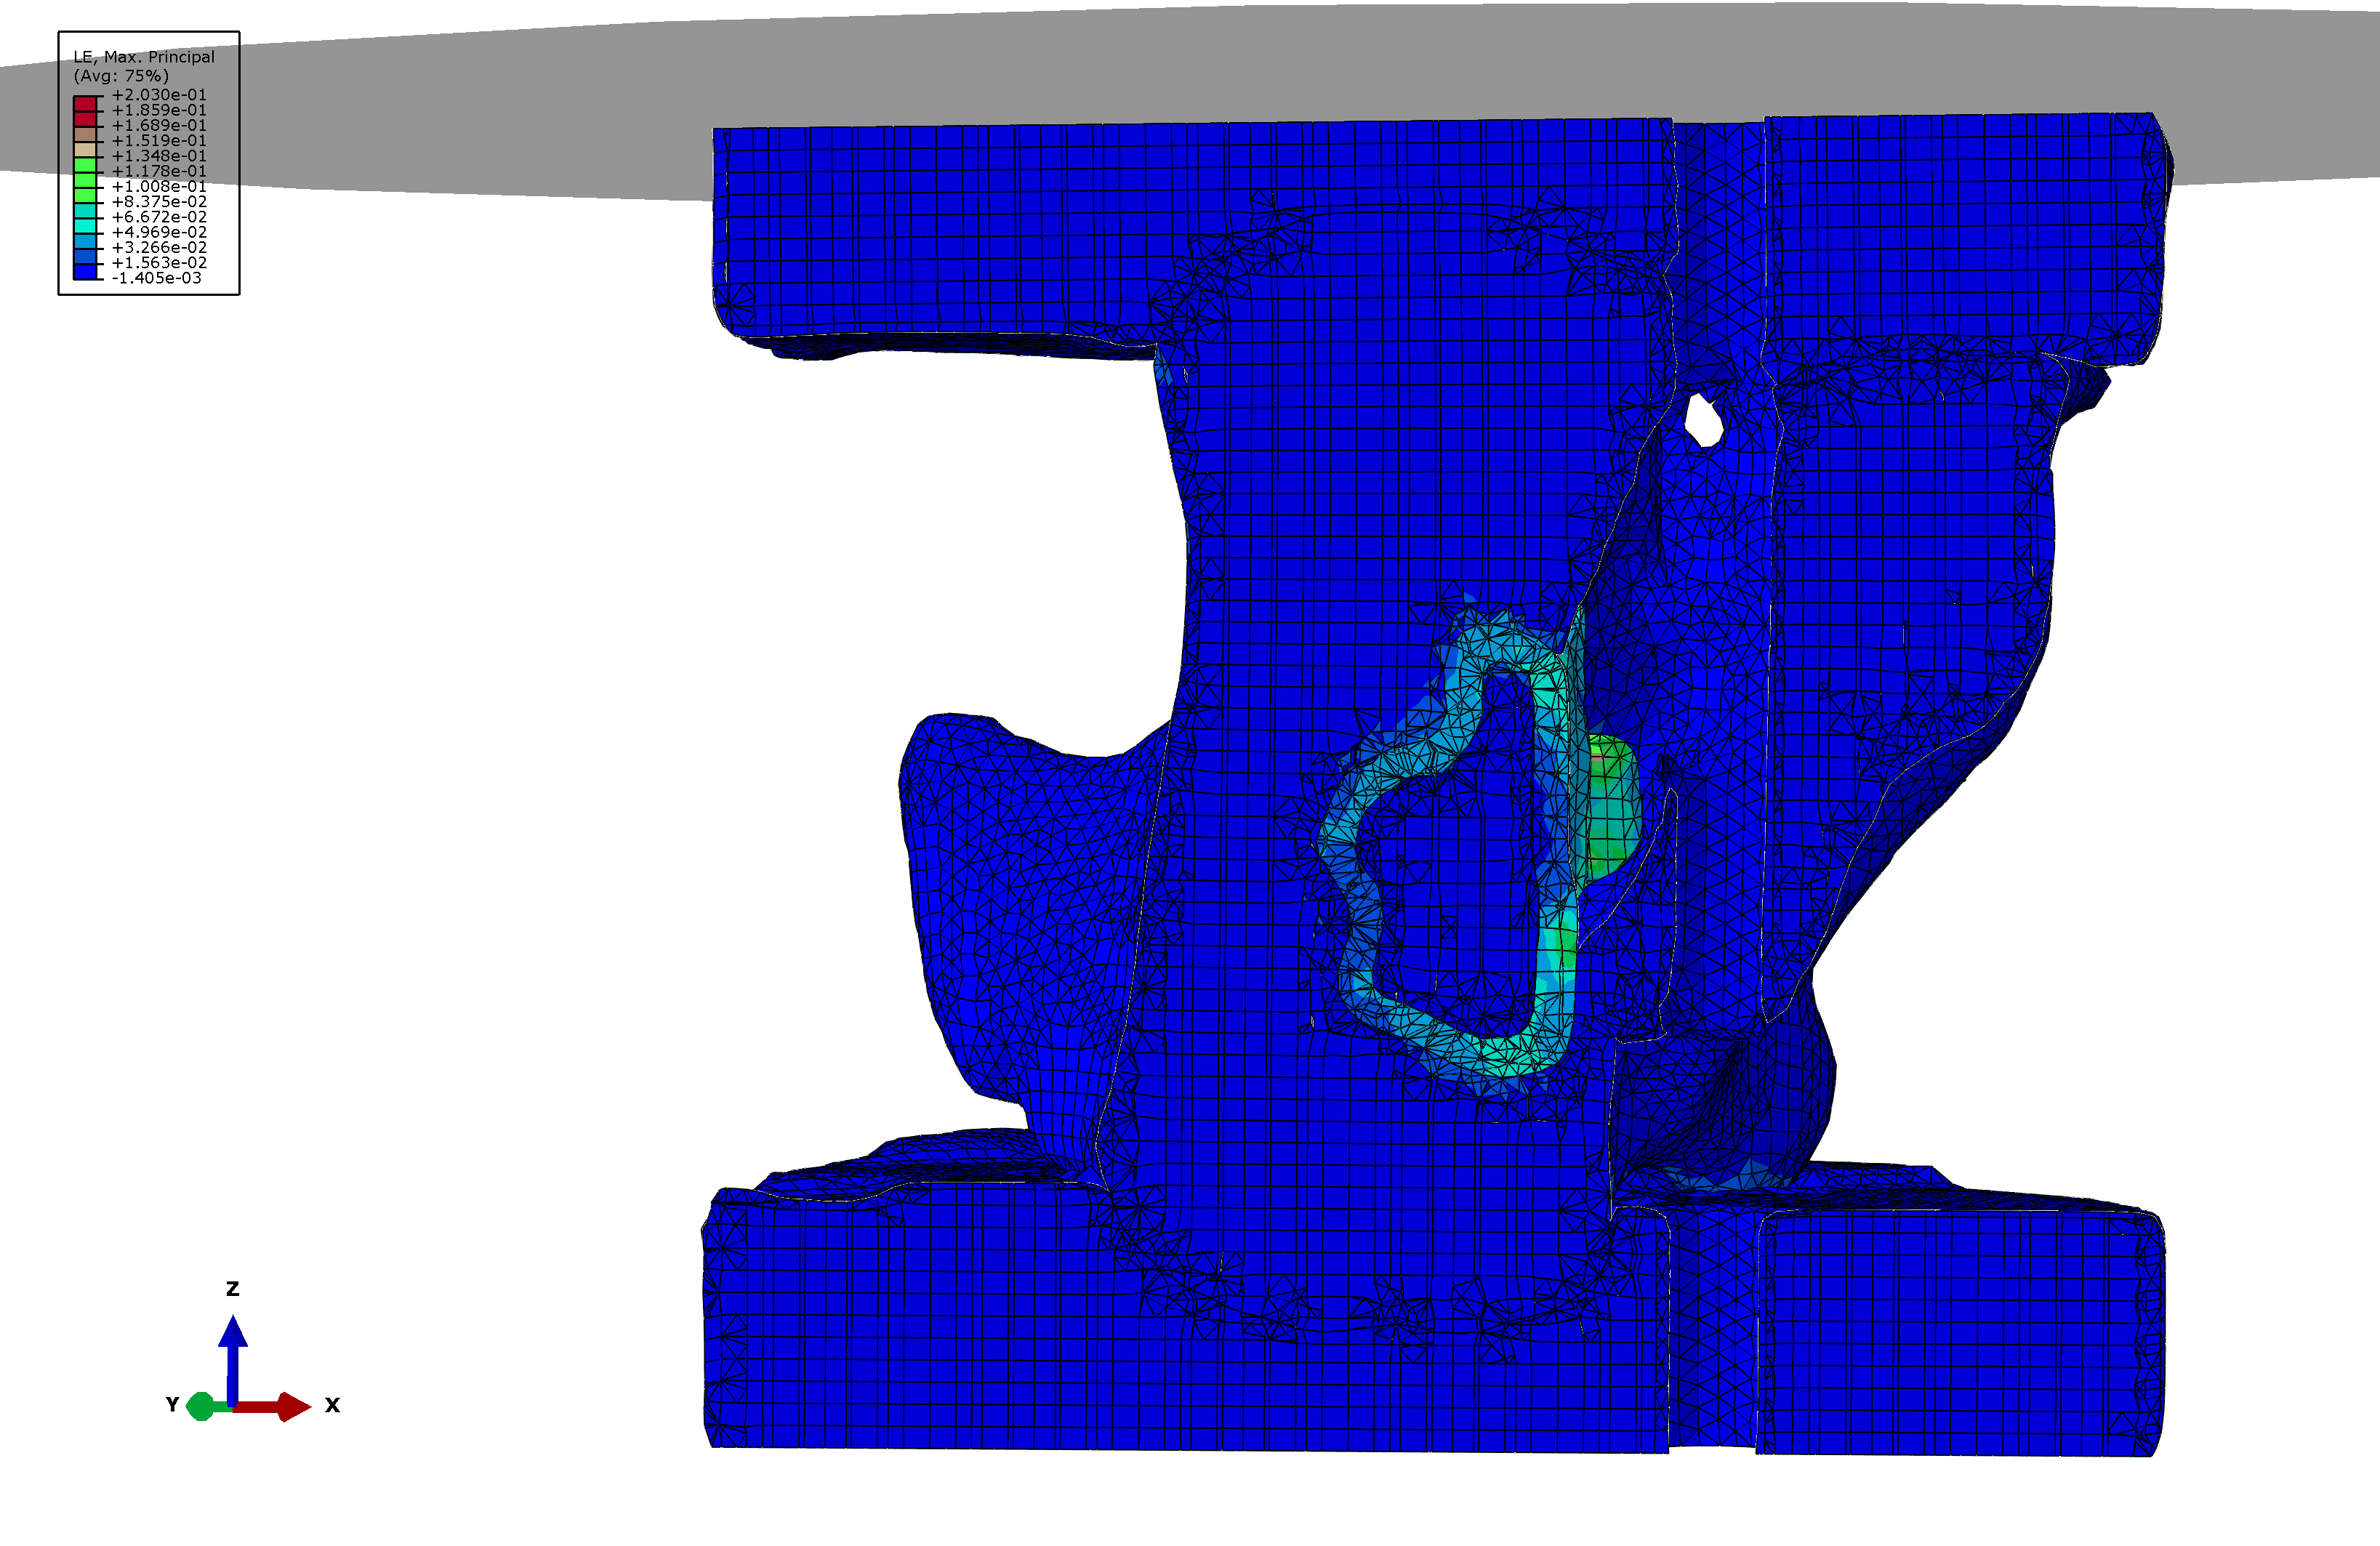
\includegraphics[width=10cm]{images/T8_CC2_postVP_Interface_ABAQUS_All_Side_Strain.png}   & T8 CC2  \begin{itemize} \item Experimental: 	7057.0	N/mm \item Computational:	3596.16 N/mm \item 13.3 \% Fill \end{itemize} \\ \hline 
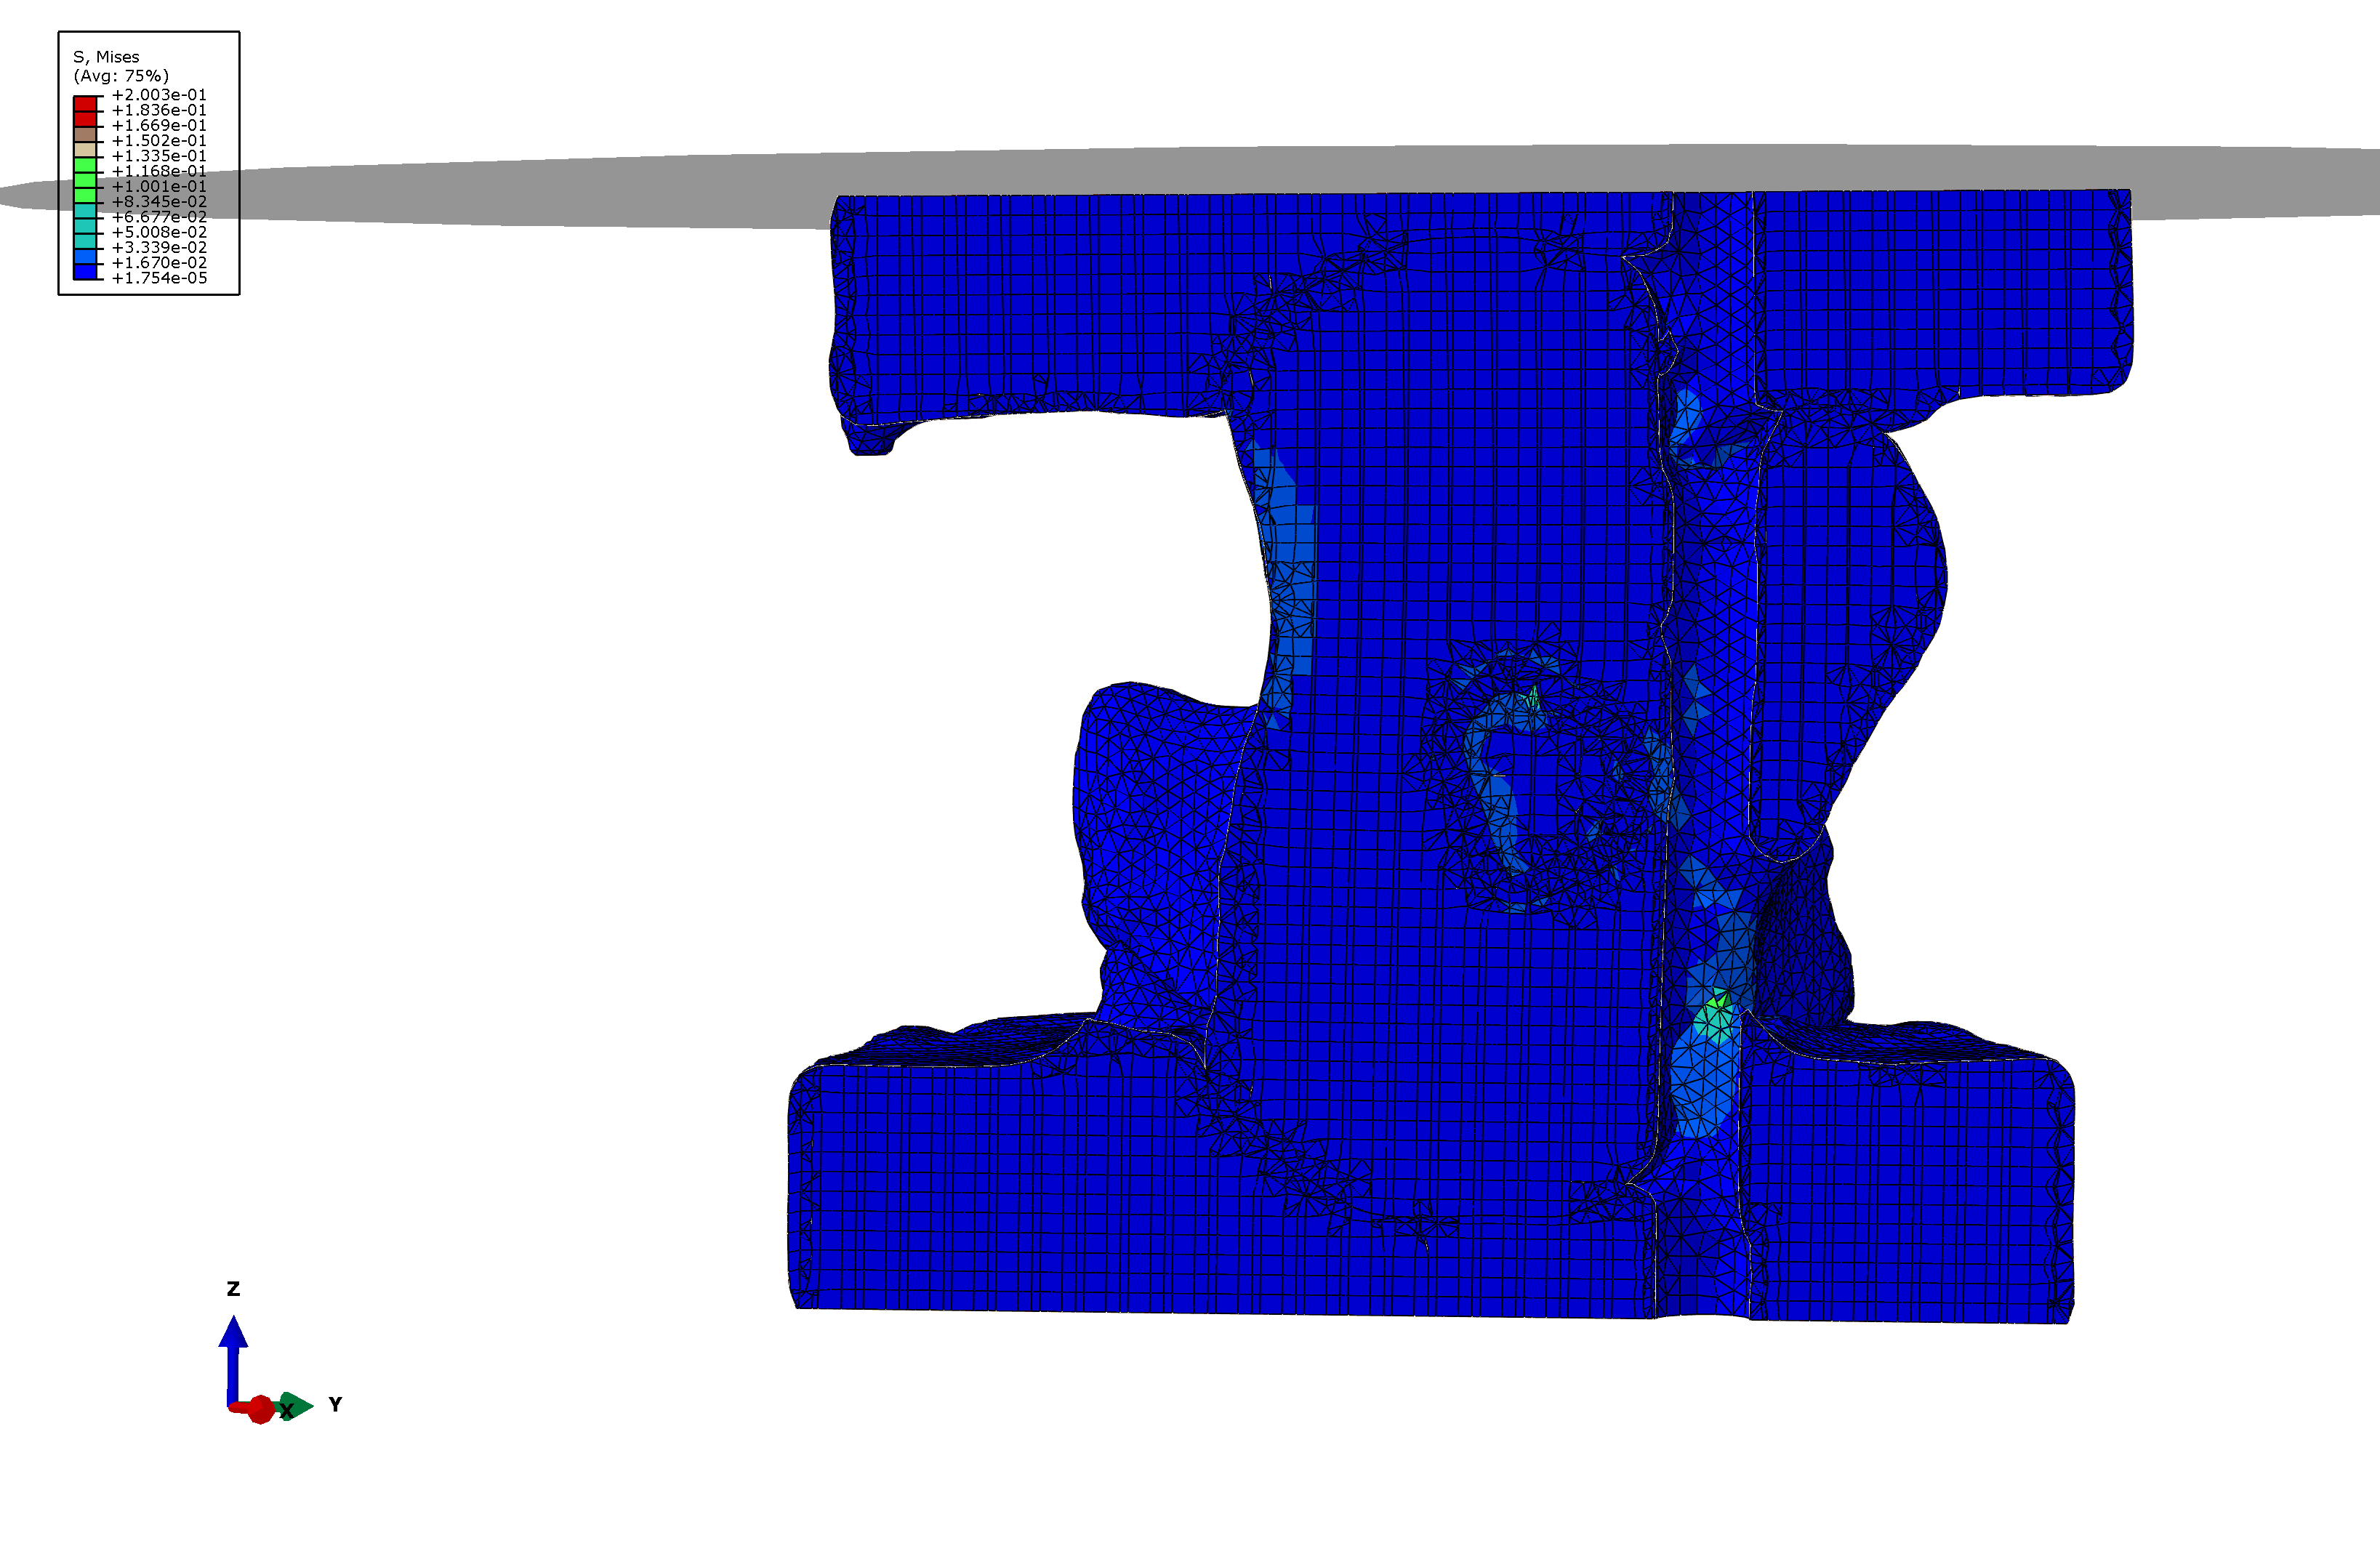
\includegraphics[width=10cm]{images/T8_CC3_postVP_Interface_ABAQUS_All_Side_Stress.png}   & 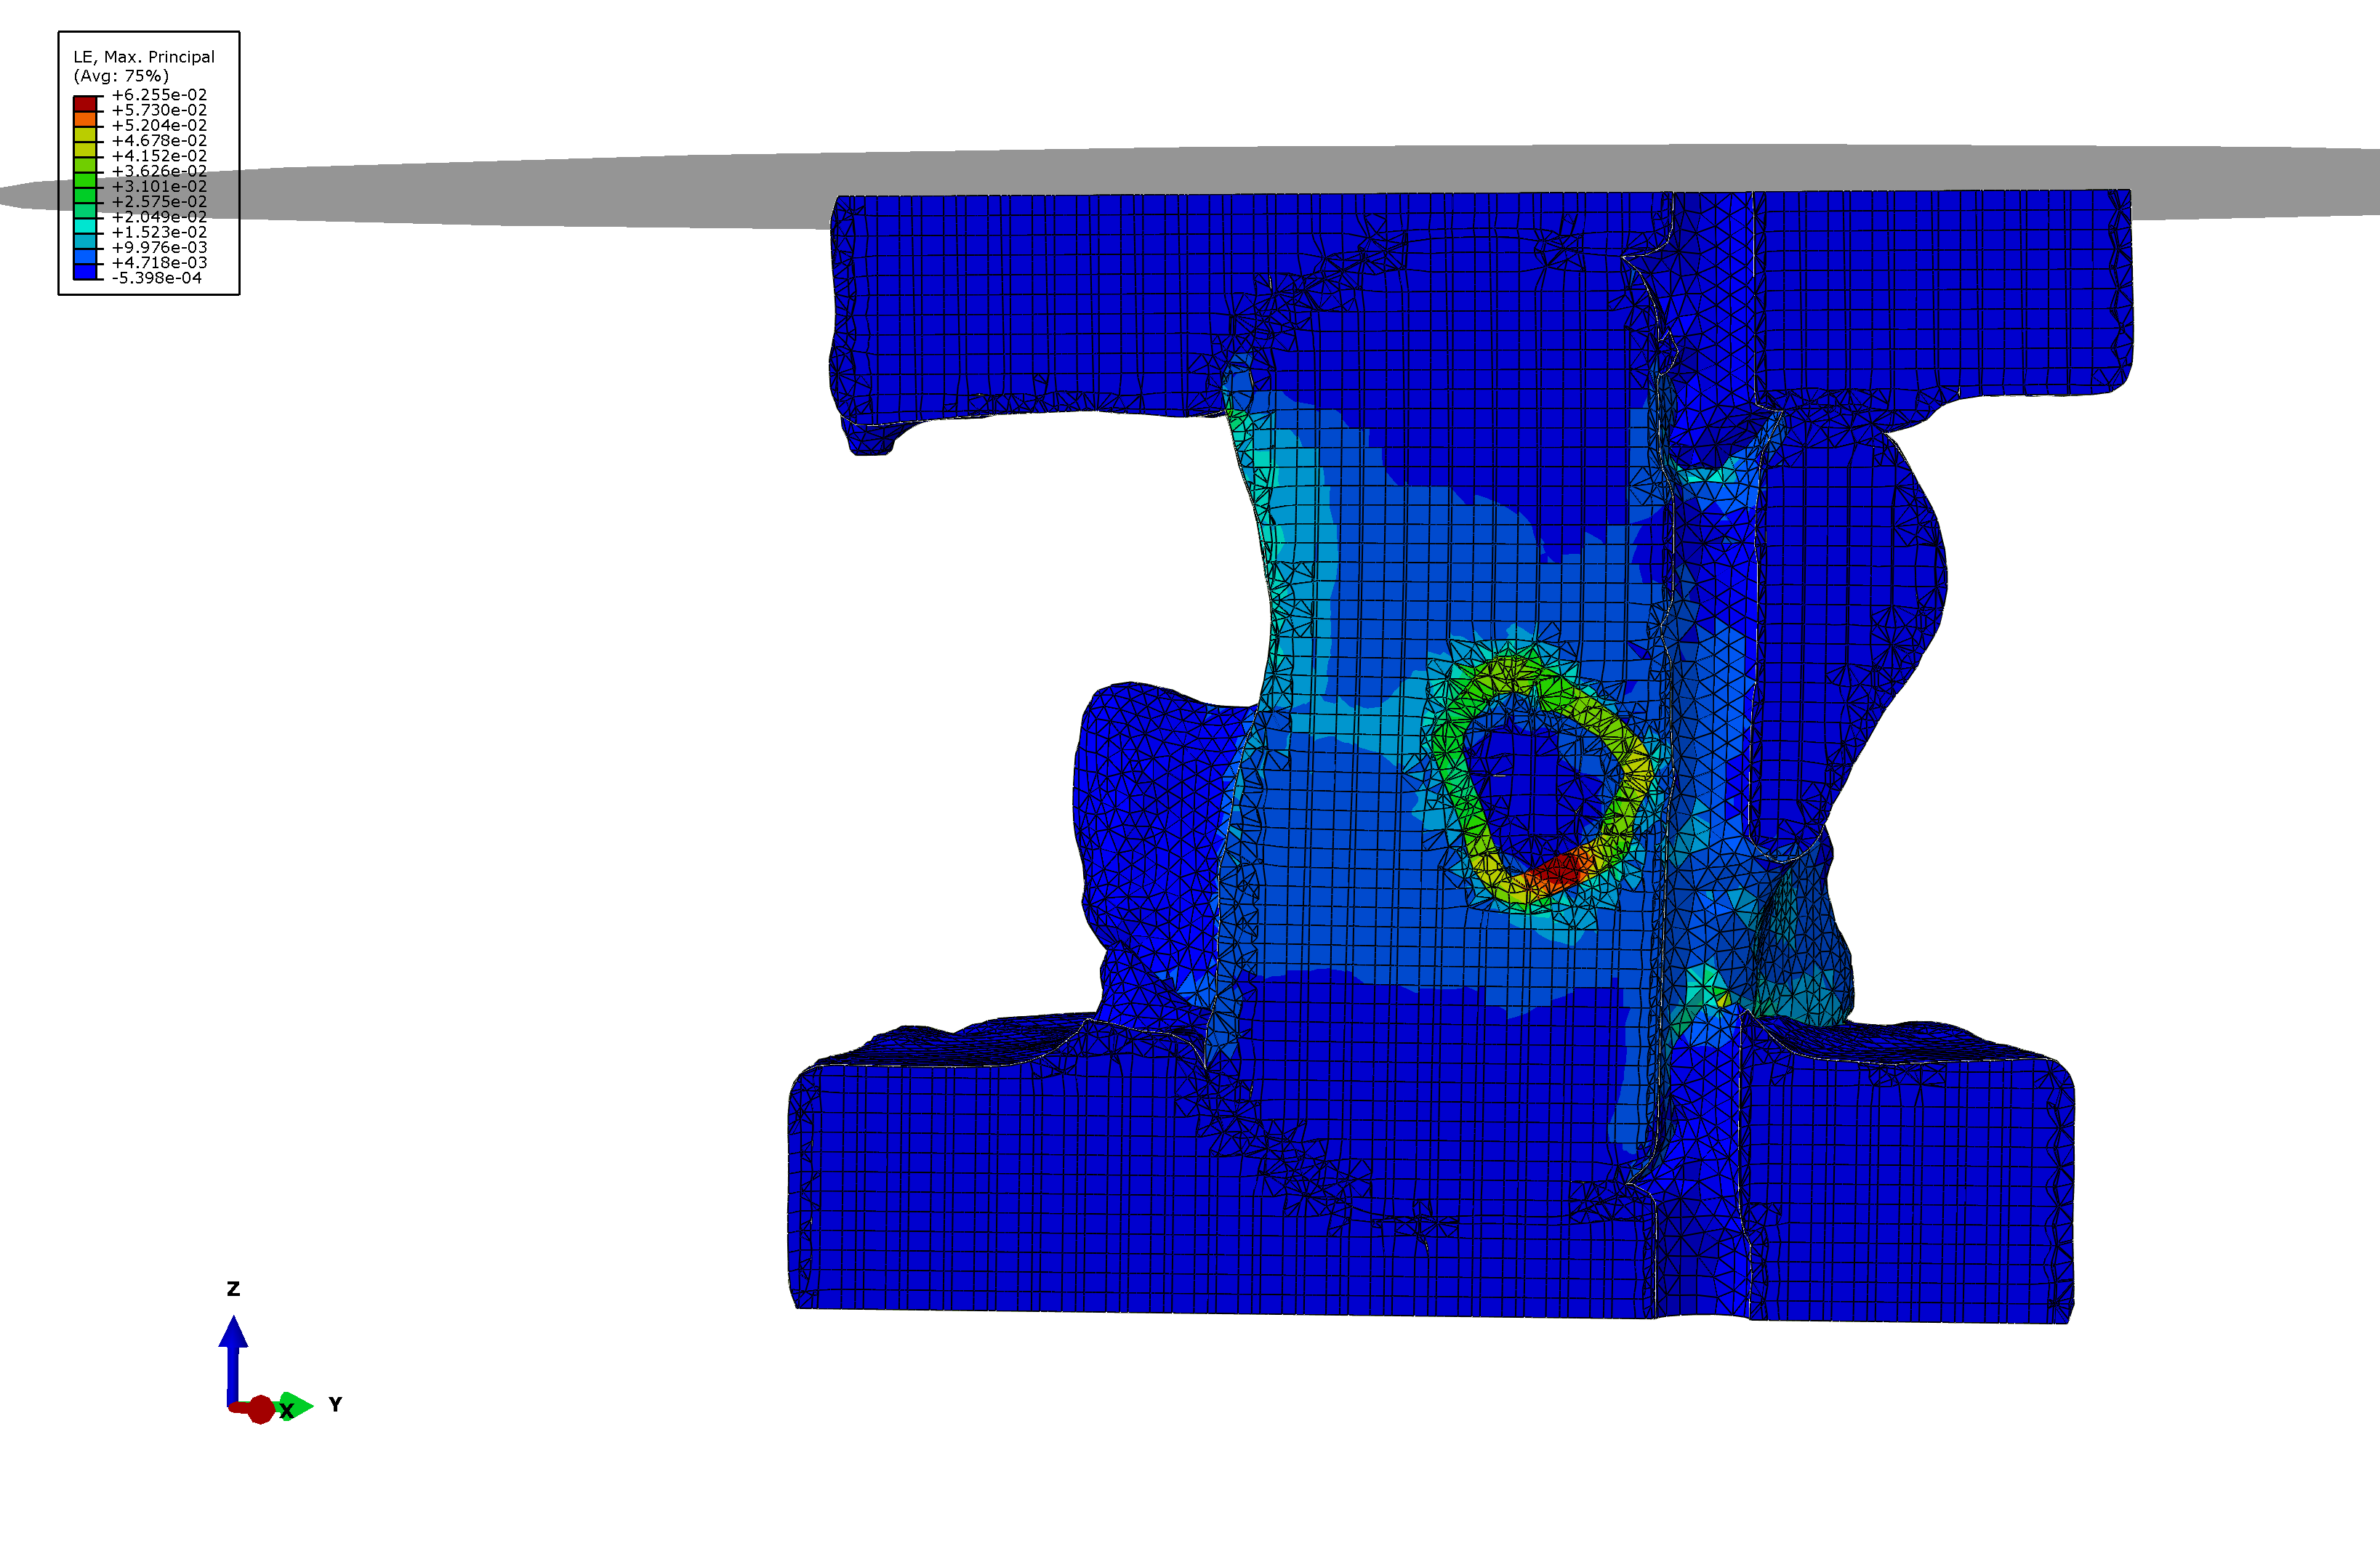
\includegraphics[width=10cm]{images/T8_CC3_postVP_Interface_ABAQUS_All_Side_Strain.png}   & T8 CC3  \begin{itemize} \item Experimental: 	5873.1	N/mm \item Computational:	4713.04 N/mm \item 3.4 \% Fill \end{itemize} \\ \hline 
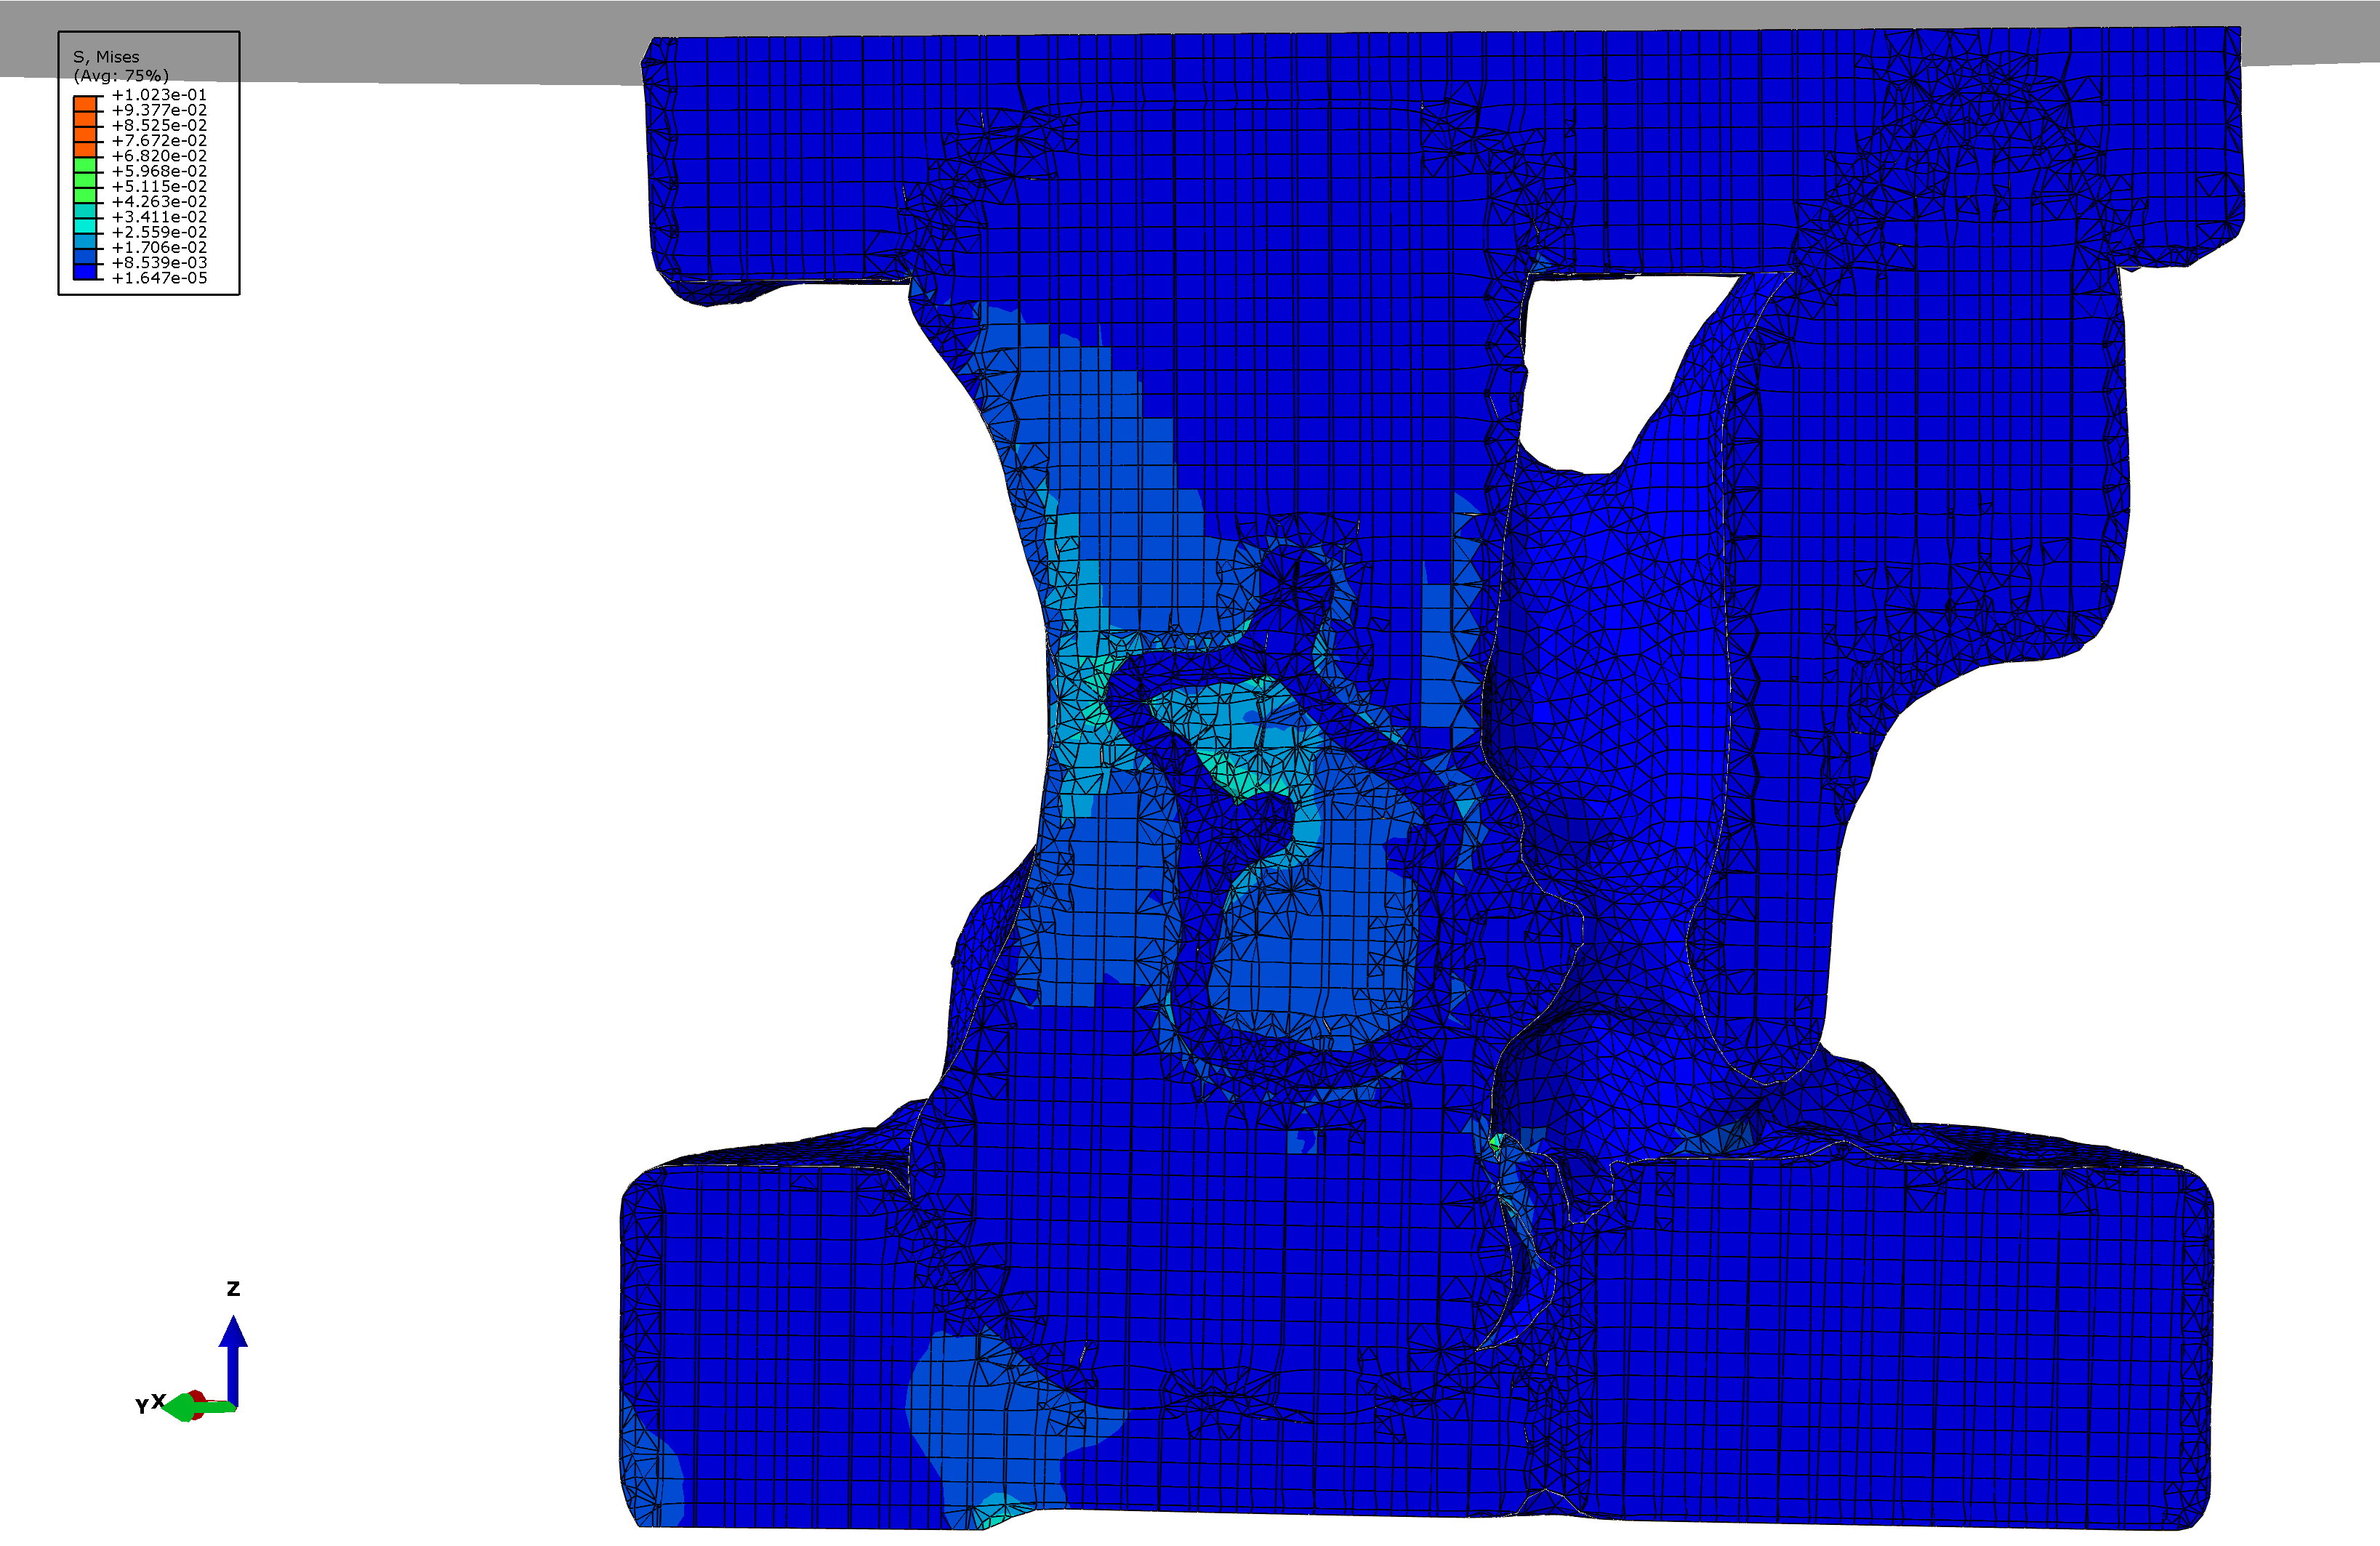
\includegraphics[width=10cm]{images/T9_CC1_postVP_Interface_ABAQUS_All_Side_Stress.png}   & 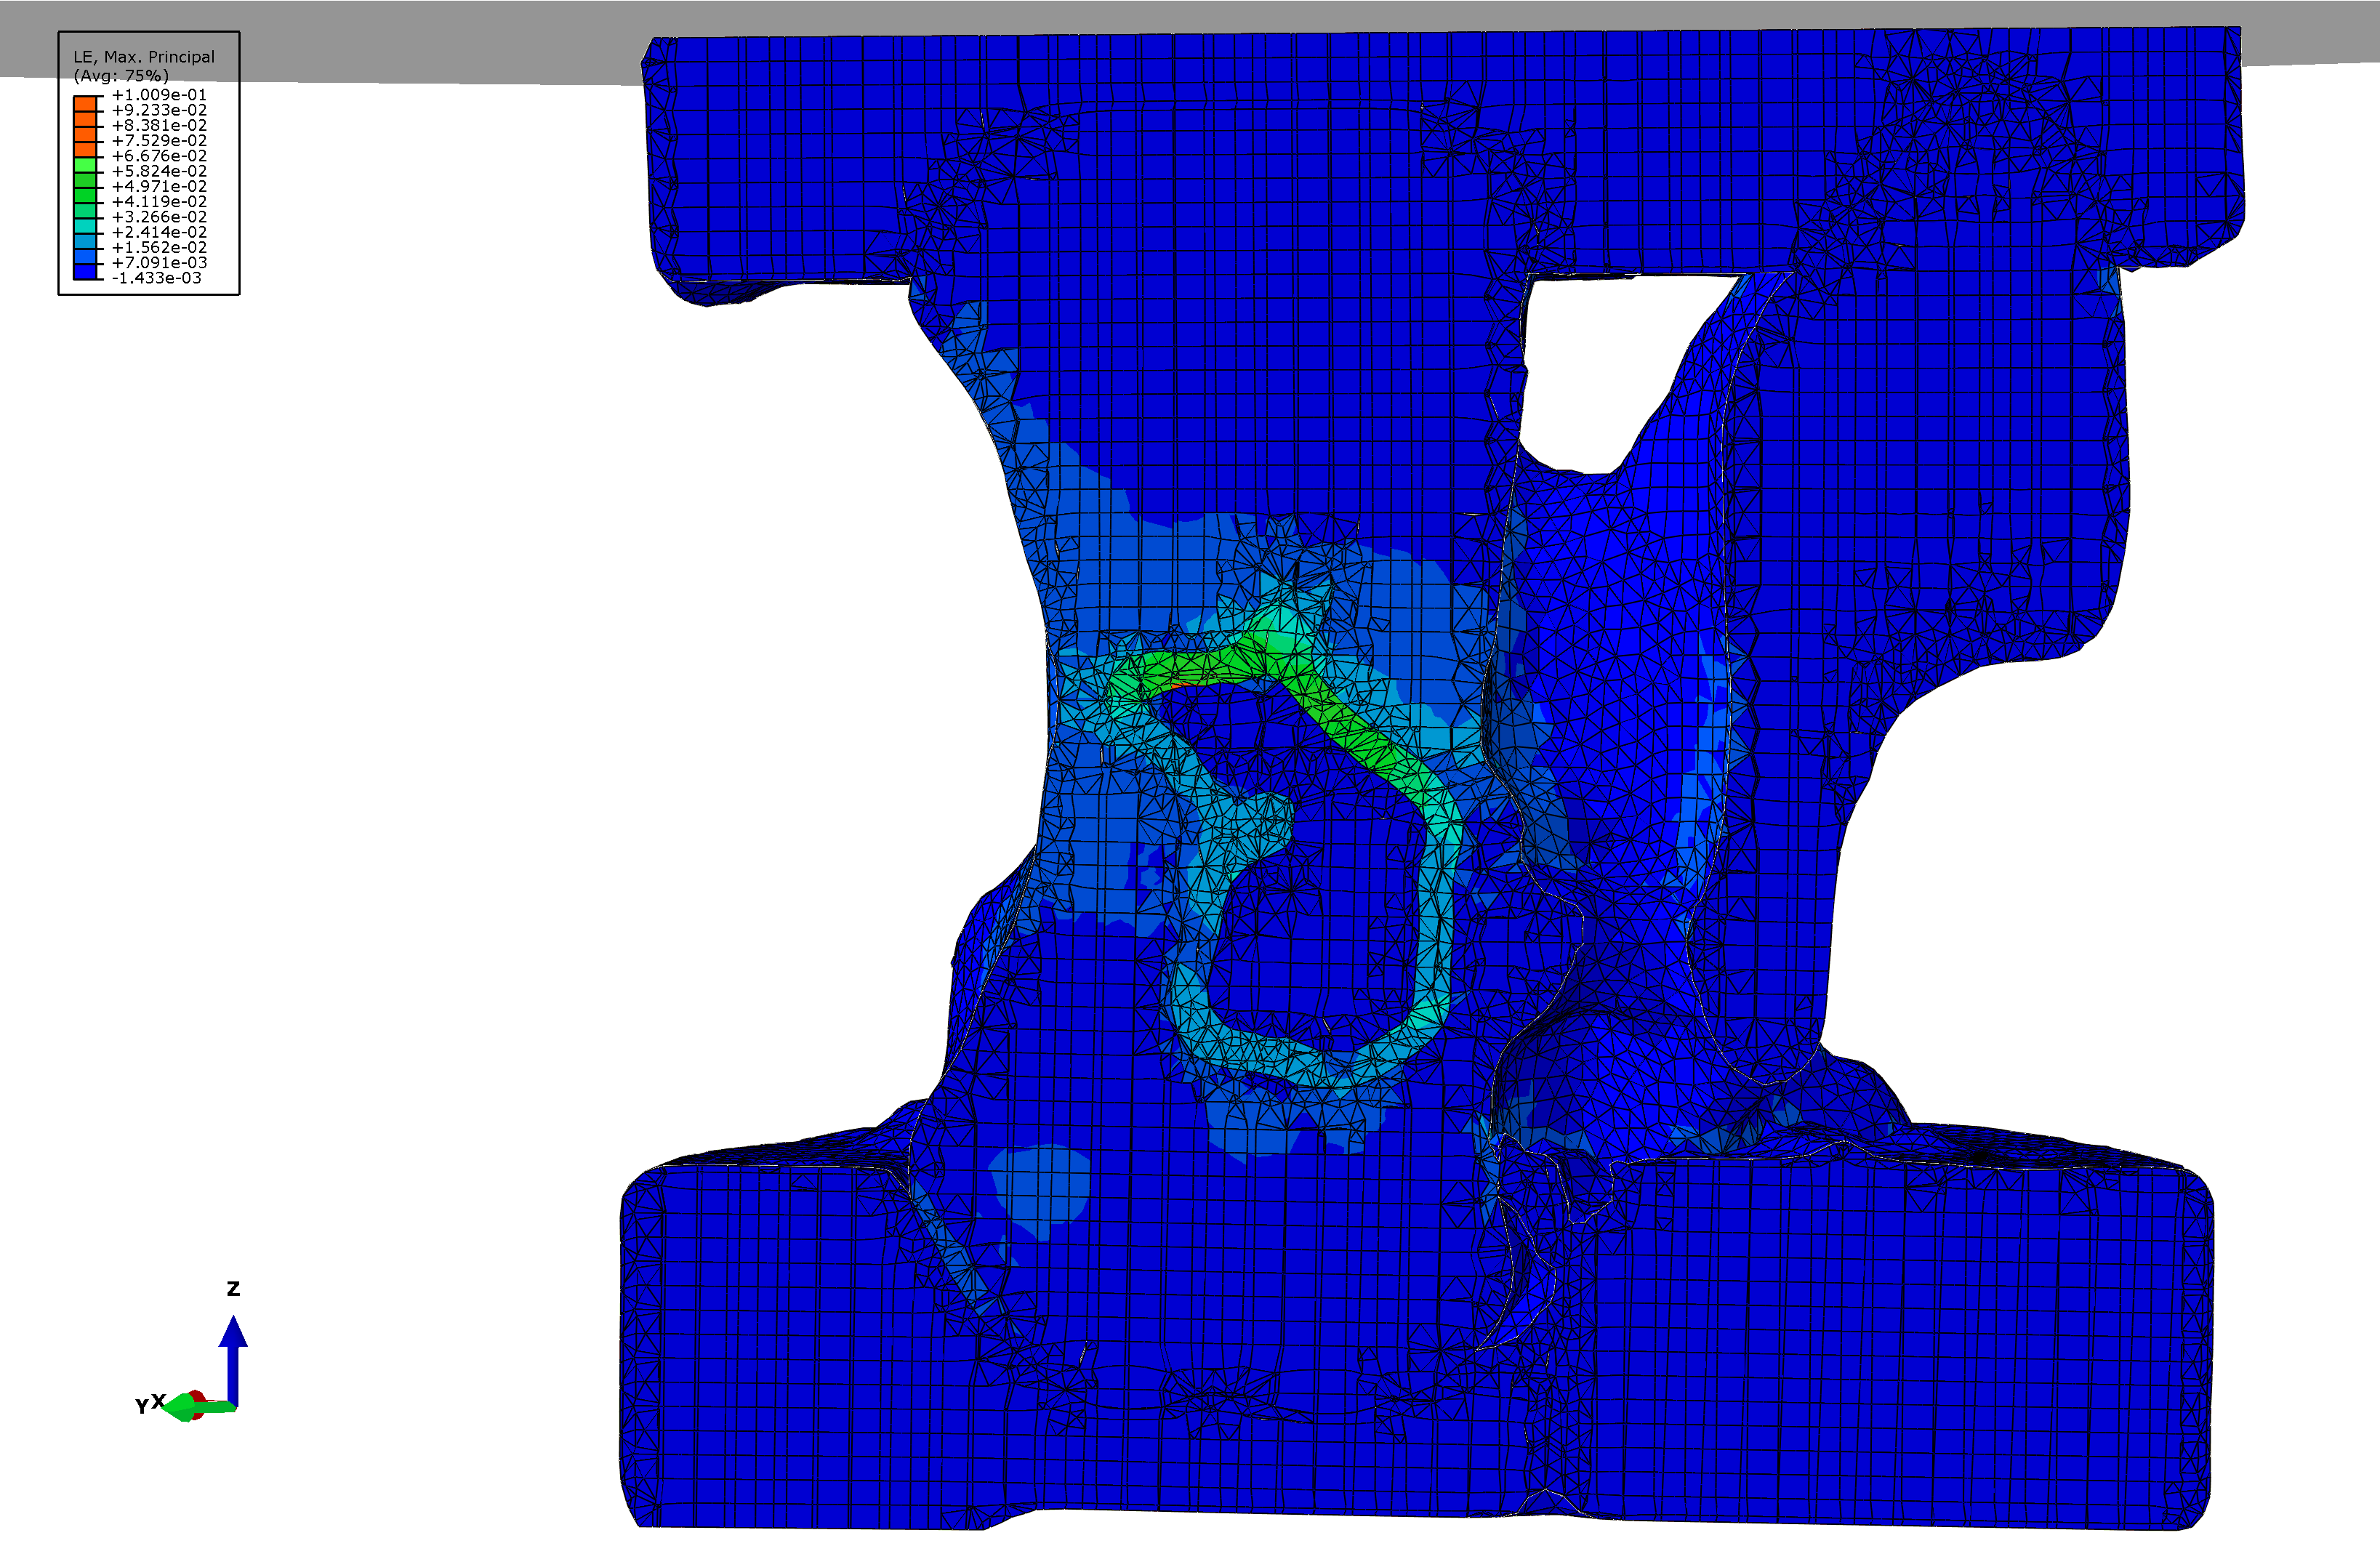
\includegraphics[width=10cm]{images/T9_CC1_postVP_Interface_ABAQUS_All_Side_Strain.png}   & T9 CC1  \begin{itemize} \item Experimental: 	4255.4	N/mm \item Computational:	4318.79 N/mm \item 6.0 \% Fill \end{itemize} \\ \hline 
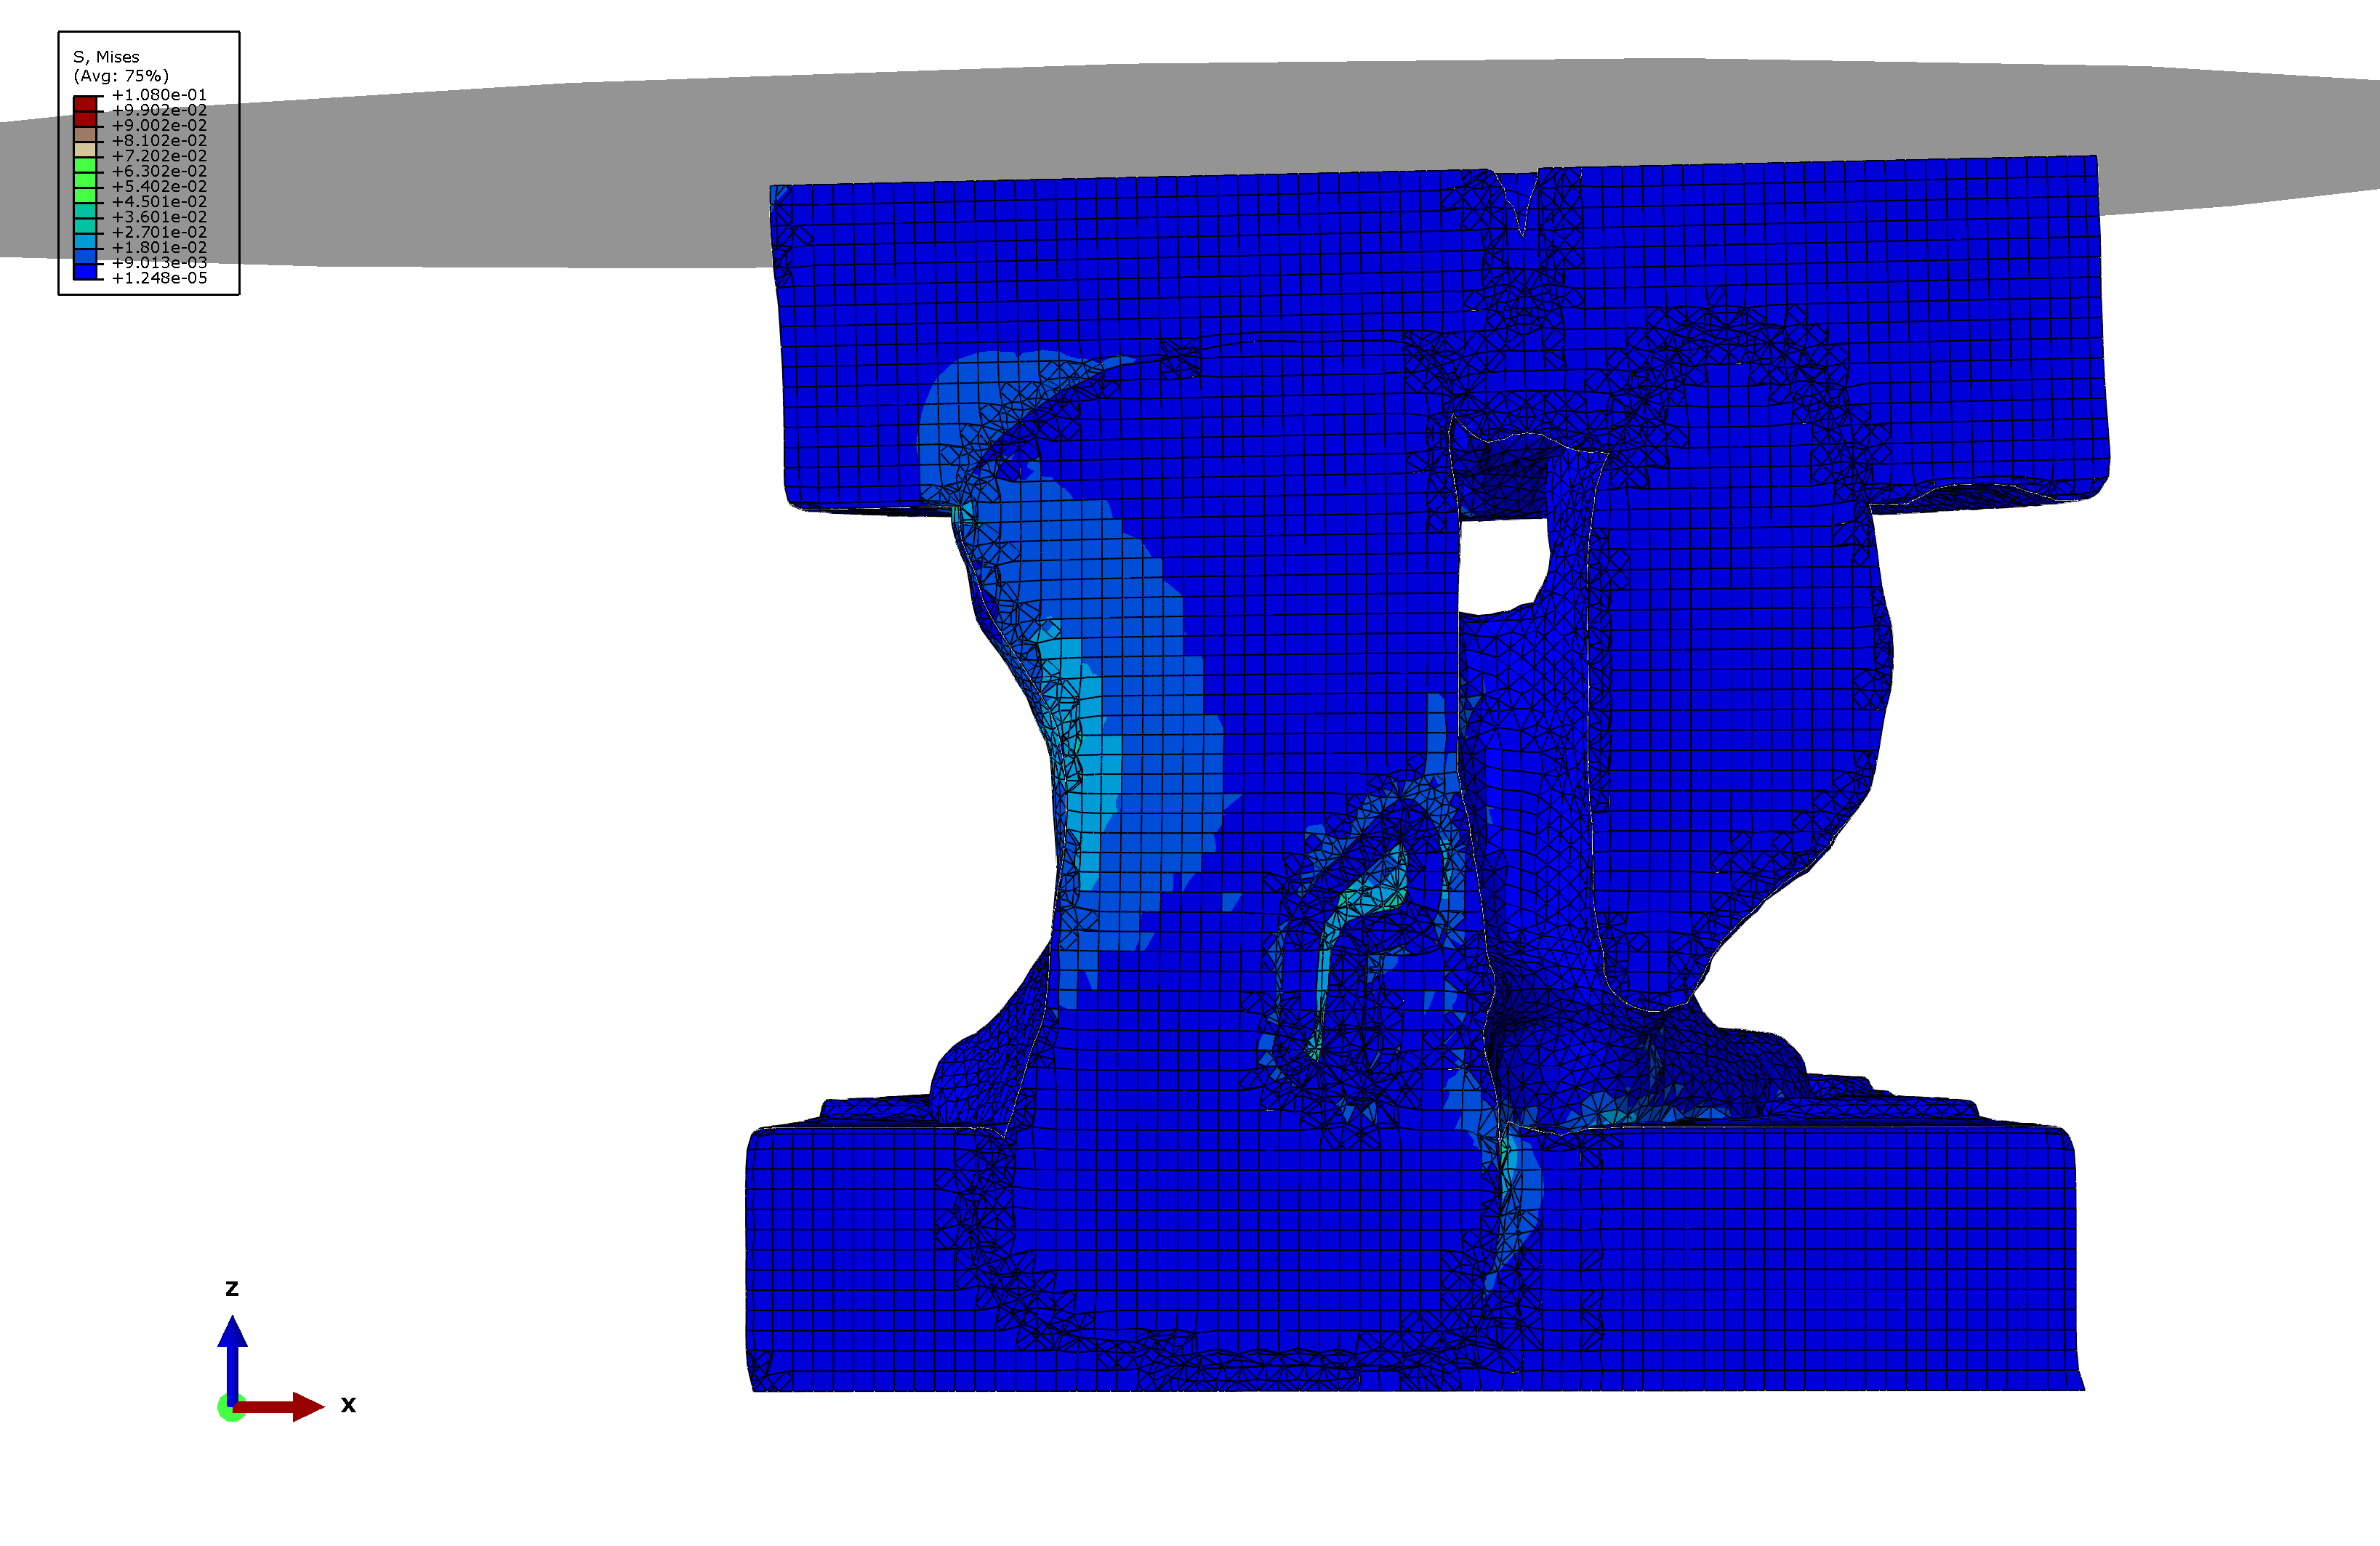
\includegraphics[width=10cm]{images/T9_CC2_postVP_Interface_ABAQUS_All_Side_Stress.png}   & 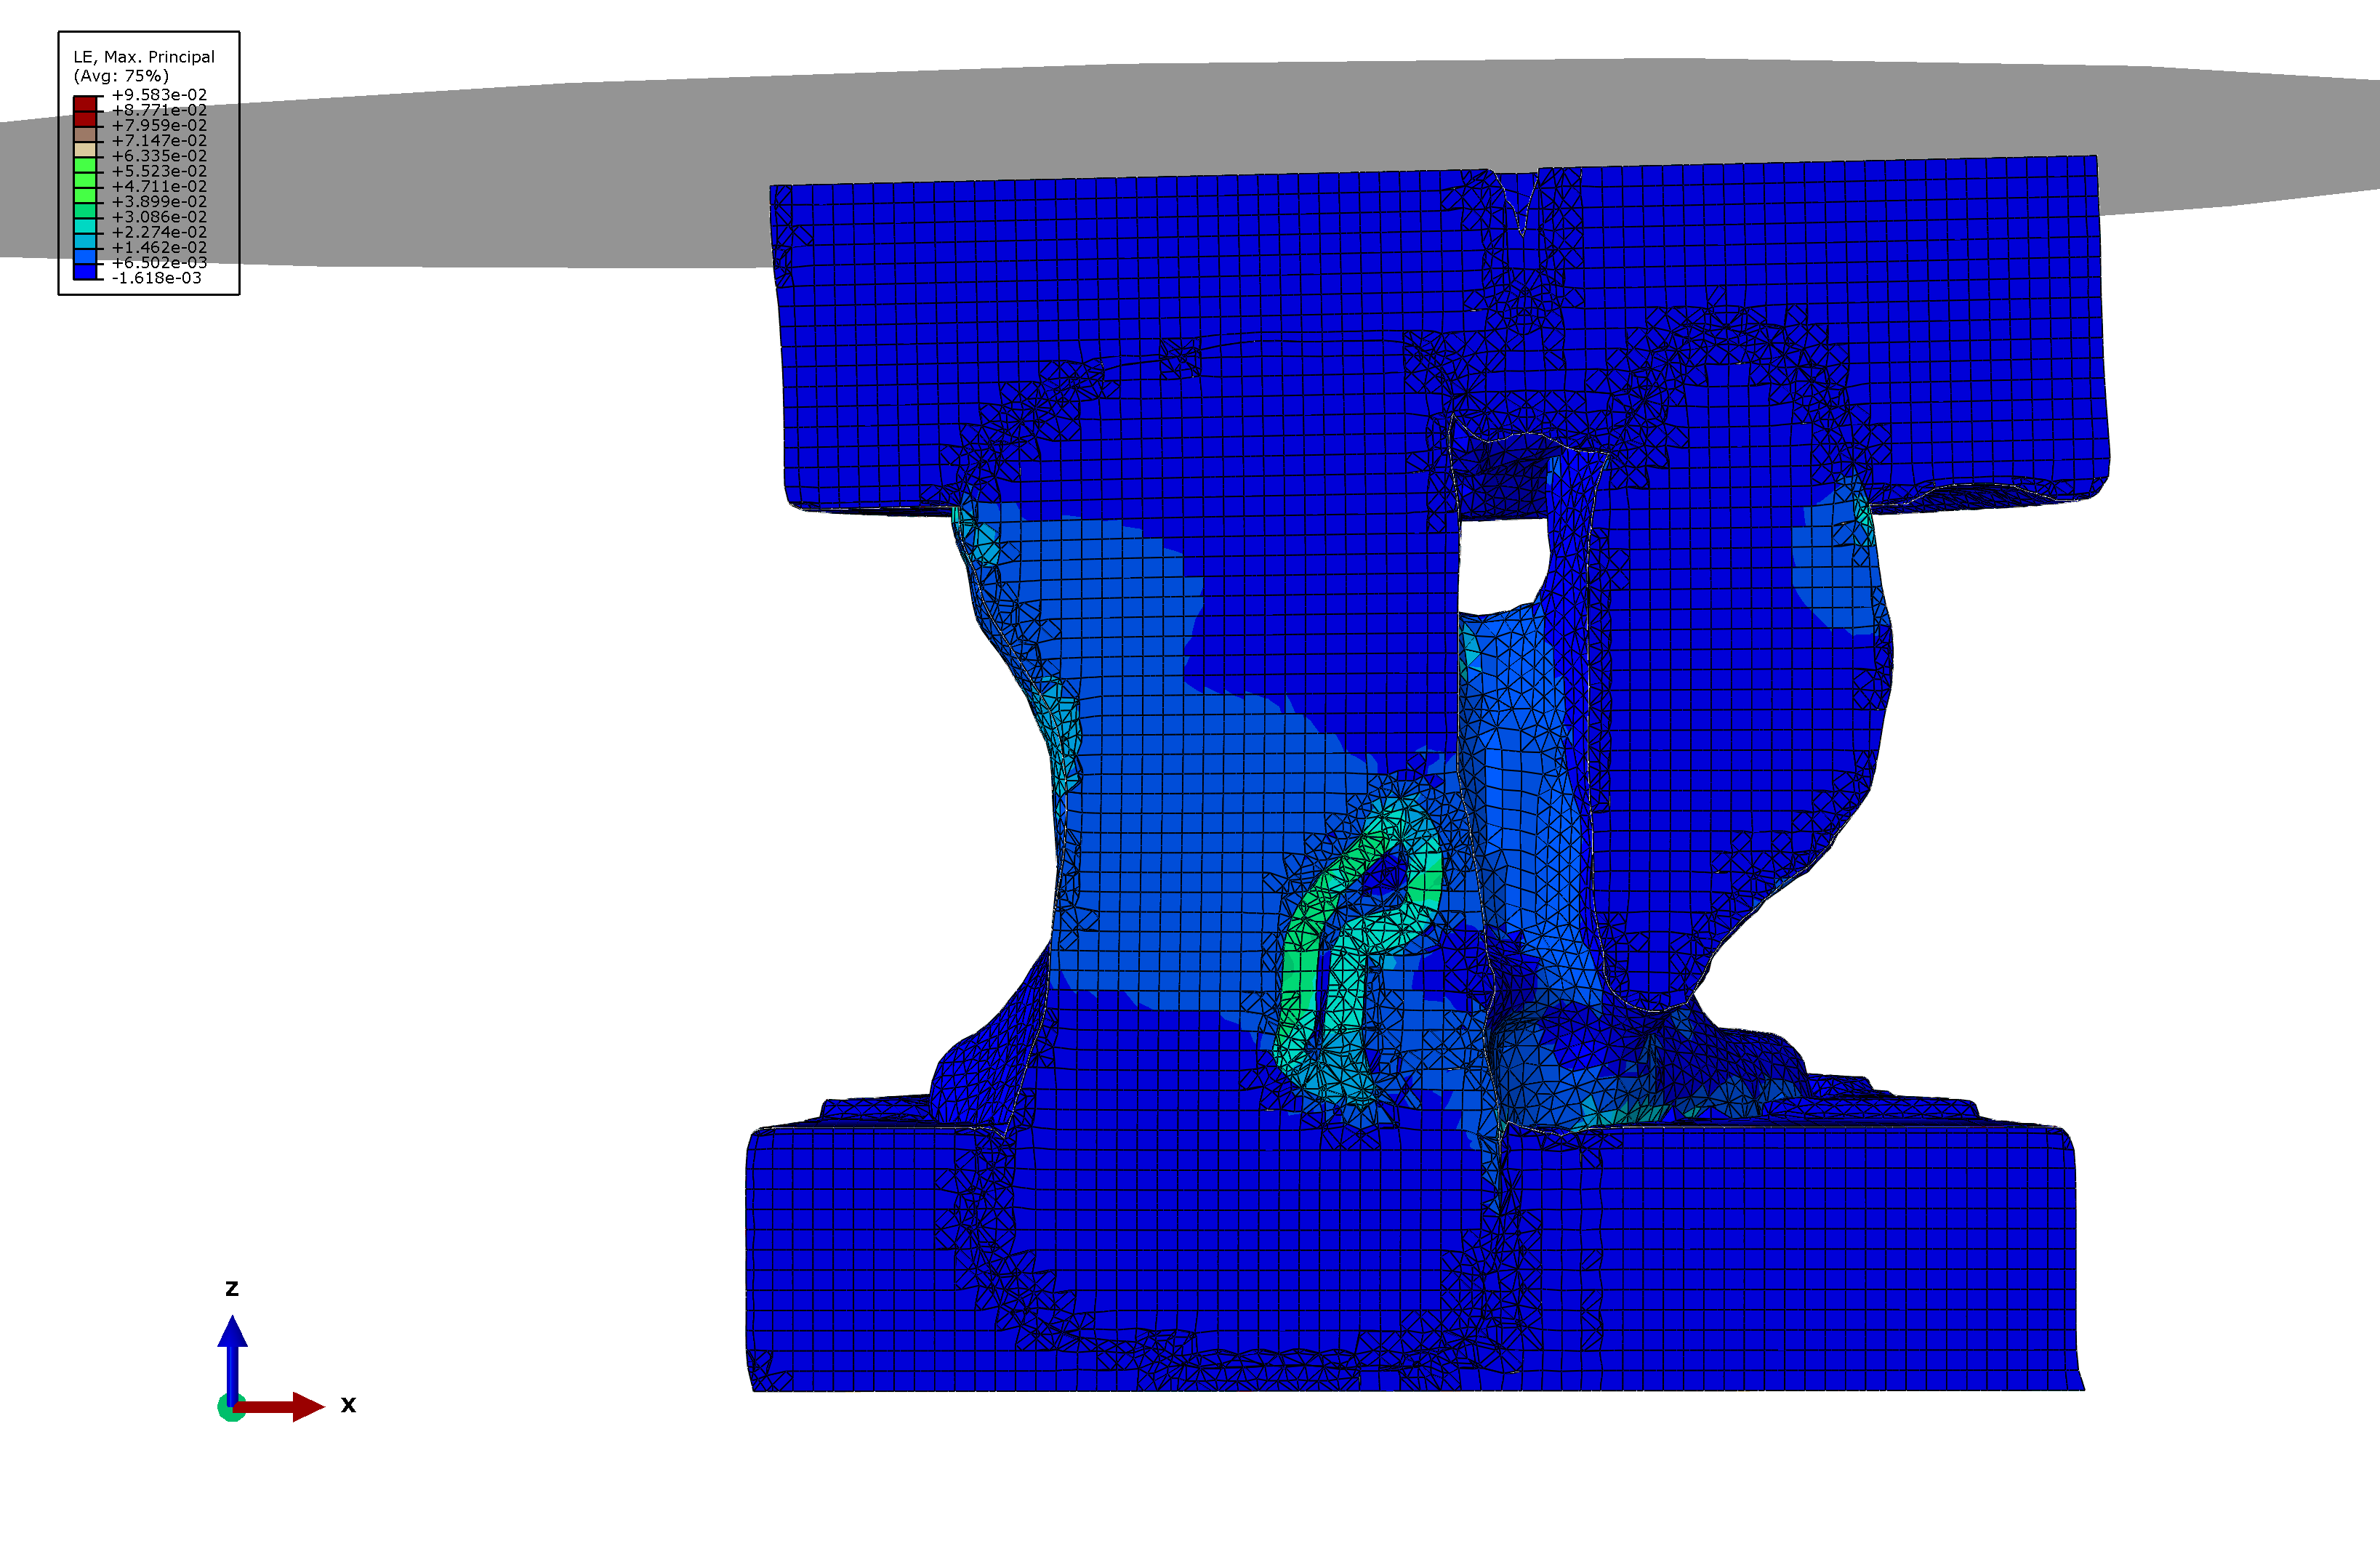
\includegraphics[width=10cm]{images/T9_CC2_postVP_Interface_ABAQUS_All_Side_Strain.png}   & T9 CC2  \begin{itemize} \item Experimental: 	3654.3	N/mm \item Computational:	4844.32 N/mm \item 5.1 \% Fill \end{itemize} \\ \hline 
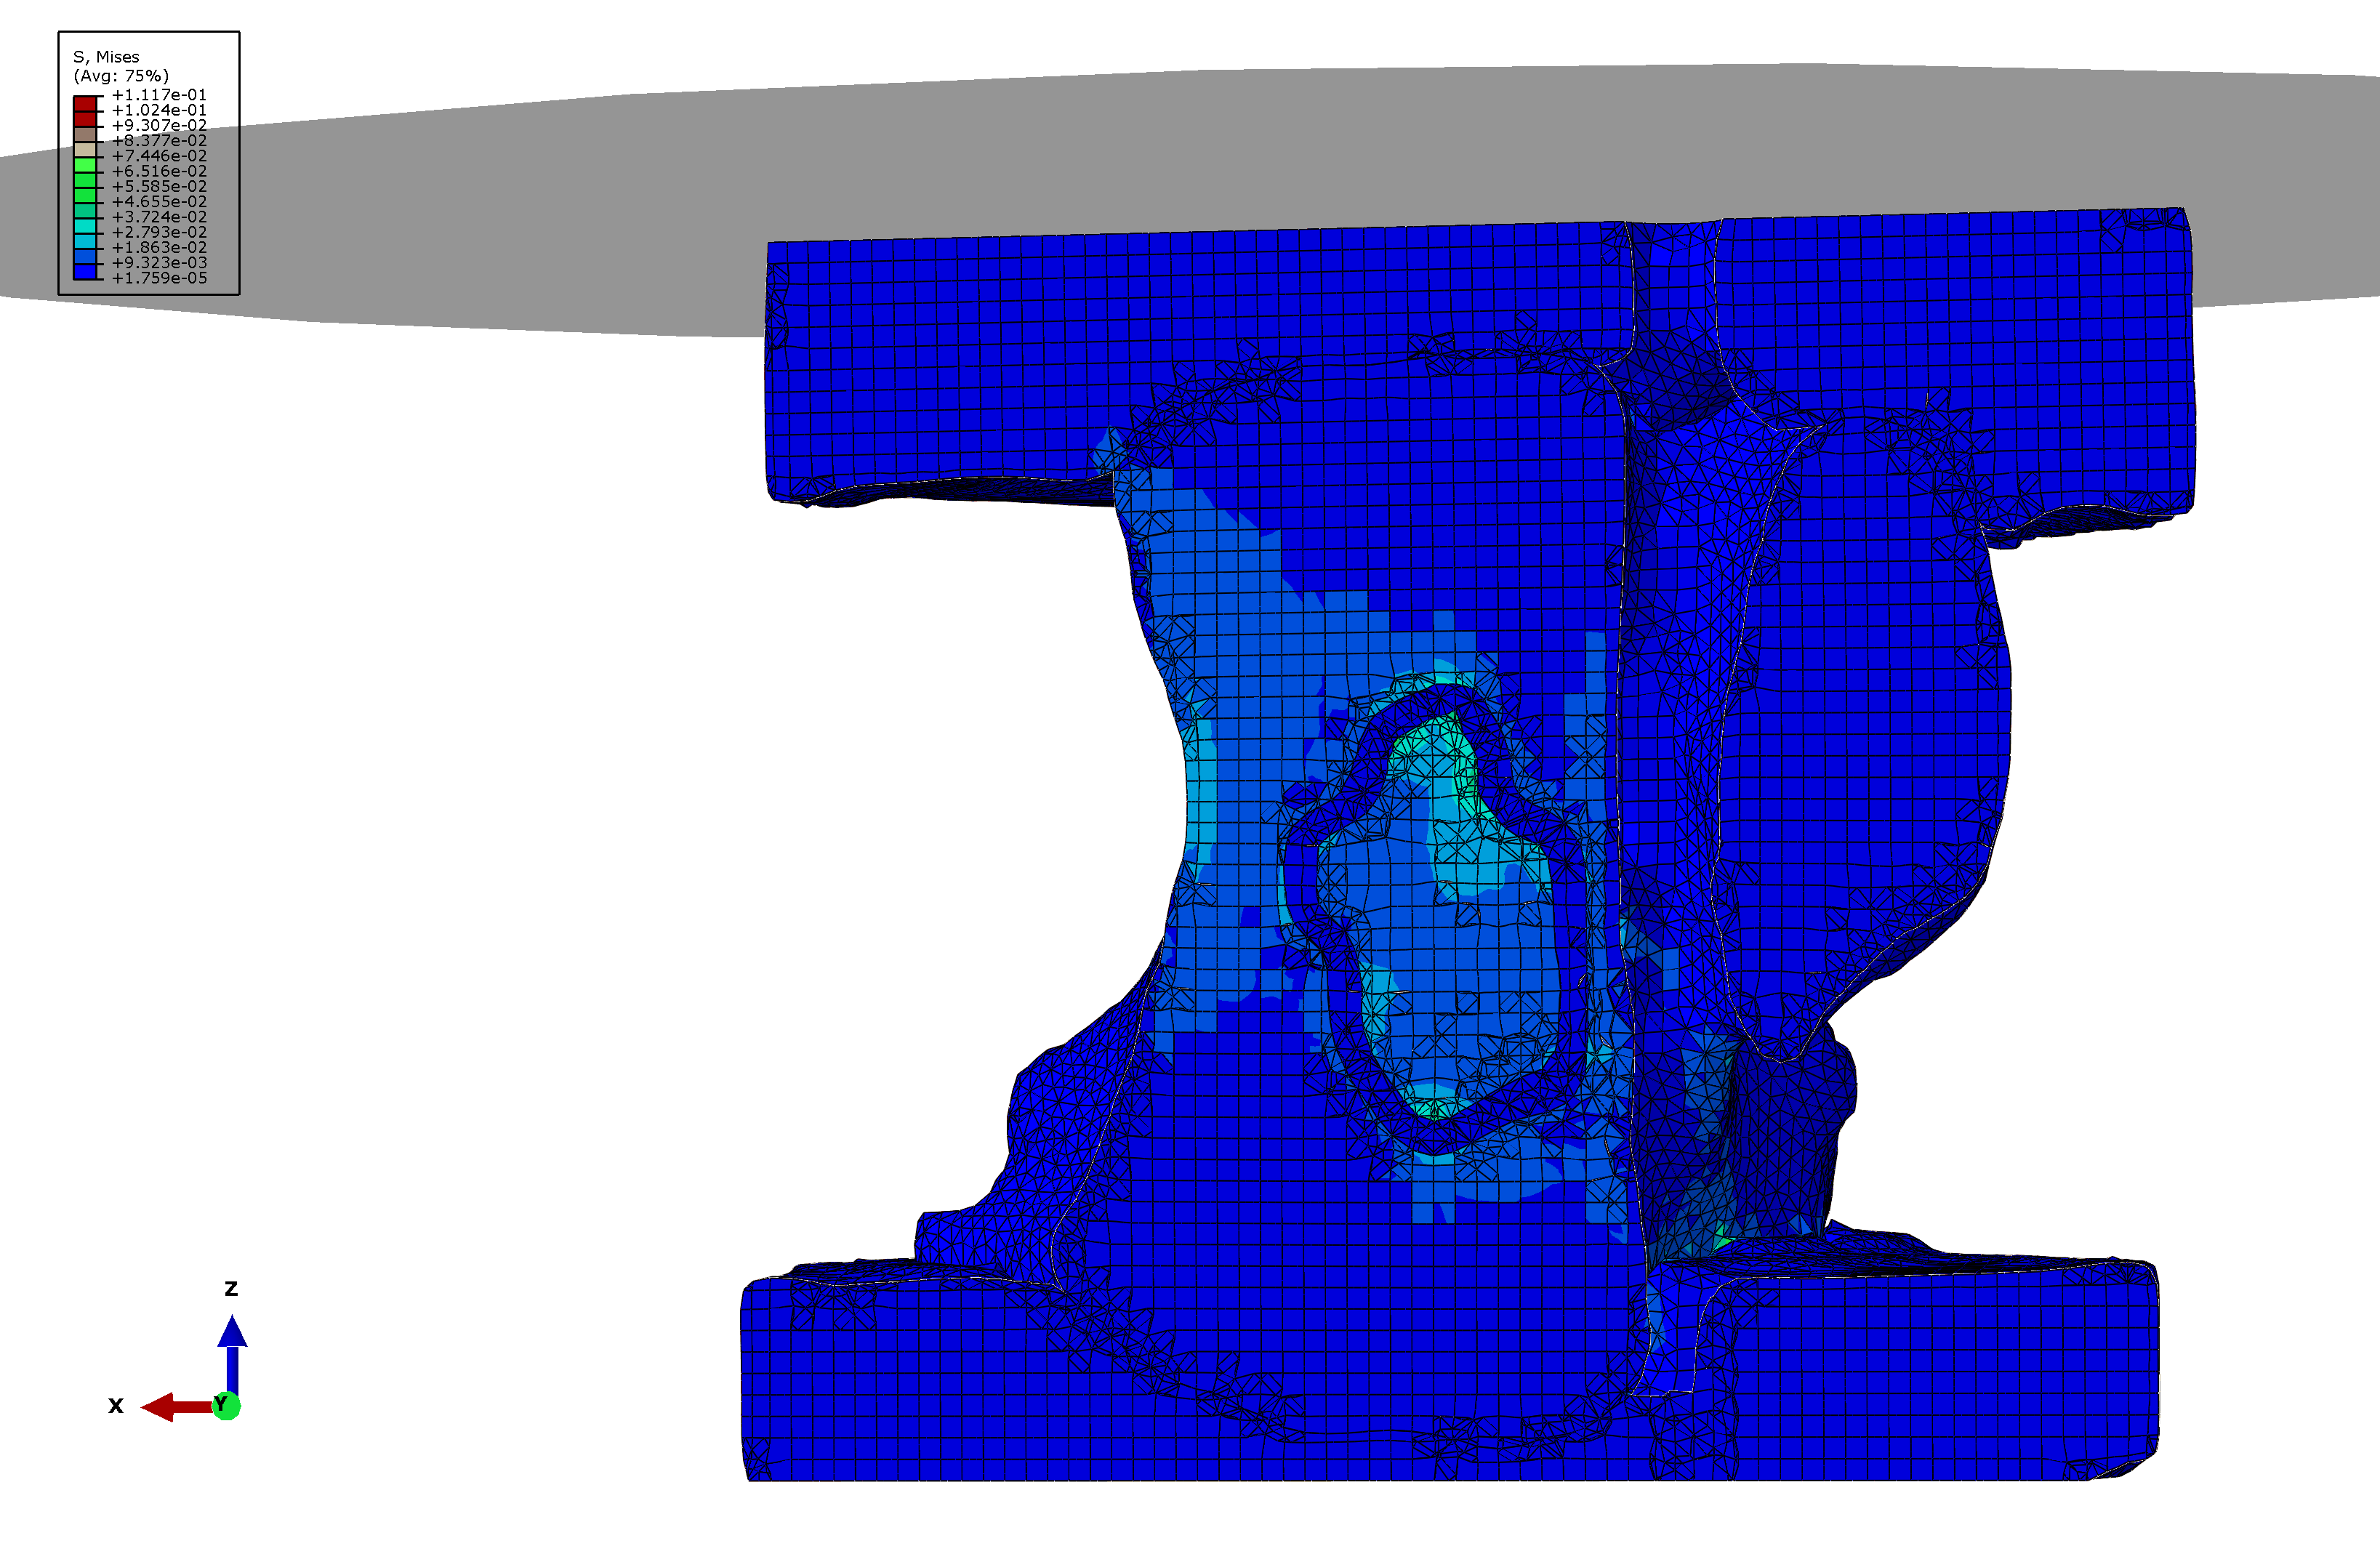
\includegraphics[width=10cm]{images/T9_CC3_postVP_Interface_ABAQUS_All_Side_Stress.png}   & 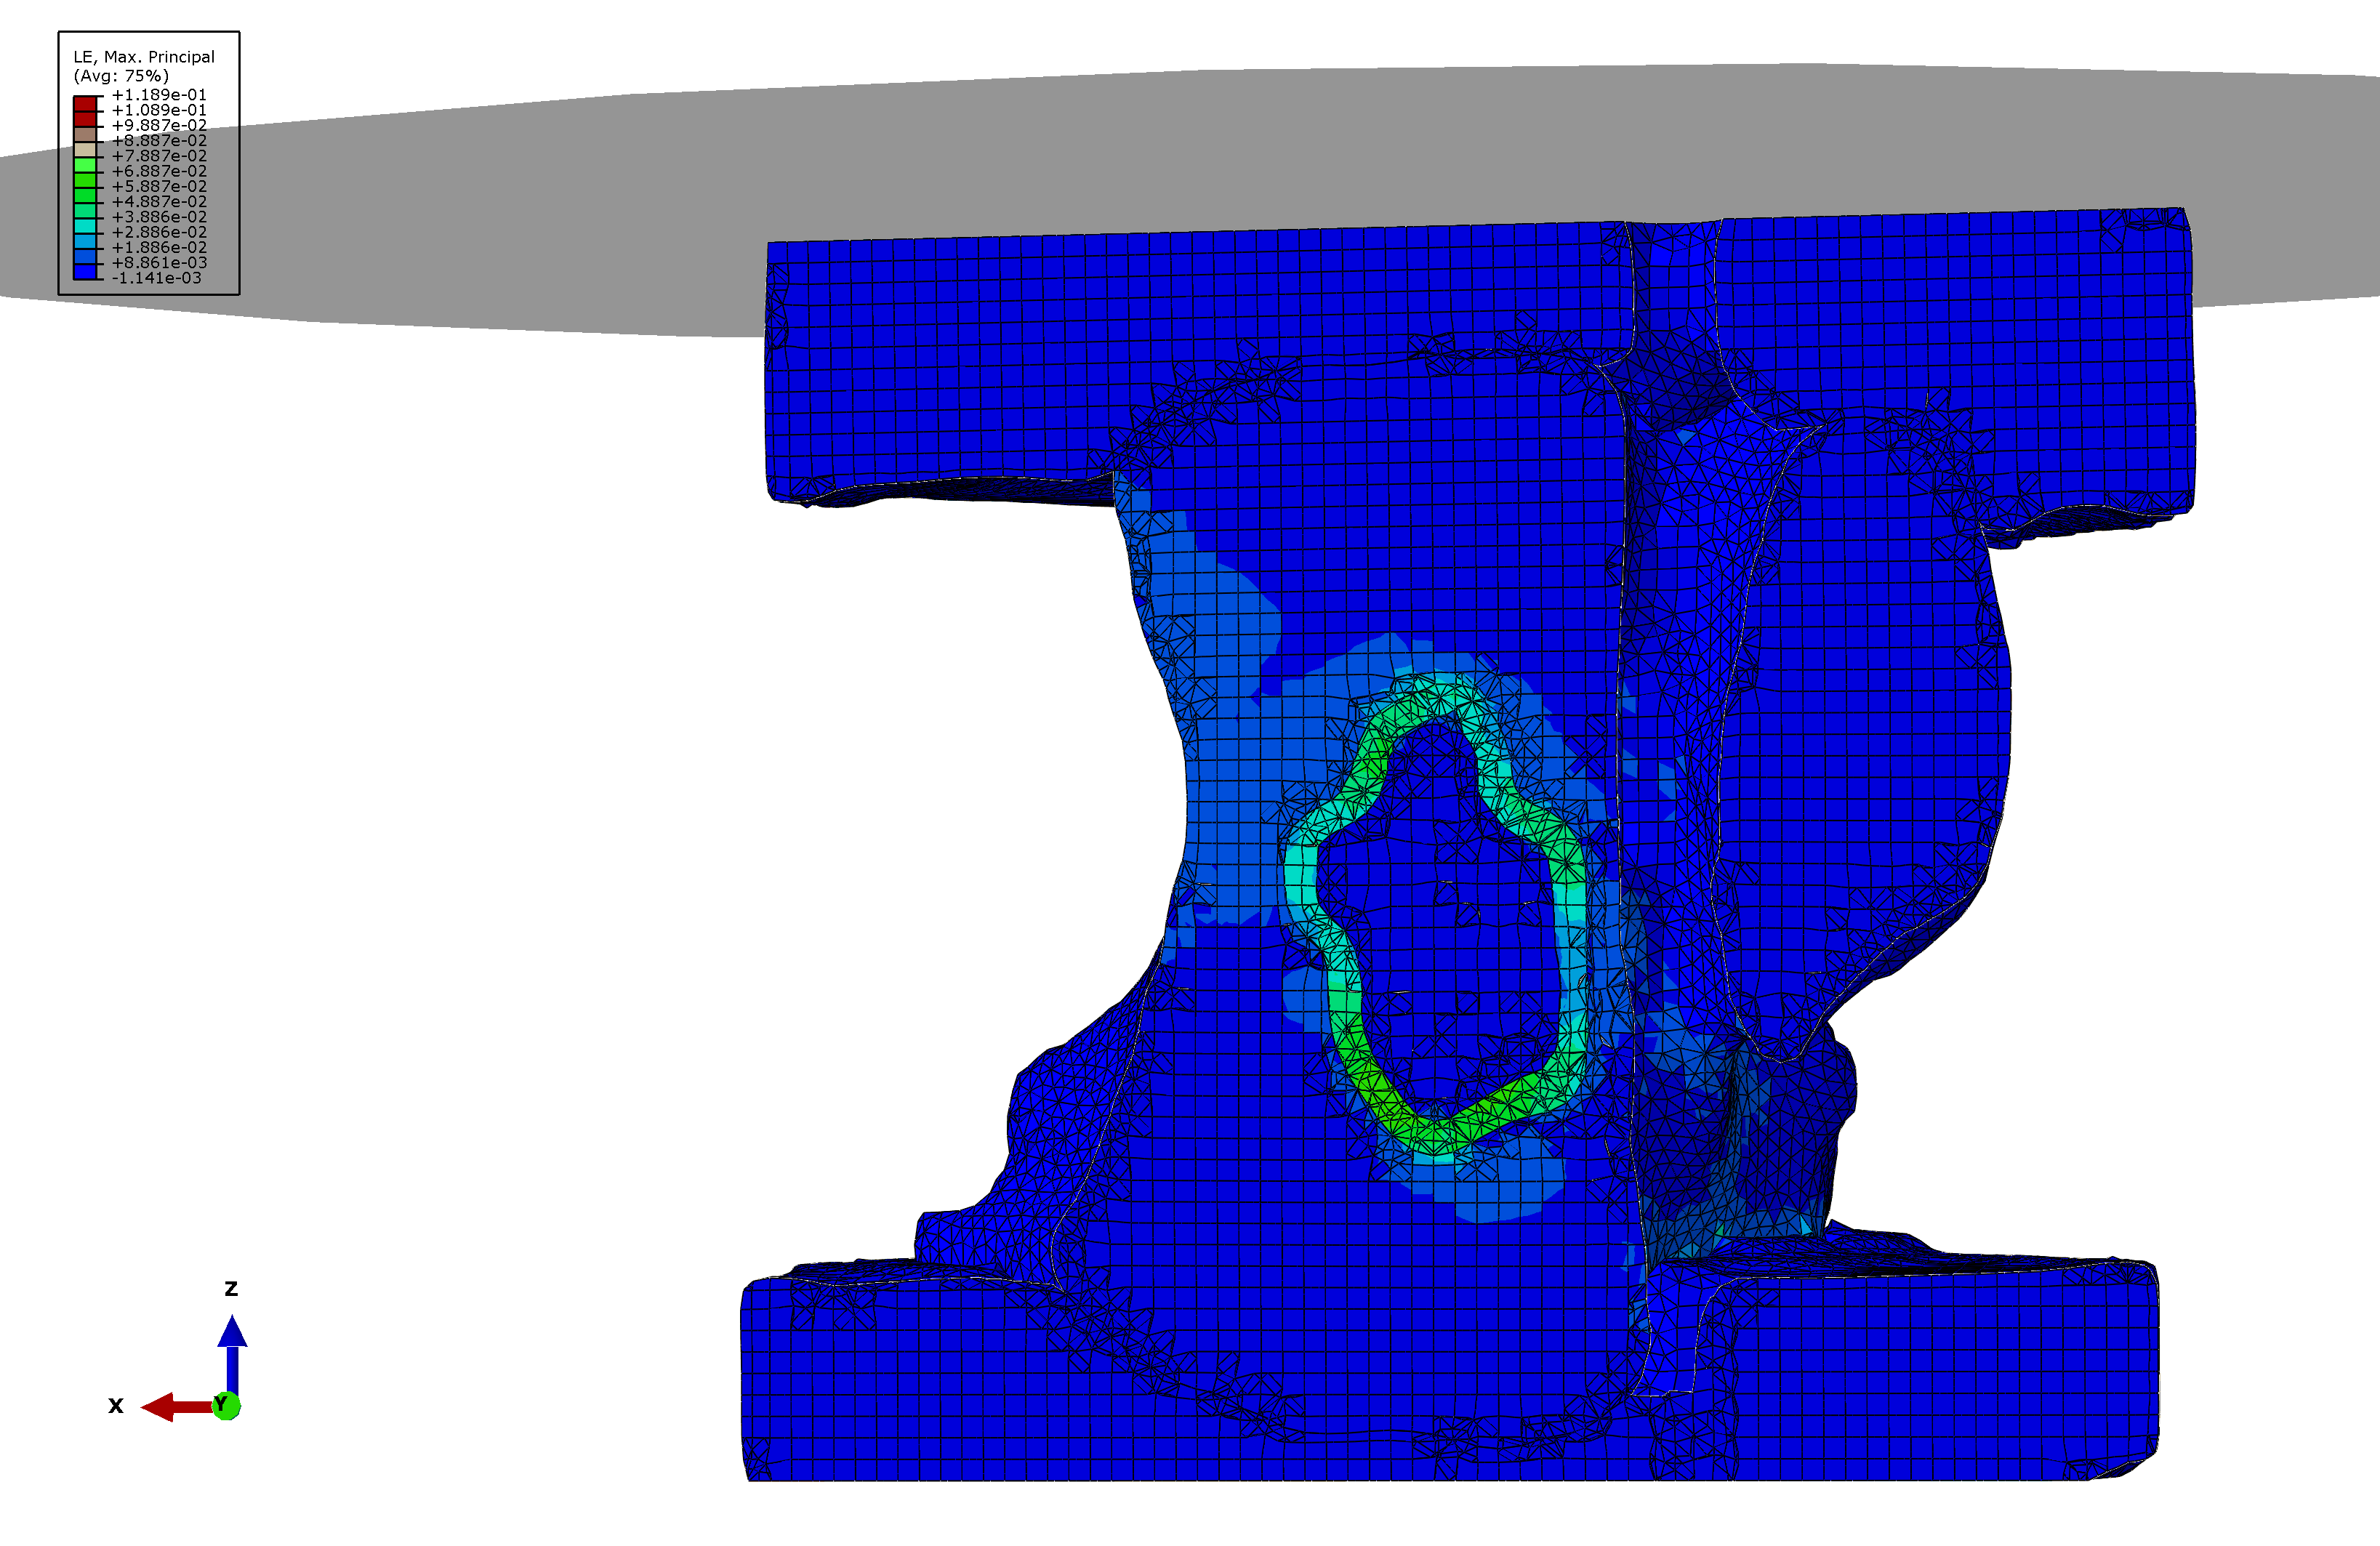
\includegraphics[width=10cm]{images/T9_CC3_postVP_Interface_ABAQUS_All_Side_Strain.png}   & T9 CC3  \begin{itemize} \item Experimental: 	4946.3	N/mm \item Computational:	5186.89 N/mm \item 6.4 \% Fill \end{itemize} \\ \hline 
\end{longtable}


\end{landscape}

\begin{figure}[ht!]
\centering
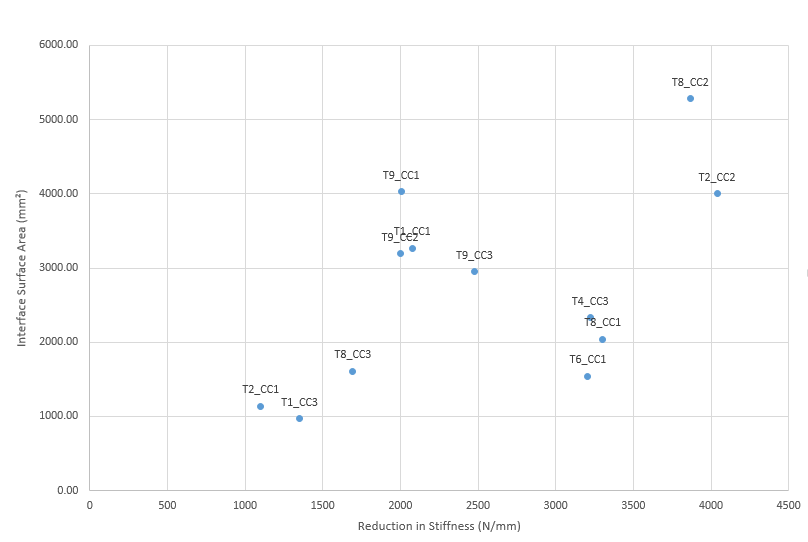
\includegraphics[width=15cm]{images/plot_surf_vs_stiff.png}
\end{figure}

\begin{figure}[ht!]
\centering
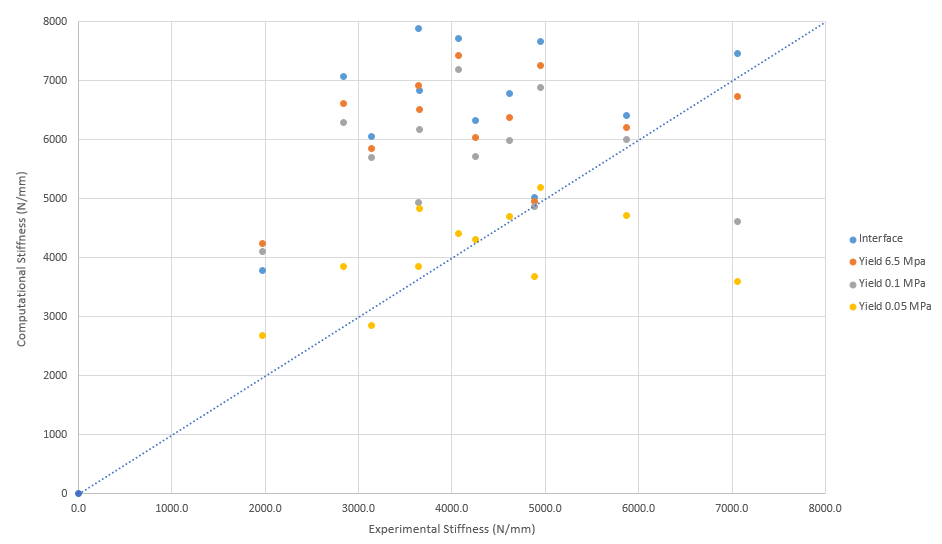
\includegraphics[width=15cm]{images/plot_comp_vs.png}
\end{figure}
\begin{landscape}

\begin{table}[]
\centering
\label{my-label}
\begin{tabular}{l|l|l|l|l|l}
   \hline
Vertebra & Post VP  & Interface                                                  & Yield, 6.5 Mpa                         & Yield, 0.1 MPa                         & Yield, 0.05 MPa                        \\
         &  Experimental                    & Interface: 1.715 GPa & Interface: 1.715 GPa & Interface: 1.715 GPa & Interface: 1.715 GPa\\
         & &  Cement: 1.715 GPa &  Cement: 1.715: GPa &  Cement: 1.715 GPa &  Cement: 1.715 GPa \\ \hline 
T1\_CC1  & 4617.3               & 6779.68                                                    & 6382.72                               & 5996.44                               & 4703.5                                \\
T1\_CC3  & 4883.3               & 5028.41                                                    & 4952.22                               & 4875.58                               & 3677.75                               \\
T2\_CC1  & 1973.8               & 3780.36                                                    & 4244.69                               & 4100.68                               & 2679.83                               \\
T2\_CC2  & 3644.2               & 7892.37                                                    & 6915.46                               & 4931.55                               & 3854.7                                \\
T4\_CC3  & 2838.5               & 7073.76                                                    & 6619.93                               & 6297.05                               & 3851.88                               \\
T6\_CC1  & 3142.1               & 6064.65                                                    & 5858.42                               & 5698.84                               & 2857.61                               \\
T8\_CC1  & 4068.3               & 7722.41                                                    & 7437.22                               & 7194.2                                & 4420.33                               \\
T8\_CC2  & 7057.0               & 7461.93                                                    & 6733.06                               & 4622.13                               & 3596.16                               \\
T8\_CC3  & 5873.1               & 6406.97                                                    & 6206.07                               & 6013.46                               & 4713.04                               \\
T9\_CC1  & 4255.4               & 6323.63                                                    & 6042.86                               & 5717.96                               & 4318.79                               \\
T9\_CC2  & 3654.3               & 6841.63                                                    & 6521.68                               & 6174                                  & 4844.32                               \\
T9\_CC3  & 4946.3               & 7663.55                                                    & 7259.32                               & 6891.98                               & 5186.89                              
\end{tabular}
\end{table}
\end{landscape}
\end{document}
